% Options for packages loaded elsewhere
\PassOptionsToPackage{unicode}{hyperref}
\PassOptionsToPackage{hyphens}{url}
%
\documentclass[
]{article}
\usepackage{amsmath,amssymb}
\usepackage{lmodern}
\usepackage{iftex}
\ifPDFTeX
  \usepackage[T1]{fontenc}
  \usepackage[utf8]{inputenc}
  \usepackage{textcomp} % provide euro and other symbols
\else % if luatex or xetex
  \usepackage{unicode-math}
  \defaultfontfeatures{Scale=MatchLowercase}
  \defaultfontfeatures[\rmfamily]{Ligatures=TeX,Scale=1}
\fi
% Use upquote if available, for straight quotes in verbatim environments
\IfFileExists{upquote.sty}{\usepackage{upquote}}{}
\IfFileExists{microtype.sty}{% use microtype if available
  \usepackage[]{microtype}
  \UseMicrotypeSet[protrusion]{basicmath} % disable protrusion for tt fonts
}{}
\makeatletter
\@ifundefined{KOMAClassName}{% if non-KOMA class
  \IfFileExists{parskip.sty}{%
    \usepackage{parskip}
  }{% else
    \setlength{\parindent}{0pt}
    \setlength{\parskip}{6pt plus 2pt minus 1pt}}
}{% if KOMA class
  \KOMAoptions{parskip=half}}
\makeatother
\usepackage{xcolor}
\usepackage[margin=1in]{geometry}
\usepackage{color}
\usepackage{fancyvrb}
\newcommand{\VerbBar}{|}
\newcommand{\VERB}{\Verb[commandchars=\\\{\}]}
\DefineVerbatimEnvironment{Highlighting}{Verbatim}{commandchars=\\\{\}}
% Add ',fontsize=\small' for more characters per line
\usepackage{framed}
\definecolor{shadecolor}{RGB}{248,248,248}
\newenvironment{Shaded}{\begin{snugshade}}{\end{snugshade}}
\newcommand{\AlertTok}[1]{\textcolor[rgb]{0.94,0.16,0.16}{#1}}
\newcommand{\AnnotationTok}[1]{\textcolor[rgb]{0.56,0.35,0.01}{\textbf{\textit{#1}}}}
\newcommand{\AttributeTok}[1]{\textcolor[rgb]{0.77,0.63,0.00}{#1}}
\newcommand{\BaseNTok}[1]{\textcolor[rgb]{0.00,0.00,0.81}{#1}}
\newcommand{\BuiltInTok}[1]{#1}
\newcommand{\CharTok}[1]{\textcolor[rgb]{0.31,0.60,0.02}{#1}}
\newcommand{\CommentTok}[1]{\textcolor[rgb]{0.56,0.35,0.01}{\textit{#1}}}
\newcommand{\CommentVarTok}[1]{\textcolor[rgb]{0.56,0.35,0.01}{\textbf{\textit{#1}}}}
\newcommand{\ConstantTok}[1]{\textcolor[rgb]{0.00,0.00,0.00}{#1}}
\newcommand{\ControlFlowTok}[1]{\textcolor[rgb]{0.13,0.29,0.53}{\textbf{#1}}}
\newcommand{\DataTypeTok}[1]{\textcolor[rgb]{0.13,0.29,0.53}{#1}}
\newcommand{\DecValTok}[1]{\textcolor[rgb]{0.00,0.00,0.81}{#1}}
\newcommand{\DocumentationTok}[1]{\textcolor[rgb]{0.56,0.35,0.01}{\textbf{\textit{#1}}}}
\newcommand{\ErrorTok}[1]{\textcolor[rgb]{0.64,0.00,0.00}{\textbf{#1}}}
\newcommand{\ExtensionTok}[1]{#1}
\newcommand{\FloatTok}[1]{\textcolor[rgb]{0.00,0.00,0.81}{#1}}
\newcommand{\FunctionTok}[1]{\textcolor[rgb]{0.00,0.00,0.00}{#1}}
\newcommand{\ImportTok}[1]{#1}
\newcommand{\InformationTok}[1]{\textcolor[rgb]{0.56,0.35,0.01}{\textbf{\textit{#1}}}}
\newcommand{\KeywordTok}[1]{\textcolor[rgb]{0.13,0.29,0.53}{\textbf{#1}}}
\newcommand{\NormalTok}[1]{#1}
\newcommand{\OperatorTok}[1]{\textcolor[rgb]{0.81,0.36,0.00}{\textbf{#1}}}
\newcommand{\OtherTok}[1]{\textcolor[rgb]{0.56,0.35,0.01}{#1}}
\newcommand{\PreprocessorTok}[1]{\textcolor[rgb]{0.56,0.35,0.01}{\textit{#1}}}
\newcommand{\RegionMarkerTok}[1]{#1}
\newcommand{\SpecialCharTok}[1]{\textcolor[rgb]{0.00,0.00,0.00}{#1}}
\newcommand{\SpecialStringTok}[1]{\textcolor[rgb]{0.31,0.60,0.02}{#1}}
\newcommand{\StringTok}[1]{\textcolor[rgb]{0.31,0.60,0.02}{#1}}
\newcommand{\VariableTok}[1]{\textcolor[rgb]{0.00,0.00,0.00}{#1}}
\newcommand{\VerbatimStringTok}[1]{\textcolor[rgb]{0.31,0.60,0.02}{#1}}
\newcommand{\WarningTok}[1]{\textcolor[rgb]{0.56,0.35,0.01}{\textbf{\textit{#1}}}}
\usepackage{graphicx}
\makeatletter
\def\maxwidth{\ifdim\Gin@nat@width>\linewidth\linewidth\else\Gin@nat@width\fi}
\def\maxheight{\ifdim\Gin@nat@height>\textheight\textheight\else\Gin@nat@height\fi}
\makeatother
% Scale images if necessary, so that they will not overflow the page
% margins by default, and it is still possible to overwrite the defaults
% using explicit options in \includegraphics[width, height, ...]{}
\setkeys{Gin}{width=\maxwidth,height=\maxheight,keepaspectratio}
% Set default figure placement to htbp
\makeatletter
\def\fps@figure{htbp}
\makeatother
\setlength{\emergencystretch}{3em} % prevent overfull lines
\providecommand{\tightlist}{%
  \setlength{\itemsep}{0pt}\setlength{\parskip}{0pt}}
\setcounter{secnumdepth}{5}
\renewcommand{\and}{\\}
\ifLuaTeX
  \usepackage{selnolig}  % disable illegal ligatures
\fi
\usepackage[]{natbib}
\bibliographystyle{apalike}
\IfFileExists{bookmark.sty}{\usepackage{bookmark}}{\usepackage{hyperref}}
\IfFileExists{xurl.sty}{\usepackage{xurl}}{} % add URL line breaks if available
\urlstyle{same} % disable monospaced font for URLs
\hypersetup{
  pdftitle={Statistical Analysis of High School and College Entrance Exam Scores in Taiwan with Online Data},
  pdfauthor={Christine P. Chai; Microsoft; cpchai21@gmail.com},
  hidelinks,
  pdfcreator={LaTeX via pandoc}}

\title{Statistical Analysis of High School and College Entrance Exam
Scores in Taiwan with Online Data}
\usepackage{etoolbox}
\makeatletter
\providecommand{\subtitle}[1]{% add subtitle to \maketitle
  \apptocmd{\@title}{\par {\large #1 \par}}{}{}
}
\makeatother
\subtitle{A Fully Reproducible Approach with R Markdown}
\author{Christine P.
Chai \and Microsoft \and \href{mailto:cpchai21@gmail.com}{\nolinkurl{cpchai21@gmail.com}}}
\date{\today}

\begin{document}
\maketitle

\renewcommand{\cite}{\citep}

Ongoing work since 2019.

\hypertarget{executive-summary}{%
\section*{Executive Summary}\label{executive-summary}}
\addcontentsline{toc}{section}{Executive Summary}

In this project, we investigate the relationship between high school and
college entrance exam scores in Taiwan using self-reported data online.
The goal is to demonstrate reproducible statistical analysis in
\(\mathsf{R}\) Markdown and LaTeX to PDF. We start by exploring the data
to formulate the problem statement and identify the appropriate model,
which can be an iterative process. We eventually decided on a binary
outcome of the college entrance exams, and hence implemented a logistic
regression to fit the model. We also validated the model with
out-of-sample prediction methods, including cross validation as well as
separate training and testing sets. The end-to-end data analysis can be
compiled with a single button in RStudio, without copying-and-pasting
output from one program to another.

\hypertarget{disclaimer}{%
\section*{Disclaimer}\label{disclaimer}}
\addcontentsline{toc}{section}{Disclaimer}

The opinions and views expressed in this manuscript are those of the
author and do not necessarily state or reflect those of Microsoft. The
author has a statistics and engineering background, without any training
in middle school or high school teaching.

\hypertarget{intro}{%
\section{Introduction}\label{intro}}

The author grew up in Taiwan, so we are curious about the relationship
between the high school entrance exam score percentiles and the college
entrance scores in Taiwan. It seems obvious that a greater percentage of
students from top high schools get admitted to prestigious
universities.\footnote{\url{https://bit.ly/2JSPXKc}} However, the high
school entrance exam is much easier than the college entrance
exam,\footnote{\url{https://www.merit-times.com/NewsPage.aspx?unid=48358}}
so some students studied little in middle school and was able to get
into a good high school. Then some of them kept studying little and
ended up with a bad score on the college entrance exam. On the other
hand, we have also seen some students from non-top-tier high schools
studied very hard, and eventually earned a stellar score in the college
exam.\footnote{\url{https://www.pttweb.cc/bbs/NTU_CK_CM/M.1235046292.A.41C}}
Therefore, we decided to gather data and create our own analysis.

The Taiwan government publishes aggregated data on high school entrance
exam scores\footnote{\url{https://www.ceec.edu.tw/}} and college
entrance exam scores\footnote{\url{https://cap.rcpet.edu.tw/}}
separately, but does not link between the two sets of data by anonymized
individuals. (The closest linkage is the college admission numbers for
selected high schools.\footnote{\url{https://www.ptt.cc/bbs/juniorhigh/M.1407508506.A.1C9.html}})
Therefore, we obtained self-reported data from an existing
post\footnote{\url{https://www.ptt.cc/bbs/SENIORHIGH/M.1432729401.A.995.html}}
in 2015 on PTT, the largest terminal-based bulletin board in Taiwan.
Each of the 197 rows of the data contains an anonymous ID, high school
entrance exam score (in the form of percentile rank), and college
entrance exam score. Since PTT has been advertised to a wide range of
college campuses, many college students as of 2015 were using
PTT.\footnote{PTT Screenshot obtained on June 24, 2022:
  \url{https://imgur.com/Y0pHLiR}} Hence the PTT data could be assumed
to be diverse, i.e., from people with different levels of academic
achievements.

The goal of writing this manuscript is to demonstrate how to perform
data analysis in \texttt{R} using real-life data with a reproducible
workflow. We also make this project open-source on GitHub,\footnote{\url{https://github.com/star1327p/Exam-Scores-PTT}}
so that anyone interested can leverage the data analysis framework as
well as the statistical methodology. The target audience is people with
a basic understanding of statistics, equivalent to taking or having
completed Statistics 101. We start from collecting the data,
preprocessing the data, exploratory analysis, and finally define a
problem statement that can be answered by the data. Then we build the
statistical model, validate the results, and provide our
interpretations. In this way, readers can follow the step-by-step
instructions in this small-scale data science project. Readers will also
learn how to handle issues and continue the analysis in a real
application problem.

The rest of this manuscript is organized as follows. Chapter
\ref{background} gives an overview of the high school and college
entrance exams in Taiwan, and Chapter \ref{data} provides the
description of our dataset. In Chapter \ref{eda}, we start the technical
content with exploratory data analysis, in order to identify and
visualize the distribution of exam scores. Then in Chapter
\ref{linear-reg} we try the linear regression and explain whether this
model is appropriate or not. Chapter \ref{explore-top} further examines
the top scorers, because they typically came from prestigious high
schools and/or colleges. In Chapter \ref{logit-reg}, we modify the
problem statement to binary outcomes and implement the logistic
regression. Then we perform in-sample validation in Chapter
\ref{validation} and out-of-sample validation in Chapter
\ref{out-of-sample}. After the model validation is complete, we provide
a recap of the project in Chapter \ref{recap} and recommend resources
for learning in Chapter \ref{resources}. Finally, we state some personal
remarks in Chapter \ref{personal-remarks}.

\hypertarget{background}{%
\section{Background}\label{background}}

\section*{\textcolor{red}{Unfinished below}}

Elaborate on the following to enhance the background context:

\begin{itemize}
\item
  College entrance exam GSAT and AST: New rules in 2022 (not related to
  COVID)
\item
  COVID-related rules for students who could not attend the exam.\\
  Start writing about 2020, 2021, 2022 for both exams.
\item
  If we continue writing this manuscript in 2023, we absolutely need to
  add the recent changes in 2021 and 2022.
\end{itemize}

\textcolor{red}{This is the file we want to move content into.}

\section*{\textcolor{red}{Unfinished above}}

We briefly explain the high school and college entrance exams in Taiwan
for readers all over the world. Like many other places in Asia, Taiwan
used to put heavy emphasis on standardized tests in high school and
college admissions.\footnote{\url{https://en.wikipedia.org/wiki/Education_in_Taiwan}}
This is different from the US college admission system, which values
more of students' overall qualifications such as extracurricular
activities and personal qualities, not solely on a single standardized
test score.\footnote{\url{https://www.usnews.com/education/best-colleges/articles/college-application-process}}

\textcolor{red}{Continue writing about the Taiwan education system}

Nowadays, Taiwan has added some non-exam components for middle and high
school students, in order to educate them to be well-rounded.\footnote{\url{http://www.ater.org.tw/journal/article/9-6/free/12.pdf}}

Despite multiple attempts of education reform, the high school entrance
exam in Taiwan remains a key part to high school admissions
\citep{chen2017advancing, chen2008strategic}.

What about the college entrance exam in Taiwan? More complicated system.

Changes in the rules every a few years (citation needed).

Although Taiwan's college admission process requires students to submit
their portfolio as part of their application package,\footnote{\url{https://www.reallygood.com.tw/newExam/inside?str=FD956A48971EAE124F46CACDAFD17584}}
students still need to score high enough in the college entrance exam to
pass the initial screening round.\footnote{\url{https://www.thenewslens.com/article/179752}}

\section*{\textcolor{red}{Unfinished above}}

\hypertarget{HighSchool_PR}{%
\subsection{High School Entrance Exam in Taiwan}\label{HighSchool_PR}}

Between 2001 and 2013, the high school entrance exam in Taiwan was
officially called The Basic Competence Test for Junior High School
Students \citep{chou2007schooling}.\footnote{\url{https://bit.ly/2JNQaOI}}
The exam consisted of five subjects (Chinese, English, mathematics,
physical sciences, and social sciences). Note that two exams was held
each year in 2001-2011, and students could take one or both exams
because the difficulty level was about equal.\footnote{\url{https://www.merit-times.com/NewsPage.aspx?unid=120645}}
The first exam was during May-June and the second one was in July. Each
student could use either set of score (typically the better one) to get
their high school placement. The report card contains exam scores for
each subject, the total score, and the percentile rank (PR values from 1
to 99) of the total score. The PR value refers to the percentage of the
student population you scored higher than. For example, PR 86 means you
have a higher score than 86\% of the student population in Taiwan. The
PR values serve as a normalized tool to compare academic achievements
across years.

While the PR values remained consistent, the actual exam score range
varied across years. In 2001-2006, each of the five subjects had a
maximum score of 60, summing up to a total score of 300. In Year 2007,
the independent essay question was added for another 12 points, bringing
up the maximum total score to 312 points.\footnote{\url{https://www.945enet.com.tw/epaper/contents/ha/048/03.htm}}
The scoring of the high school entrance exam had been controversial and
generated much discussion in the news.\footnote{\url{https://web.archive.org/web/20090415123425/http://www.libertytimes.com.tw/2007/new/jun/21/today-life1.htm}}
The main issue was the large score difference between full marks and
getting only one question wrong in a test subject.\footnote{\url{https://blog.xuite.net/wmhsu/twblog/147553826}}
For instance, one could get a 60 with all questions correct in a
subject, but only 55 by missing just one question. The five-point
deduction was regarded as a harsh penalty, given that the knowledge
difference was minimal between a perfect score and a near-perfect
score.\footnote{\url{https://m.xuite.net/blog/chioufatymjh/twblog/130262492}}
Then in Year 2009, the maximum possible score was increased from 312 to
412 points.\footnote{\url{https://blog.cybertranslator.idv.tw/archives/2384}}
Each subject was augmented from 60 to 80 points, and the independent
essay question was still worth 12 points. In the 80-point system,
missing one question would result in a two-point loss from the full
mark, rather than a substantial five or six points.\footnote{\url{https://joan044.pixnet.net/blog/post/255140987}}

In the later stages of this high school entrance exam format, subtle
changes were made in 2011 and 2012, until the final year in 2013. The
high school entrance exam had used the same questions across the whole
country, but in Year 2011, Taipei and its surrounding areas created
their own version of entrance exam.\footnote{\url{https://sites.google.com/site/kleduentrance/01001/07}}
The education officials claimed that more granularity was needed to
distinguish students' academic ability in such competitive
areas.\footnote{\url{https://bit.ly/3Zq2c6e}} Then in Year 2012, the
high school entrance exam was suddenly reduced to one exam per year
instead of two,\footnote{\url{https://m.xuite.net/blog/penghu.dialy/blog/61024095}}
and this continued in Year 2013.\footnote{\url{https://www.ettoday.net/news/20130609/220042.htm}}
In 2012 and 2013, the ``second exam'' was replaced with a pre-exam
admission process: Each middle school could submit formal
recommendations for their students to high schools, with a limited quota
per high school. Students who got admitted by a high school would not
have to take the entrance exam.\footnote{\url{https://news.ltn.com.tw/news/life/breakingnews/537370}}
The controversy was that the changes were implemented quickly, so
neither students nor teachers in middle schools were adequately prepared
to make optimal choices.\footnote{\url{https://www.nhu.edu.tw/~society/e-j/104/a40.htm}}

A major reform came in Year 2014, and the high school entrance exam was
officially replaced with the Comprehensive Assessment Program (CAP) for
Junior High School Students.\footnote{\url{https://bit.ly/41xYSrh}}
Instead of using PR values that emphasized the ranking, CAP provides
each student with seven letter grades for each subject (C, B, B+, B++,
A, A+, A++) and an independent essay score (0-6).\footnote{\url{https://www.parenting.com.tw/article/5049351}}
Each region in Taiwan sets their own rules for high school admission
decisions,\footnote{\url{https://www.facebook.com/JayWangFB/posts/188393636138799/}}
and the CAP score is a necessary but not sufficient condition to get
into a top high school. For example, Taipei and its surrounding areas
award points for completing five semesters of physical education, arts
and humanities, and integrative activities (with an average grade of C
or better).\footnote{\url{https://se.ntpc.edu.tw/12basic/Main/Main1_2}}
Tainan (southern part of Taiwan) also requires additional criteria such
as physical fitness, volunteering activities, and participation in
student organizations.\footnote{\url{https://www.tainan.gov.tw/news_content.aspx?n=13371\&s=3749018}}

\textbf{Remark}: Since the data were self-reported in 2015, the high
school entrance exam scores included only PR values and did not include
any letter grades. In the CAP era starting in 2014, the wide variance of
high school admission requirements makes it more difficult to compare
across students' academic achievements.

\section*{\textcolor{red}{Unfinished below}}

\hypertarget{College_Score}{%
\subsection{College Entrance Exam in Taiwan}\label{College_Score}}

\textcolor{red}{Describe the early admission and the regular admission rules separately.}

\textcolor{red}{Don't go deep into commentaries or how the society reacted to the changes.}

\textcolor{red}{What aggregated data does the Taiwan government publish?}

The college entrance exams in Taiwan are held twice a year; the first
exam is for early admission and the second exam is for regular admission
\citep{chou2015higher}.

The first exam is called the General Scholastic Ability Test (GSAT)
starting in 1994, which is typically held in late January or early
February.\footnote{\url{https://bit.ly/2W0fdUq}} Students can use the
GSAT scores and additional criteria (i.e., their portfolio documents) to
apply to colleges for early admission \citep{hsieh2019preliminary}.

The second exam is called the Advanced Subjects Test (AST) starting in
2002, and it is almost always held on July 1st, 2nd, and 3rd each
year.\footnote{\url{https://bit.ly/2J7YxoW}} In the regular admission
phase, the AST scores are directly used for college placements
\citep{shy2021comparison}, without consideration of the student's
achievements outside the AST scores.\footnote{With limited exceptions of
  GSAT score requirements.
  \url{https://udn.com/news/story/121570/4773243}}

\textcolor{red}{Elaborate on the new regular admission rules starting in 2022}

In 2022, AST was replaced with a completely new scoring
system,\footnote{\url{https://www.ceec.edu.tw/unithome?psid=0J129606443348127072}}
and we do not have sufficient data for this part yet.\footnote{\url{https://www.cw.com.tw/article/5119369}}

\textcolor{red}{Continue writing below}

The GSAT consists of five subjects (Chinese, English, mathematics,
physical sciences, and social sciences), each of which are graded on a 0
to 15 point scale. The GSAT scores are normalized to a range of 0 to 75,
regardless of the difficulty level of GSAT each year. On the other hand,
the scores of AST can vary widely because each subject is scored
separately from 0 to 100. Since the AST scores fluctuate more due to the
difficulty level of the exam questions each year, we decided to use the
GSAT scores as a benchmark of the college exam scores.

The 0 to 15 point scale is calculated in three steps:\footnote{\url{https://bit.ly/3bxIuSn}}

\begin{enumerate}
\def\labelenumi{\arabic{enumi}.}
\tightlist
\item
  Compute the ``top'' as the average raw score of the highest 1\% among
  test takers.
\item
  Divide the number by 15 to get the scale interval.
\item
  Create a table to map raw scores to the 0 to 15 point scale.
\end{enumerate}

For example, if a subject has the ``top'' of 93.45 (max 100), then the
scale interval is 93.45/15 = 6.23, rounded to two decimal points. Zero
point is reserved for absolute zero marks on the exam. A student will
get 1 point for a raw score between 0.01 and 6.23, and 2 points for a
raw score between 6.24 and 12.46, and so on. If we observe from the top
of the scale, a student can get 15 points for a raw score between 87.23
and 100, and 14 points for a raw score between 81.00 and 87.22. Note
that the threshold (87.23) to achieve 15 points is 14 times of the scale
interval (6.23).

\textcolor{red}{Continue writing below}

Starting in 2019, students may choose four of the five subjects for the
GSAT, and the maximum possible score (i.e., full marks) is reduced from
75 to 60.

Starting in 2019, high school students are also required to maintain a
portfolio each semester to document their learning outcomes.\footnote{\url{https://www.108epo.com/courses.php}}

\hypertarget{data}{%
\section{Data Description}\label{data}}

We retrieved data from the SENIORHIGH (high school)\footnote{\url{https://www.ptt.cc/bbs/SENIORHIGH/M.1432729401.A.995.html}}
discussion section on PTT,\footnote{If you have a PTT account, you can
  log into the website using a browser. \url{https://term.ptt.cc/}} the
largest terminal-based bulletin board in Taiwan.\footnote{\url{https://en.wikipedia.org/wiki/PTT_Bulletin_Board_System}}
The data are stored in the file
\texttt{ptt\_SENIORHIGH\_data.csv}.\footnote{\url{https://github.com/star1327p/Exam-Scores-PTT/blob/master/ptt_SENIORHIGH_data.csv}}
The data from PTT are more representative than if we had collected on
our own, because almost anyone could get a PTT account and reply to the
post. The majority of scores were reported in May 2015, and a few scores
were reported in the following month or later. The records indicate that
each respondent had taken the college entrance exam in the year 2015 or
earlier, so we can safely assume that neither of them had taken the new
form of high school entrance exam starting in 2014.

It is a challenge to obtain individual pairs of data as a representative
sample. Although it is easy to send out a spreadsheet and ask our
friends to report their scores anonymously, this approach can result in
a large selection bias. Many of our friends graduated from the same high
school and/or college, so we are likely to have similar entrance exam
scores. That's why we turned to the public forum PTT to reduce selection
bias in the data collection.

Data in the real world are messy, and data scientists spend lots of time
cleaning (preprocessing) the data, i.e., preparing the data for
analysis.\footnote{\url{https://bit.ly/303IWxY}} But data cleaning is a
necessary step for better analysis results, and there are some
visualization examples that demonstrate the importance of preprocessing
the data \citep{chai2020importance}. Our dataset
\texttt{ptt\_SENIORHIGH\_data.csv} is relatively clean, but we still
have to recode and flag some anomaly values.

\hypertarget{flagging-values-in-data}{%
\subsection{Flagging Values in Data}\label{flagging-values-in-data}}

The dataset \texttt{ptt\_SENIORHIGH\_data.csv} contains 197 rows, and
the main variables are:

\begin{itemize}
\tightlist
\item
  \textbf{pttID}: Each person's ID on PTT, which can be anonymous. This
  column serves as the unique identifier of each person.
\item
  \textbf{HighSchool\_PR}: Each person's percentile rank (PR) of the
  high school entrance exam in Taiwan, ranging from 0 to 99.
\item
  \textbf{College\_Score}: Each person's General Scholastic Ability Test
  (GSAT) score, ranging from 0 to 75.
\end{itemize}

There are 6 missing values in \textbf{HighSchool\_PR} and 3 missing
values in \textbf{College\_Score}, so each of them is recorded as ``-1''
(an invalid numerical value for the scores). In the data entry process,
invalid scores like \textbf{HighSchool\_PR} 100 are also treated as
missing.

In some cases, the reported scores can be inaccurate based on the
respondent's description, so we read the comments and manually created
two indicators for this issue. Note that \textbf{inaccurate scores are
still valid}, so we keep them in the data analysis.

\begin{itemize}
\tightlist
\item
  \textbf{HS\_Inacc}: A ``1'' means the reported \textbf{HighSchool\_PR}
  is inaccurate.
\item
  \textbf{CS\_Inacc}: A ``1'' means the reported \textbf{College\_Score}
  is inaccurate.
\end{itemize}

For \textbf{HS\_Inacc} and \textbf{CS\_Inacc}, we set the missing values
to ``0'' because the two flags are binary indicators. Otherwise, the
missing values would show as \texttt{NA}, which are difficult to process
in the code.

\begin{Shaded}
\begin{Highlighting}[]
\NormalTok{data }\OtherTok{=} \FunctionTok{read.csv}\NormalTok{(}\StringTok{"ptt\_SENIORHIGH\_data.csv"}\NormalTok{)}

\FunctionTok{names}\NormalTok{(data)[}\DecValTok{1}\NormalTok{] }\OtherTok{=} \StringTok{"pttID"} \CommentTok{\# system read in as "i..pttID", need to correct this}

\NormalTok{data}\SpecialCharTok{$}\NormalTok{HS\_Inacc[}\FunctionTok{is.na}\NormalTok{(data}\SpecialCharTok{$}\NormalTok{HS\_Inacc)] }\OtherTok{=} \DecValTok{0}
\NormalTok{data}\SpecialCharTok{$}\NormalTok{CS\_Inacc[}\FunctionTok{is.na}\NormalTok{(data}\SpecialCharTok{$}\NormalTok{CS\_Inacc)] }\OtherTok{=} \DecValTok{0}
\end{Highlighting}
\end{Shaded}

One obvious reason of inaccurate scores is that a respondent may comment
that his/her scores are approximate. Moreover, some people reported
their \textbf{HighSchool\_PR} from the mock exam, rather than from the
actual high school entrance exam. In 2012 and 2013, the Ministry of
Education in Taiwan allowed students to apply for high schools with
their grades in middle school. During that time, if a student got
admitted to a high school using this method, he/she would not need to
take the high school entrance exam.\footnote{\url{https://tsjh301.blogspot.com/2014/06/compulsory-education.html}}

For \textbf{College\_Score}, the approximation clause still applies. In
addition, there are two college entrance exams in each school year, and
some students may do much better on the second exam than the first one.
Then they were admitted to a more prestigious school than the first exam
score had indicated, so this is also a form of inaccuracy.

We add two more indicators to signal invalid (impossible) values in
\textbf{HighSchool\_PR} and \textbf{College\_Score}.

\begin{itemize}
\tightlist
\item
  \textbf{HS\_Invalid}: A ``1'' means the reported
  \textbf{HighSchool\_PR} is invalid, i.e., outside the range of 1-99.
\item
  \textbf{CS\_Invalid}: A ``1'' means the reported
  \textbf{College\_Score} is invalid, i.e., outside the range of 1-75.
\end{itemize}

Again, we set \textbf{HS\_Invalid} to ``0'' for a valid
\textbf{HighSchool\_PR}, and set \textbf{CS\_Invalid} to ``0'' for a
valid \textbf{College\_Score}.

\begin{Shaded}
\begin{Highlighting}[]
\NormalTok{data}\SpecialCharTok{$}\NormalTok{HS\_Invalid }\OtherTok{=} \DecValTok{0}
\NormalTok{data}\SpecialCharTok{$}\NormalTok{HS\_Invalid[(data}\SpecialCharTok{$}\NormalTok{HighSchool\_PR }\SpecialCharTok{\textgreater{}} \DecValTok{99}\NormalTok{)}\SpecialCharTok{|}\NormalTok{(data}\SpecialCharTok{$}\NormalTok{HighSchool\_PR }\SpecialCharTok{\textless{}} \DecValTok{1}\NormalTok{)] }\OtherTok{=} \DecValTok{1}

\NormalTok{data}\SpecialCharTok{$}\NormalTok{CS\_Invalid }\OtherTok{=} \DecValTok{0}
\NormalTok{data}\SpecialCharTok{$}\NormalTok{CS\_Invalid[(data}\SpecialCharTok{$}\NormalTok{College\_Score }\SpecialCharTok{\textgreater{}} \DecValTok{75}\NormalTok{)}\SpecialCharTok{|}\NormalTok{(data}\SpecialCharTok{$}\NormalTok{College\_Score }\SpecialCharTok{\textless{}} \DecValTok{1}\NormalTok{)] }\OtherTok{=} \DecValTok{1}
\end{Highlighting}
\end{Shaded}

Finally, we save the clean version to a separate \texttt{.csv} file for
future use.

\begin{Shaded}
\begin{Highlighting}[]
\FunctionTok{write.csv}\NormalTok{(data, }\StringTok{"ptt\_SENIORHIGH\_data\_clean.csv"}\NormalTok{)}
\end{Highlighting}
\end{Shaded}

\hypertarget{data-snapshot}{%
\subsection{Data Snapshot}\label{data-snapshot}}

We show the first 10 rows of data here, and we already see several
anomalies that are flagged. For example, the 1st respondent
\texttt{game275415} provided an approximate value to the
\textbf{HighSchool\_PR}, so we marked this value as inaccurate and a
``1'' in \textbf{HS\_Inacc}. The 4th respondent \texttt{heejung} used
mock exam scores for the \textbf{HighSchool\_PR}, so this score is also
marked as inaccurate. The 6th respondent \texttt{robinyu85} claimed to
not having taken the high school entrance exam at all, so his/her
missing \textbf{HighSchool\_PR} is encoded to ``-1'' and flagged as
invalid.

We also observed that \textbf{pttID} contains some information for
potential inference, although we are not going to use it. For example,
the 6th respondent \texttt{robinyu85} could be someone named Robin Yu,
and the 8th respondent \texttt{godpatrick11} may have the English name
Patrick. Nevertheless, this kind of information is simply a heuristic,
so it is neither sufficient nor appropriate to include in the data
analysis.

\begin{Shaded}
\begin{Highlighting}[]
\NormalTok{data[}\DecValTok{1}\SpecialCharTok{:}\DecValTok{10}\NormalTok{,]}
\end{Highlighting}
\end{Shaded}

\begin{verbatim}
##           pttID HighSchool_PR College_Score HS_Inacc CS_Inacc HS_Invalid CS_Invalid
## 1    game275415            60            50        1        0          0          0
## 2      a2654133            60            52        0        0          0          0
## 3   cookie20125            99            72        0        0          0          0
## 4       heejung            92            54        1        0          0          0
## 5        shun01            87            51        0        0          0          0
## 6     robinyu85            -1            74        0        0          1          0
## 7    allengoose            69            48        0        0          0          0
## 8  godpatrick11            98            60        0        0          0          0
## 9     morgankhs            95            65        0        0          0          0
## 10      jazzard            88            65        0        0          0          0
\end{verbatim}

\hypertarget{bivariate-validation}{%
\subsection{Bivariate Validation}\label{bivariate-validation}}

We need to clean up the data to prepare for the analysis. For example,
we would like to investigate the relationship between
\textbf{HighSchool\_PR} and \textbf{College\_Score}, so we need to
ensure that each record consists of both valid scores. There are 191
records of valid \textbf{HighSchool\_PR} numbers in the data, but if we
consider only the ones with a valid \textbf{College\_Score}, the number
of available records drops to 188. Although which version we use does
not matter much when we look at the univariate distribution, this will
be problematic when we combine the univariate analysis with the
bivariate analysis. Thus, we should use only the 188 records whose
\textbf{College\_Score} numbers are also valid.

\begin{Shaded}
\begin{Highlighting}[]
\CommentTok{\# High school entrance exam scores: Keep only valid numbers}
\NormalTok{uni\_HS\_score }\OtherTok{=}\NormalTok{ data}\SpecialCharTok{$}\NormalTok{HighSchool\_PR[}\FunctionTok{which}\NormalTok{(data}\SpecialCharTok{$}\NormalTok{HS\_Invalid }\SpecialCharTok{==} \DecValTok{0}\NormalTok{)]}
\FunctionTok{length}\NormalTok{(uni\_HS\_score)}
\end{Highlighting}
\end{Shaded}

\begin{verbatim}
## [1] 191
\end{verbatim}

The same requirement also applies to \textbf{College\_Score}. There are
194 records of valid \textbf{College\_Score} numbers in the data, but
only 188 of them also have corresponding valid \textbf{HighSchool\_PR}
numbers.

\begin{Shaded}
\begin{Highlighting}[]
\CommentTok{\# College entrance exam scores: Keep only valid numbers}
\NormalTok{uni\_college\_score }\OtherTok{=}\NormalTok{ data}\SpecialCharTok{$}\NormalTok{College\_Score[}\FunctionTok{which}\NormalTok{(data}\SpecialCharTok{$}\NormalTok{CS\_Invalid }\SpecialCharTok{==} \DecValTok{0}\NormalTok{)]}
\FunctionTok{length}\NormalTok{(uni\_college\_score)}
\end{Highlighting}
\end{Shaded}

\begin{verbatim}
## [1] 194
\end{verbatim}

We do not have enough information to impute the few missing values in
our dataset, so we decided to exclude them from our analysis. There are
nine records with invalid or missing values, and we can locate their
indices in the data.

\begin{Shaded}
\begin{Highlighting}[]
\NormalTok{missing\_rows }\OtherTok{=} \FunctionTok{which}\NormalTok{(data}\SpecialCharTok{$}\NormalTok{HS\_Invalid }\SpecialCharTok{==} \DecValTok{1} \SpecialCharTok{|}\NormalTok{ data}\SpecialCharTok{$}\NormalTok{CS\_Invalid }\SpecialCharTok{==} \DecValTok{1}\NormalTok{)}
\NormalTok{missing\_rows}
\end{Highlighting}
\end{Shaded}

\begin{verbatim}
## [1]   6  19  71  85  88  96 132 183 195
\end{verbatim}

\textbf{Remark}: With larger and/or more complex datasets, researchers
often apply record linkage methods \citep{dusetzina2014overview} to
impute missing or erroneous values in one dataset from another. This is
outside the scope of this manuscript.

Now we build the \texttt{R} dataframe \texttt{data\_corr} (short for
``data correlation'') for the bivariate analysis. This dataframe
excludes any record with at least one missing value in
\textbf{HighSchool\_PR} or \textbf{College\_Score}.

\begin{Shaded}
\begin{Highlighting}[]
\CommentTok{\# Remove missing data}
\NormalTok{data\_corr }\OtherTok{=}\NormalTok{ data[}\SpecialCharTok{{-}}\NormalTok{missing\_rows,]}
\end{Highlighting}
\end{Shaded}

Again, we show the first 10 rows of \texttt{data\_corr}, and all values
in \texttt{HighSchool\_PR} and \texttt{College\_Score} are valid. The
indicators \texttt{HS\_Invalid} and \texttt{CS\_Invalid} should be zero
throughout this version of data.

\begin{Shaded}
\begin{Highlighting}[]
\NormalTok{data\_corr[}\DecValTok{1}\SpecialCharTok{:}\DecValTok{10}\NormalTok{,]}
\end{Highlighting}
\end{Shaded}

\begin{verbatim}
##           pttID HighSchool_PR College_Score HS_Inacc CS_Inacc HS_Invalid CS_Invalid
## 1    game275415            60            50        1        0          0          0
## 2      a2654133            60            52        0        0          0          0
## 3   cookie20125            99            72        0        0          0          0
## 4       heejung            92            54        1        0          0          0
## 5        shun01            87            51        0        0          0          0
## 7    allengoose            69            48        0        0          0          0
## 8  godpatrick11            98            60        0        0          0          0
## 9     morgankhs            95            65        0        0          0          0
## 10      jazzard            88            65        0        0          0          0
## 11     ksacball            99            70        0        0          0          0
\end{verbatim}

The function \texttt{dim} retrieves the dimensions of the \texttt{R}
dataframe \texttt{data\_corr}. The output reveals that the dataset
contains 188 rows and 7 columns, where the 188 rows refer to the 188
records with a valid score in both \texttt{HighSchool\_PR} and
\texttt{College\_Score}.

\begin{Shaded}
\begin{Highlighting}[]
\FunctionTok{dim}\NormalTok{(data\_corr)}
\end{Highlighting}
\end{Shaded}

\begin{verbatim}
## [1] 188   7
\end{verbatim}

Alternatively, we can also use the function \texttt{length} to find the
number of elements in an array. This shows both columns
\texttt{HighSchool\_PR} and \texttt{College\_Score} contain 188 elements
each. Note that \texttt{length} does not distinguish between missing and
non-missing values. A missing element, often denoted as \texttt{NA}, is
still counted as one element.

\begin{Shaded}
\begin{Highlighting}[]
\FunctionTok{length}\NormalTok{(data\_corr}\SpecialCharTok{$}\NormalTok{HighSchool\_PR)}
\end{Highlighting}
\end{Shaded}

\begin{verbatim}
## [1] 188
\end{verbatim}

\begin{Shaded}
\begin{Highlighting}[]
\FunctionTok{length}\NormalTok{(data\_corr}\SpecialCharTok{$}\NormalTok{College\_Score)}
\end{Highlighting}
\end{Shaded}

\begin{verbatim}
## [1] 188
\end{verbatim}

\textbf{Remark}: Readers new to \texttt{R} programming may wonder where
we can find the type of each object, in order to determine how to
proceed next. The function \texttt{class} returns the type of the input
object, and the output confirms that \texttt{data\_corr} is an
\texttt{R} dataframe. Then we can leverage the functions available for
this data structure.

\begin{Shaded}
\begin{Highlighting}[]
\FunctionTok{class}\NormalTok{(data\_corr)}
\end{Highlighting}
\end{Shaded}

\begin{verbatim}
## [1] "data.frame"
\end{verbatim}

\hypertarget{eda}{%
\section{Exploratory Data Analysis}\label{eda}}

Before we perform any statistical modeling, we need to observe the data
and this step is called exploratory data analysis. The exploratory phase
allows us to identify patterns, detect anomalies, and verify assumptions
in the data.\footnote{\url{https://blog.eduonix.com/bigdata-and-hadoop/importance-exploratory-data-analysis-ml-modelling}}
This is an important but often overlooked step in data analysis, and
failure to explore the data can lead to inefficiencies such as accurate
models on the wrong data.\footnote{\url{https://towardsdatascience.com/exploratory-data-analysis-topic-that-is-neglected-in-data-science-projects-9962ae078a56}}

Therefore, we start with examining the trends of the two main variables,
\textbf{HighSchool\_PR} and \textbf{College\_Score}. For each variable,
we observe the values and summarize them in a histogram as part of the
univariate analysis. Then we investigate the relationship between the
two variables, i.e., bivariate exploration.

\hypertarget{high-school-entrance-exam-scores-percentile-rank}{%
\subsection{High School Entrance Exam Scores (Percentile
Rank)}\label{high-school-entrance-exam-scores-percentile-rank}}

We show the descriptive statistics of \textbf{HighSchool\_PR} in our
data, i.e., the percentile rank of high school entrance exam scores. The
invalid or missing values are removed beforehand. The \texttt{summary}
function returns the minimum, 1st quartile, median, mean, 3rd quartile,
and maximum from the input data.

\begin{itemize}
\tightlist
\item
  \textbf{Minimum}: The smallest value in the data.
\item
  \textbf{1st Quartile}: The value where 25\% of the data is below this
  point; that is, the middle value between the minimum and the median.
\item
  \textbf{Median}: The value where 50\% of the data is below this point,
  and 50\% of the data is above this point.
\item
  \textbf{Mean}: The arithmetic mean, which is calculated as the sum of
  the data divided by the number of the points.
\item
  \textbf{3rd Quartile}: The value where 75\% of the data is below this
  point; that is, the middle value between the median and the maximum.
\item
  \textbf{Maximum}: The largest value in the data.
\end{itemize}

\begin{Shaded}
\begin{Highlighting}[]
\FunctionTok{summary}\NormalTok{(uni\_HS\_score)}
\end{Highlighting}
\end{Shaded}

\begin{verbatim}
##    Min. 1st Qu.  Median    Mean 3rd Qu.    Max. 
##   51.00   85.00   92.00   89.82   97.00   99.00
\end{verbatim}

\textbf{Remark}: Note that we used the full univariate set of
\textbf{HighSchool\_PR} available, rather than taking only those with a
valid \textbf{College\_Score}. The reason is that we wanted to keep as
many records as possible. We can do a quick sensitivity analysis here,
and the summary statistics are very similar after we exclude the few
records without a valid \textbf{College\_Score}.

\begin{Shaded}
\begin{Highlighting}[]
\FunctionTok{summary}\NormalTok{(data\_corr}\SpecialCharTok{$}\NormalTok{HighSchool\_PR)}
\end{Highlighting}
\end{Shaded}

\begin{verbatim}
##    Min. 1st Qu.  Median    Mean 3rd Qu.    Max. 
##    51.0    85.0    92.0    89.7    97.0    99.0
\end{verbatim}

In the univariate analysis, the 1st quartile of \textbf{HighSchool\_PR}
is 85, which means only 25\% of the respondents have a percentile rank
(PR) below 85. Hence 75\% of the respondents have a percentile rank (PR)
at least 85, i.e., in the top 15\% of the high school entrance exam. The
median (92) is higher than the mean (89-90), indicating that the
distribution is left-skewed. Half of the respondents scored
\textbf{HighSchool\_PR} 92 or better, and we have few samples of the
lower end of the high school entrance exam. In fact, the lowest score we
obtained in the data is already 51 -- still slightly above the national
median score (50). The maximum is capped at 99.

The histogram shows a left-skewed distribution, and we can see a long
tail to the left. Since our data are self-reported by respondents, the
ones with higher scores are more likely to report, resulting in survey
non-response bias. It is also possible that many students with extremely
low \textbf{HighSchool\_PR} chose not to attend college, so they would
not have a \textbf{College\_Score} to respond to the survey.

\begin{Shaded}
\begin{Highlighting}[]
\FunctionTok{hist}\NormalTok{(uni\_HS\_score, }\AttributeTok{main =} \StringTok{"Histogram of HighSchool\_PR"}\NormalTok{, }\AttributeTok{xlab=}\StringTok{"HighSchool\_PR"}\NormalTok{)}
\end{Highlighting}
\end{Shaded}

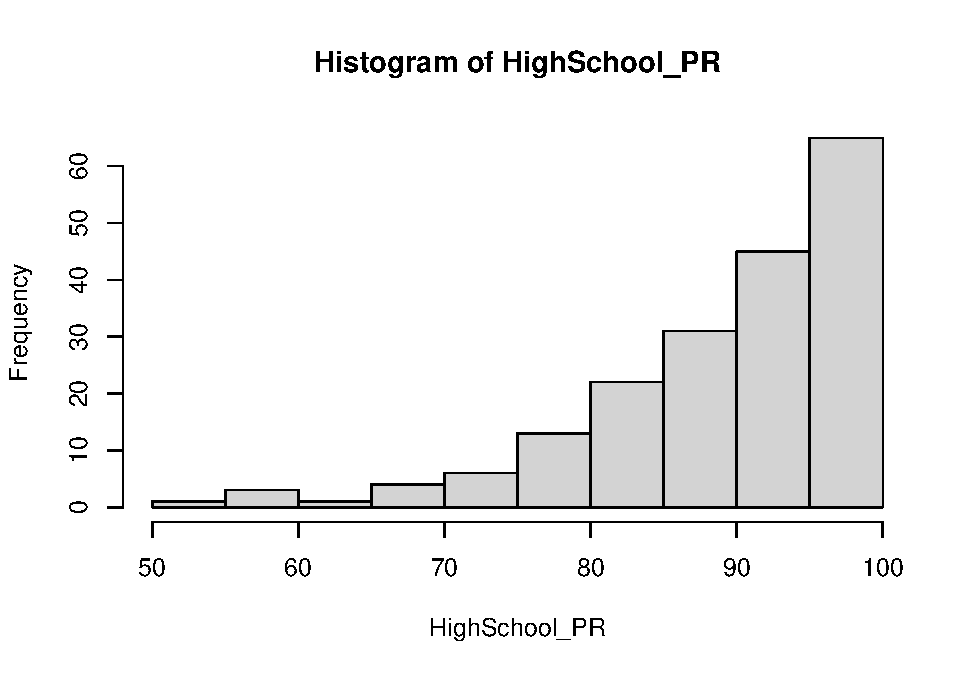
\includegraphics{PTT_Analysis_of_Test_Scores_Unfinished_files/figure-latex/high-school-pr-histogram-1.pdf}

If we were to take a sufficiently large random sample from the full
database of \textbf{HighSchool\_PR} in Taiwan, the minimum should be 1
and the maximum would still be at 99. However, the
\textbf{HighSchool\_PR} is the national percentile rank itself, so the
1st quartile should be around 25, median and mean both around 50, and
the 3rd quartile around 75.

As a baseline, we also simulate this random sample by generating data
from a \textbf{discrete} uniform distribution between 1 and 99. We
manually take a random sample of the same size as the univariate
\textbf{HighSchool\_PR} from the integers 1, 2, \ldots, 99, and we
sample with replacement to allow duplicate values. Note that the
function
\texttt{runif}\footnote{The function name \texttt{runif} is pronounced as \texttt{r-unif}, not \texttt{run-if}.}
in the \texttt{stats} package generates samples from the
\textbf{continuous} uniform distribution, and that's why we did not use
\texttt{runif} here.

\begin{Shaded}
\begin{Highlighting}[]
\NormalTok{possible\_values }\OtherTok{=} \FunctionTok{c}\NormalTok{(}\DecValTok{1}\SpecialCharTok{:}\DecValTok{99}\NormalTok{)}

\FunctionTok{set.seed}\NormalTok{(}\DecValTok{67}\NormalTok{)}
\CommentTok{\# sample with replacement}
\NormalTok{random\_sample }\OtherTok{=} \FunctionTok{sample}\NormalTok{(possible\_values, }\AttributeTok{size=}\FunctionTok{length}\NormalTok{(uni\_HS\_score), }\AttributeTok{replace=}\ConstantTok{TRUE}\NormalTok{)}
\FunctionTok{print}\NormalTok{(random\_sample)}
\end{Highlighting}
\end{Shaded}

\begin{verbatim}
##   [1] 43 84 97 78 71 33 94 45 52 45 32  1 68 80 24  5 96 27 62  3 24 48 63 85 52
##  [26] 99 79 30 73 63 59 19 10 70 67 77 76 59 80 11  4 43 12 33 22 45 12 68 23 98
##  [51] 13  1 96 28 53 74 19 11 42 77 75 31 94 15 31 75 76 63 37 77 52 86 64 15 32
##  [76] 97  4 18 11 16 36 70 18 91 23 39 70 58 71 90  4 32 91 19 83 16 67 88 71 16
## [101] 10  7 65 42 56 19 79  7 26 74  4 32 83 98 77 61 49 66 46  6 17 48 84 41 65
## [126] 64 38 45 79 18 55 23 37 69  9 63 41 73 35 55  2 38 23 58 16 91 94 94 16 62
## [151]  3 57 49 36 84 94 45 62 53 29 81 73 87 22 99 36 29 82  6 84  7 65 18 33 68
## [176] 35 84 67  3 57 24 13 77 14 49 25 83 41  8 68  6
\end{verbatim}

As we can see, the simulated random sample has median and mean close to
50. The 1st quartile is near 25, and the 3rd quartile is near 75. The
simulated sample is to demonstrate a nationally representative sample of
\textbf{HighSchool\_PR}. Nevertheless, this would not be appropriate for
the evaluation of the relationship between \textbf{HighSchool\_PR} and
\textbf{College\_Score}, because students with extremely low
\textbf{HighSchool\_PR} may decide not to attend college at all.

\begin{Shaded}
\begin{Highlighting}[]
\FunctionTok{summary}\NormalTok{(random\_sample)}
\end{Highlighting}
\end{Shaded}

\begin{verbatim}
##    Min. 1st Qu.  Median    Mean 3rd Qu.    Max. 
##    1.00   23.00   49.00   48.67   73.50   99.00
\end{verbatim}

The histogram of the simulated random sample is flat, as what we expect
from a discrete uniform distribution.

\begin{Shaded}
\begin{Highlighting}[]
\FunctionTok{hist}\NormalTok{(random\_sample, }\AttributeTok{main =} \StringTok{"Histogram of Simulated Random Sample"}\NormalTok{, }\AttributeTok{xlab=}\StringTok{"HighSchool\_PR"}\NormalTok{)}
\end{Highlighting}
\end{Shaded}

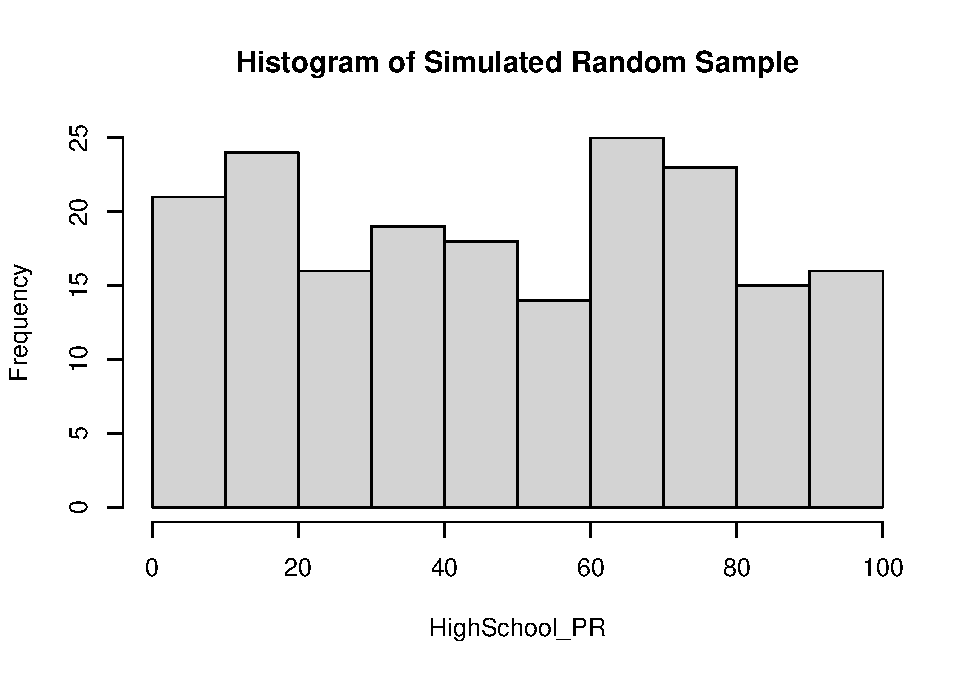
\includegraphics{PTT_Analysis_of_Test_Scores_Unfinished_files/figure-latex/random-data-histogram-1.pdf}

\hypertarget{college-entrance-exam-scores}{%
\subsection{College Entrance Exam
Scores}\label{college-entrance-exam-scores}}

Similarly, we also show the descriptive statistics of
\textbf{College\_Score}, i.e., the college entrance exam scores between
1 and 75. The distribution is also left-skewed, but less extreme than
\textbf{HighSchool\_PR}. The median of \textbf{College\_Score} is 64.5,
indicating that 50\% of the respondents have \textbf{College\_Score} 65
or higher. The 3rd quartile is already at 69, so the top score range
69-75 accounts for 25\% of the respondents. This is much higher than the
national average.

\begin{Shaded}
\begin{Highlighting}[]
\FunctionTok{summary}\NormalTok{(uni\_college\_score)}
\end{Highlighting}
\end{Shaded}

\begin{verbatim}
##    Min. 1st Qu.  Median    Mean 3rd Qu.    Max. 
##    34.0    58.0    64.5    62.7    69.0    75.0
\end{verbatim}

As a sensitivity analysis check, we also examine the \texttt{summary} of
the \textbf{College\_Score} datapoints only when they have a
corresponding valid \textbf{HighSchool\_PR}. The distribution is almost
the same.

\begin{Shaded}
\begin{Highlighting}[]
\FunctionTok{summary}\NormalTok{(data\_corr}\SpecialCharTok{$}\NormalTok{College\_Score)}
\end{Highlighting}
\end{Shaded}

\begin{verbatim}
##    Min. 1st Qu.  Median    Mean 3rd Qu.    Max. 
##   34.00   58.00   64.00   62.49   69.00   75.00
\end{verbatim}

According to the reference score table\footnote{\url{https://bit.ly/3bAYOvO}}
from Wikipedia, the 88th percentile of the college entrance score
fluctuates around 60 in Years 2004-2010, and 62-65 in Years 2011-2018.
Since the median of \textbf{College\_Score} is 64.5, we can infer that
at least 50\% of the respondents scored in the top 12\% of the college
entrance exam. On the other hand, the reference score table also shows
that the 75th percentile of the college entrance score is between 53 and
58 in Years 2004-2018. The PTT data's 1st quantile is already at 58, so
we can also infer that at least 75\% of the respondents scored in the
top 25\% of the college entrance exam.

Since PTT contains forums for several prestigious universities in
Taiwan, it is no surprise that many users attended these colleges
because they scored well on the college entrance exam. Nevertheless, PTT
does not limit registration to students of these colleges, so the
population of PTT is relatively diverse but still not very
representative of the whole student population.

The histogram for \textbf{College\_Score} also shows a left-skewed
distribution, but not as extreme as \textbf{HighSchool\_PR}. Note that
right-skewed distributions are more common in real life, such as
employee salaries and movie ticket sales.\footnote{\url{https://www.statology.org/positively-skewed-distribution-examples/}}

\begin{Shaded}
\begin{Highlighting}[]
\FunctionTok{hist}\NormalTok{(uni\_college\_score, }\AttributeTok{main=}\StringTok{"Histogram of College\_Score"}\NormalTok{,}
     \AttributeTok{xlab=}\StringTok{"College\_Score (max possible is 75)"}\NormalTok{,}\AttributeTok{xlim=}\FunctionTok{c}\NormalTok{(}\DecValTok{30}\NormalTok{,}\DecValTok{80}\NormalTok{))}
\end{Highlighting}
\end{Shaded}

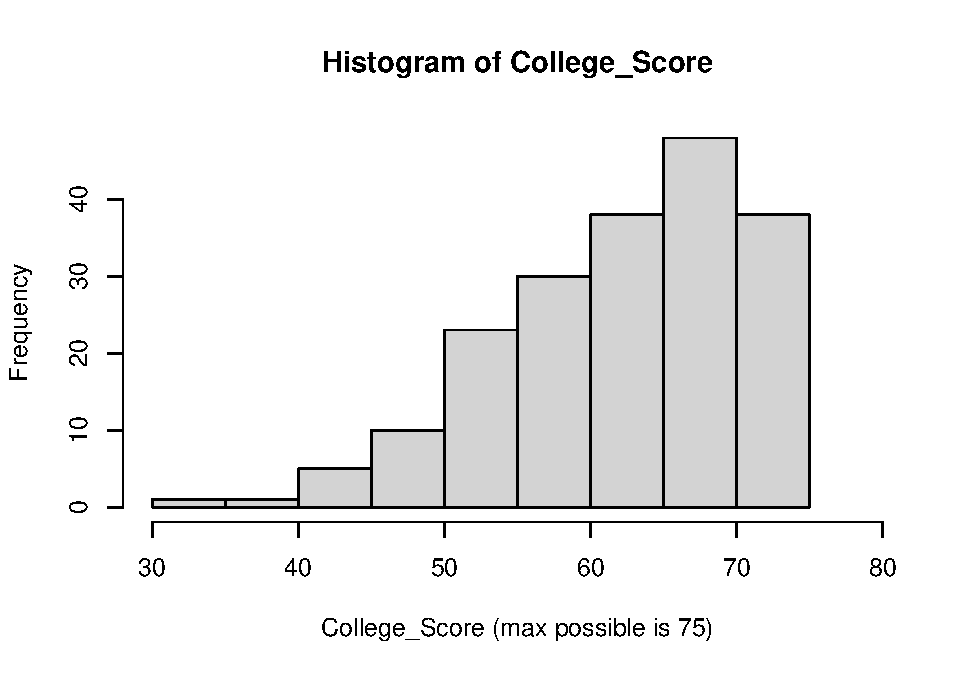
\includegraphics{PTT_Analysis_of_Test_Scores_Unfinished_files/figure-latex/college-score-histogram-1.pdf}

Unlike the case of \textbf{HighSchool\_PR}, we do not think it is
appropriate to simulate a random sample for \textbf{College\_Score}
across years in general. First, \textbf{College\_Score} are not
percentile ranks like \textbf{HighSchool\_PR}, and there is no
statistical nature of how the \textbf{College\_Score} distribution
should look like. Moreover, the exact distribution of
\textbf{College\_Score} differs greatly due to the varying difficulty
levels each year. For example, the 88th percentile of
\textbf{College\_Score} was 65 in 2014 and 59 in 2007.\footnote{\url{https://bit.ly/2W0fdUq}}
The 6-point difference in the score is large enough for an applicant to
get admitted to a lower or higher tier of universities.

In Section \ref{College_Score}, we mentioned that the Taiwan government
published detailed statistics of the \textbf{College\_Score} each year,
including the five indicators (88th, 75th, 50th, 25th, 12th percentile)
of each subject and the total score. However, since our data sample
contains \textbf{College\_Score} across several years, it is not
meaningful to generate a simulated distribution here.

\hypertarget{bivariate}{%
\subsection{Bivariate Exploration}\label{bivariate}}

Next, we create a bivariate scatterplot of \textbf{HighSchool\_PR} and
\textbf{College\_Score} to examine the relationship between the two
scores. Obviously, a respondent needs a valid score in both to be
included in the bivariate scatterplot. Just like what we observed in the
univariate plots, both variables are largely concentrated towards the
maximum possible scores. The bivariate scatterplot shows a funnel shape
-- respondents with lower \textbf{HighSchool\_PR} have higher variance
in \textbf{College\_Score}.

\begin{Shaded}
\begin{Highlighting}[]
\FunctionTok{plot}\NormalTok{(data\_corr}\SpecialCharTok{$}\NormalTok{HighSchool\_PR, data\_corr}\SpecialCharTok{$}\NormalTok{College\_Score,}
     \AttributeTok{main =} \StringTok{"High School and College Entrance Exam Scores"}\NormalTok{,}
     \AttributeTok{xlab=}\StringTok{"HighSchool\_PR"}\NormalTok{,}
     \AttributeTok{ylab=}\StringTok{"College\_Score"}\NormalTok{)}
\end{Highlighting}
\end{Shaded}

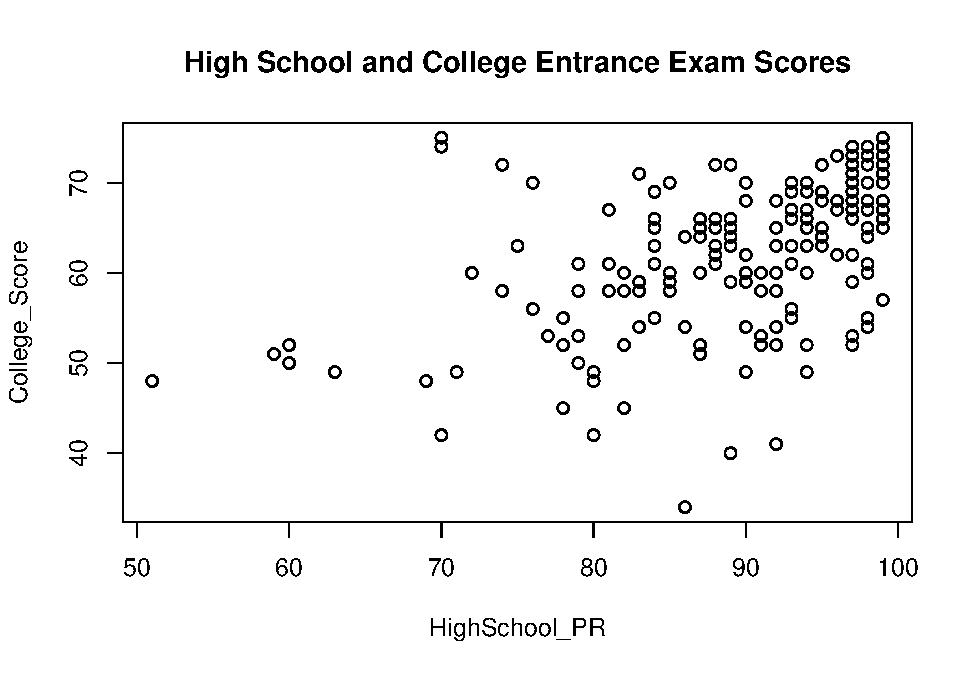
\includegraphics{PTT_Analysis_of_Test_Scores_Unfinished_files/figure-latex/bivariate-1.pdf}

We use the correlation coefficient to measure the strength of the linear
relationship between \textbf{HighSchool\_PR} and
\textbf{College\_Score}. The computed value is approximately 0.507,
showing a medium strength of positive association between the two
variables. We can interpret that a better score in the high school
entrance exam is associated with a better college entrance exam score,
but the relationship is not as strong after \textbf{HighSchool\_PR}
reaches 80. (Note that correlation does not imply causality!)

\begin{Shaded}
\begin{Highlighting}[]
\FunctionTok{cor}\NormalTok{(data\_corr}\SpecialCharTok{$}\NormalTok{HighSchool\_PR, data\_corr}\SpecialCharTok{$}\NormalTok{College\_Score)}
\end{Highlighting}
\end{Shaded}

\begin{verbatim}
## [1] 0.5074473
\end{verbatim}

To find the correlation coefficient between the random variables
\(X, Y\), we start with the covariance \(\text{Cov}(X,Y)\) in the
equation below. \(E[X]\) denotes the expectation value of \(X\), a.k.a.
the mean of \(X\).

\[\text{Cov}(X,Y) = E[(X-E[X])(Y-E[Y])] = E[XY] - E[X]E[Y].\]

Then we also need to compute the standard deviation \(\sigma_X\):

\[\sigma_X = \sqrt{E[(X-E[X])^2]} = \sqrt{E[X^2]-(E[X])^2}.\] Similarly,
the standard deviation \(\sigma_Y\) is:

\[\sigma_Y = \sqrt{E[(Y-E[Y])^2]} = \sqrt{E[Y^2]-(E[Y])^2}.\]

Finally, we can calculate the correlation coefficient as:

\[\rho_{X,Y} = \dfrac{\text{Cov}(X,Y)}{\sigma_X \sigma_Y}.\]

The correlation coefficient \(\rho\) is always between -1 and +1. The
stronger \(|\rho_{X,Y}|\) is, the stronger is the linear relationship. A
positive value means the two variables \(X,Y\) are positively associated
with each other. In other words, when \(X\) increases, \(Y\) is also
expected to increase. A negative value means the two variables \(X,Y\)
are negatively associated with each other. In this case, when \(X\)
increases, \(Y\) is expected to decrease. The correlation coefficient
may be zero, but this simply means that \(X\) and \(Y\) do not have a
linear relationship with each other. There may exist other patterns
between the two variables.

The strength of linear relationship can be interpreted as
below:\footnote{\url{https://bit.ly/3AUI8PA}}

\begin{itemize}
\item
  \(|\rho| = 1\): Perfect linear relationship
\item
  \(0.6 < |\rho| < 1\): Strong linear relationship
\item
  \(0.4 < |\rho| < 0.6\): Moderate linear relationship
\item
  \(0.2 < |\rho| < 0.4\): Low linear relationship
\item
  \(0 < |\rho| < 0.2\): Little-to-no linear relationship
\item
  \(|\rho| = 0\): No linear relationship
\end{itemize}

\hypertarget{examples-of-the-correlation-coefficient}{%
\subsubsection{Examples of the Correlation
Coefficient}\label{examples-of-the-correlation-coefficient}}

Here we visualize some bivariate patterns for different values of the
correlation coefficient \(\rho\), with hypothetical data and examples.
The graph ideas came from \emph{OpenIntro Statistics}
\citep{diez2019openintro}. We hide the code that generated these graphs
to avoid obscuring the topic, and the interested readers can find the
code in the raw \texttt{.Rmd} files. We will discuss more about linear
regression in Chapter \ref{linear-reg}.

The first row of graphs show what \(|\rho| = 1\) looks like -- a
straight line, i.e., a perfect linear relationship. In mathematical
terms, we can write \(Y = \alpha + \beta X\), where the sign of
\(\beta\) controls the direction of the pattern.

\begin{itemize}
\item
  For \(\rho = 1\), the two variables \(X, Y\) have a perfect positive
  linear relationship (\(\beta > 0\)). One example is people's height in
  cm and height in inches, where the two variables are a positive linear
  combination of each other.
\item
  For \(\rho = -1\), the two variables \(X, Y\) have a perfect negative
  linear relationship (\(\beta < 0\)). One example is you eat from a box
  of 12 cookies. The cookies you ate and the cookies remaining should
  add up to 12, so they have a perfect negative linear relationship.
\end{itemize}

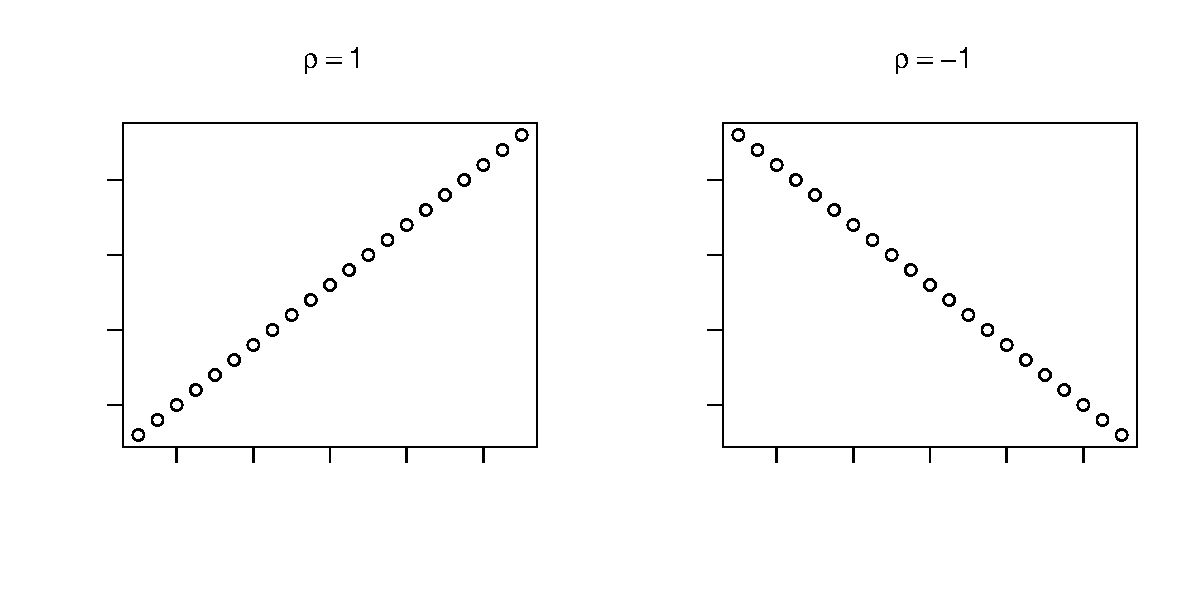
\includegraphics{PTT_Analysis_of_Test_Scores_Unfinished_files/figure-latex/perfect-linear-correlation-1.pdf}

In the second row, the two variables in each plot have a good but
imperfect linear relationship. The datapoints seem to be on a straight
line with some fluctuation. If we start with the linear equation, we can
add a small random noise with mean zero to the data generative process.
Hence the equation becomes \(Y = \alpha + \beta X + \epsilon\), where
\(\epsilon \sim N(0,\sigma^2)\). We assume the random noise \(\epsilon\)
follows a normal distribution, although this is not always necessary.

\begin{itemize}
\item
  The left graph illustrates \(\rho = 0.89\). The plot shows a clear and
  positive relationship with some noise. One example is the height and
  weight of children of various ages. Taller children usually weigh
  more, but this is not always the case. (Childhood obesity is a serious
  health problem.)
\item
  The right graph illustrates \(\rho = -0.93\). The plot shows a clear
  and negative relationship with some noise. One example is the hours
  for work and the hours for hobbies. Generally, the more time you spend
  on work, the less time you spend on hobbies. Although everyone has 24
  hours in a day, the time outside work does not always mean you are
  spending on hobbies for enjoyment.
\end{itemize}

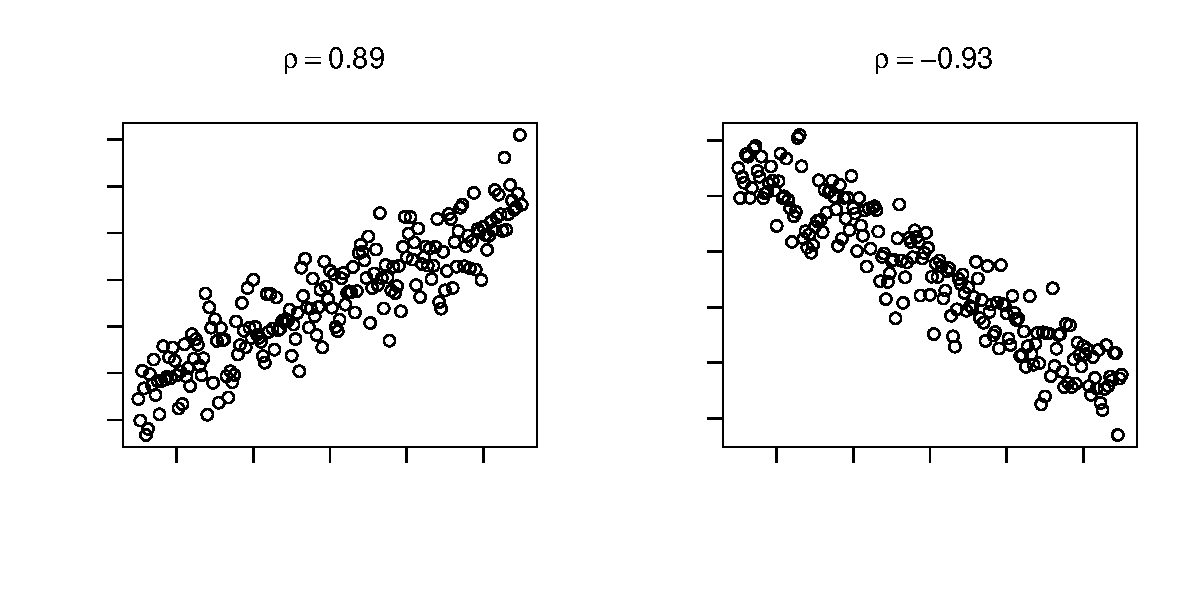
\includegraphics{PTT_Analysis_of_Test_Scores_Unfinished_files/figure-latex/high-correlation-1.pdf}

The third row contains graphs that visualize a medium level of linear
correlation, where \(0.4 < |\rho| < 0.6\). The linear trend is still
visible, but with more fluctuation than in the high-correlation graphs.

\begin{itemize}
\item
  The left figure shows \(\rho = 0.64\), as a positive medium
  correlation of the two variables. One example is students' midterm
  exam scores and final exam scores. Students who did well on the
  midterm often continue to do well on the final, but this is not
  guaranteed. Exam scores often have more variability than people's
  height and weight.
\item
  The right figure shows \(\rho = -0.47\), as a negative medium
  correlation of the two variables. One example is adults' muscle mass
  and their age. Older adults tend to have less muscle than younger
  ones, but it is well-known that strength training helps preserve some
  muscle mass.\footnote{We are not medical professionals, so we make the
    caveat that the linear relationship may not be accurate.}
\end{itemize}

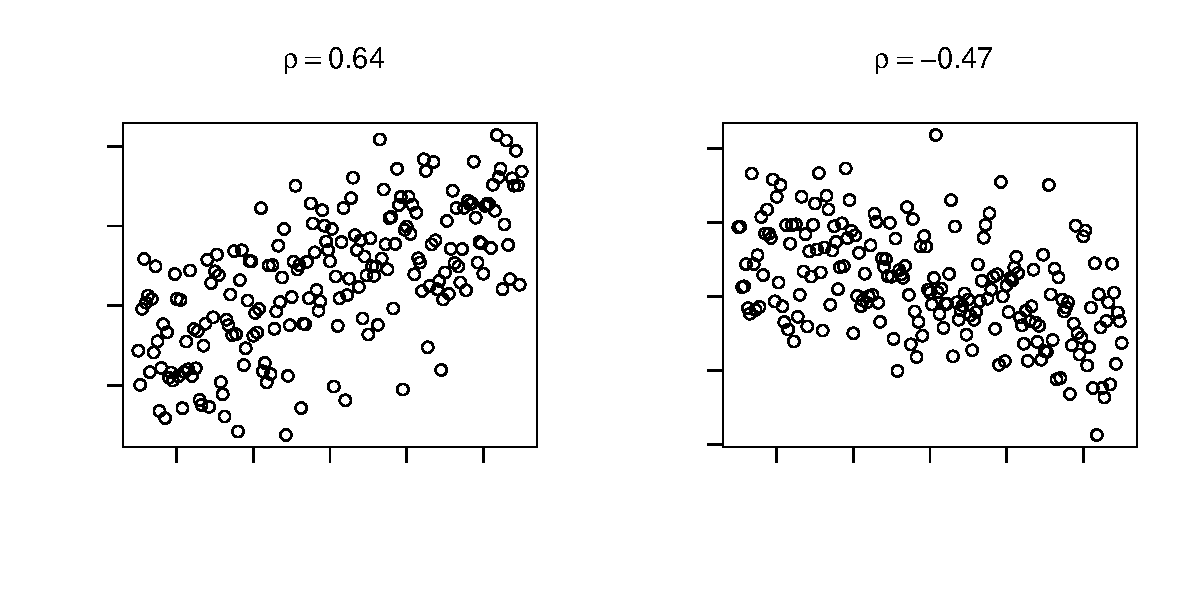
\includegraphics{PTT_Analysis_of_Test_Scores_Unfinished_files/figure-latex/mid-correlation-1.pdf}

The final row shows what little-to-no linear correlation looks like. We
need to remember that zero correlation does not mean the two variables
are independent. They may have a non-linear relationship, which cannot
be detected by the correlation coefficient.

\begin{itemize}
\item
  The left image shows a bivariate scatter plot with \(\rho = 0.03\),
  i.e., very little correlation. For a small \(\rho\) in absolute value,
  the two variables barely have any linear relationship. Although the
  bivariate scatter plot looks random, the correlation coefficient may
  not be exactly zero. One example is the daily coffee consumption and
  intelligence (IQ scores). How much coffee an individual drinks is
  completely unrelated to his/her intelligence level, so we cannot use
  one variable to obtain information of the other.\footnote{\url{https://www.statology.org/no-correlation-examples/}}
\item
  The right image has \(\rho = 0\) (absolute zero), i.e., no linear
  relationship at all. However, the graph shows a parabola curve, so the
  two variables have some non-linear relationship. If you throw a ball
  to another person, the ball's trajectory would look like a
  parabola.\footnote{\url{https://www.wondriumdaily.com/mathematics-of-falling-the-parabolic-movement/}}
  The x-axis is horizontal and parallel to the ground, while the y-axis
  is vertical and perpendicular to the x-axis.
\end{itemize}

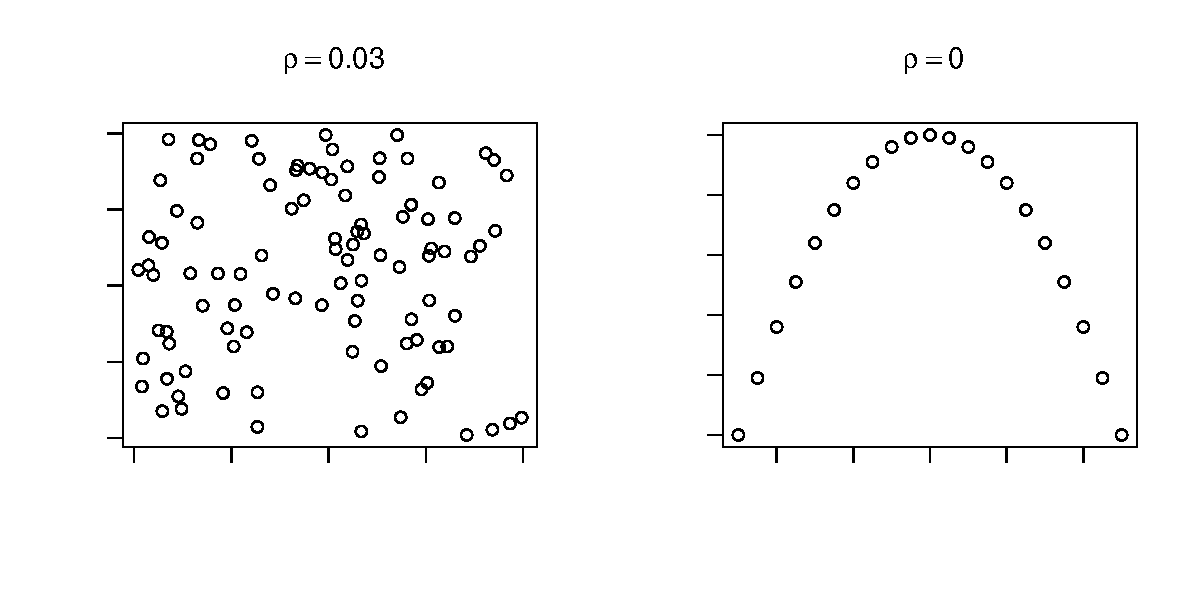
\includegraphics{PTT_Analysis_of_Test_Scores_Unfinished_files/figure-latex/low-correlation-1.pdf}

\hypertarget{linear-reg}{%
\section{Linear Regression}\label{linear-reg}}

Linear regression is a commonly-used statistical model to evaluate the
relationship between two continuous variables, and even major companies
like IBM endorse linear regression for better decision-making in
business.\footnote{\url{https://www.ibm.com/topics/linear-regression}}
Therefore, we are going to decide whether we should run a linear
regression to predict \textbf{College\_Score} from
\textbf{HighSchool\_PR}. If yes, we would implement the model and check
the residuals. If no, we need to explore other options in analyzing the
data.

A linear regression model can be written in mathematical terms:

\[Y = \alpha + \beta X + \epsilon\]

\(Y\) is the response variable, i.e., what we would like to predict.
\(X\) is the explanatory variable, i.e., the data used to make the
predictions. \(\alpha\) is the intercept, and it stands for the estimate
\(\hat{Y}\) when \(X = 0\) (if applicable). \(\beta\) is the
coefficient, and when \(X\) increases by one unit, we can expect \(Y\)
to increase by \(\beta\) units. Last but not least, \(\epsilon\) is the
error term, which is normally distributed with mean zero.

\emph{OpenIntro Statistics} \citep{diez2019openintro} states that four
requirements need to be met in a linear regression:

\begin{enumerate}
\item \textbf{Linearity}: The data has a linear trend, not a curve.
\item \textbf{Nearly normal residuals}: The residuals should be nearly normal, and we need to beware of outliers and influential points.
\item \textbf{Constant variability}: The variability of $Y$ is constant and does not depend on the value of $X$.
\item \textbf{Independent observations}: Each observation (datapoint) is independent of the others.
\end{enumerate}

\hypertarget{should-we-run-a-linear-regression}{%
\subsection{Should we run a linear
regression?}\label{should-we-run-a-linear-regression}}

It is inappropriate to perform linear regression directly, because the
data do not meet the constant variability assumption. In the bivariate
exploratory plot, we can see that the variability of
\textbf{College\_Score} (\(Y\)) increases as \textbf{HighSchool\_PR}
(\(X\)) increases. One possible remedy is apply the square root
transformation to \textbf{College\_Score}, in order to reduce the
variability. But the scatterplot below shows little to no improvement in
variability, and the correlation coefficient even drops from 0.507 to
0.504. Hence we determine that it is not a good idea to run a linear
regression model on the whole dataset.

\begin{Shaded}
\begin{Highlighting}[]
\CommentTok{\# data version: already removed missing data}
\CommentTok{\# data\_corr = data[{-}missing\_rows,]}

\FunctionTok{plot}\NormalTok{(data\_corr}\SpecialCharTok{$}\NormalTok{HighSchool\_PR, }\FunctionTok{sqrt}\NormalTok{(data\_corr}\SpecialCharTok{$}\NormalTok{College\_Score),}
     \AttributeTok{main =} \StringTok{"High School and College Entrance Exam Scores"}\NormalTok{,}
     \AttributeTok{xlab=}\StringTok{"HighSchool\_PR"}\NormalTok{,}
     \AttributeTok{ylab=}\StringTok{"Square Root of College\_Score"}\NormalTok{)}
\end{Highlighting}
\end{Shaded}

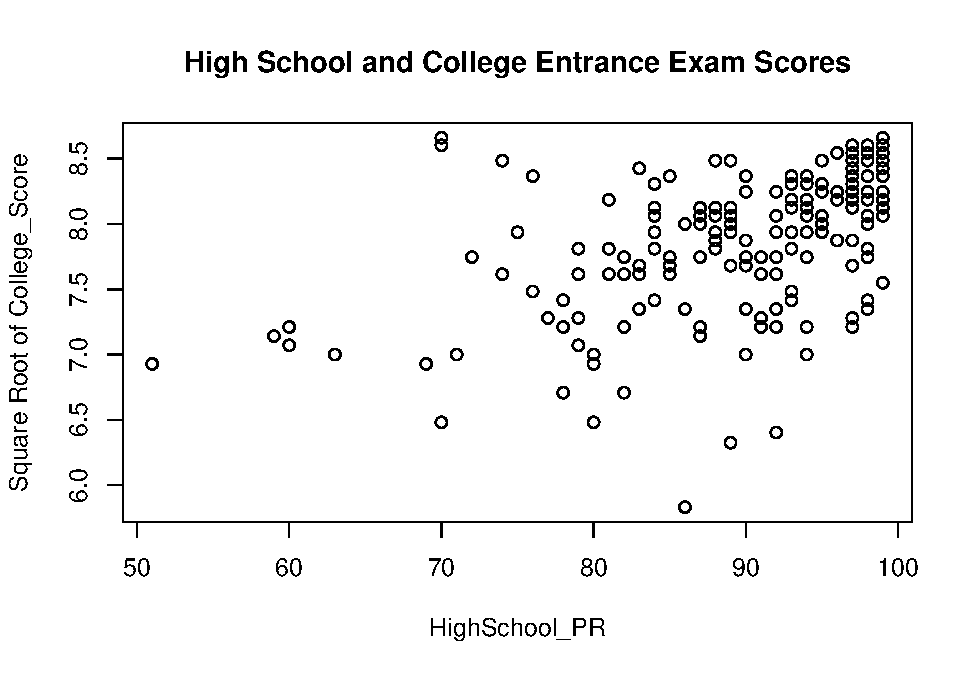
\includegraphics{PTT_Analysis_of_Test_Scores_Unfinished_files/figure-latex/transform-test-1.pdf}

\begin{Shaded}
\begin{Highlighting}[]
\FunctionTok{cor}\NormalTok{(data\_corr}\SpecialCharTok{$}\NormalTok{HighSchool\_PR, }\FunctionTok{sqrt}\NormalTok{(data\_corr}\SpecialCharTok{$}\NormalTok{College\_Score))}
\end{Highlighting}
\end{Shaded}

\begin{verbatim}
## [1] 0.5048132
\end{verbatim}

\hypertarget{examine-further}{%
\subsection{Segmenting the Data}\label{examine-further}}

Instead, we should segment the data and further examine the top scorers
in the dataset, i.e., those with \textbf{HighSchool\_PR} 80 or higher.
Most of these respondents have \textbf{College\_Score} of 60 or higher,
but the range of \textbf{College\_Score} is wide. Here, we add
horizontal and vertical lines to clarify the graph.

\begin{Shaded}
\begin{Highlighting}[]
\FunctionTok{plot}\NormalTok{(data\_corr}\SpecialCharTok{$}\NormalTok{HighSchool\_PR, data\_corr}\SpecialCharTok{$}\NormalTok{College\_Score,}
     \AttributeTok{main =} \StringTok{"High School and College Entrance Exam Scores"}\NormalTok{,}
     \AttributeTok{xlab=}\StringTok{"HighSchool\_PR"}\NormalTok{,}
     \AttributeTok{ylab=}\StringTok{"College\_Score"}\NormalTok{)}

\FunctionTok{abline}\NormalTok{(}\AttributeTok{h=}\DecValTok{60}\NormalTok{,}\AttributeTok{v=}\DecValTok{80}\NormalTok{)}
\end{Highlighting}
\end{Shaded}

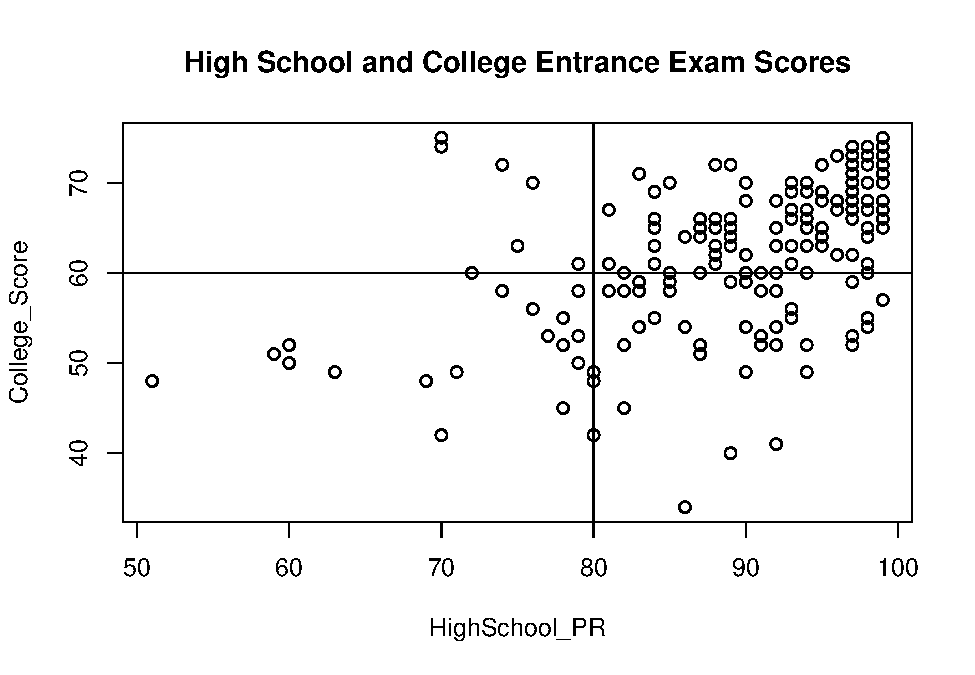
\includegraphics{PTT_Analysis_of_Test_Scores_Unfinished_files/figure-latex/high-scorer-obs-1.pdf}

We can also create a contingency table (a.k.a. cross tabulation) for the
two indicators \textbf{HighSchool\_80up} and \textbf{College\_60up},
which displays the bivariate frequency distribution in terms of counts.

\begin{itemize}
\tightlist
\item
  \textbf{HighSchool\_80up}: Indicator of whether
  \textbf{HighSchool\_PR} is 80 or higher
\item
  \textbf{College\_60up}: Indicator of whether \textbf{College\_Score}
  is 60 or higher
\end{itemize}

\begin{Shaded}
\begin{Highlighting}[]
\NormalTok{data\_corr}\SpecialCharTok{$}\NormalTok{HS\_80up }\OtherTok{=}\NormalTok{ data\_corr}\SpecialCharTok{$}\NormalTok{HighSchool\_PR }\SpecialCharTok{\textgreater{}=} \DecValTok{80}
\NormalTok{data\_corr}\SpecialCharTok{$}\NormalTok{CS\_60up }\OtherTok{=}\NormalTok{ data\_corr}\SpecialCharTok{$}\NormalTok{College\_Score }\SpecialCharTok{\textgreater{}=}\DecValTok{60}

\NormalTok{contingency }\OtherTok{=} \FunctionTok{table}\NormalTok{(data\_corr}\SpecialCharTok{$}\NormalTok{HS\_80up, data\_corr}\SpecialCharTok{$}\NormalTok{CS\_60up,}
                    \AttributeTok{dnn=}\FunctionTok{c}\NormalTok{(}\StringTok{"HighSchool\_80up"}\NormalTok{,}\StringTok{"College\_60up"}\NormalTok{))}

\NormalTok{contingency}
\end{Highlighting}
\end{Shaded}

\begin{verbatim}
##                College_60up
## HighSchool_80up FALSE TRUE
##           FALSE    17    8
##           TRUE     43  120
\end{verbatim}

To make the table easier to read, we revert the order of \texttt{FALSE}
and \texttt{TRUE} in the contingency table by calling the indices in
reverse order.

\begin{Shaded}
\begin{Highlighting}[]
\NormalTok{contingency }\OtherTok{=}\NormalTok{ contingency[}\DecValTok{2}\SpecialCharTok{:}\DecValTok{1}\NormalTok{, }\DecValTok{2}\SpecialCharTok{:}\DecValTok{1}\NormalTok{]}
\NormalTok{contingency}
\end{Highlighting}
\end{Shaded}

\begin{verbatim}
##                College_60up
## HighSchool_80up TRUE FALSE
##           TRUE   120    43
##           FALSE    8    17
\end{verbatim}

Below is the percentage version of the contingency table, and we can see
that more than 63.5\% of the respondents have both
\textbf{HighSchool\_PR} \(\geq\) 80 and \textbf{College\_Score} \(\geq\)
60. This is also evidence that the PTT users tend to come from the
population who scored well on the high school and college entrance
exams.

\begin{Shaded}
\begin{Highlighting}[]
\FunctionTok{prop.table}\NormalTok{(contingency)}
\end{Highlighting}
\end{Shaded}

\begin{verbatim}
##                College_60up
## HighSchool_80up       TRUE      FALSE
##           TRUE  0.63829787 0.22872340
##           FALSE 0.04255319 0.09042553
\end{verbatim}

We can also round the percentage version to four decimal places in the
ratio, so we will have two decimal places after the integer percentage.
For example, 0.4528 becomes 45.28\%.

\begin{Shaded}
\begin{Highlighting}[]
\FunctionTok{round}\NormalTok{(}\FunctionTok{prop.table}\NormalTok{(contingency),}\DecValTok{4}\NormalTok{)}
\end{Highlighting}
\end{Shaded}

\begin{verbatim}
##                College_60up
## HighSchool_80up   TRUE  FALSE
##           TRUE  0.6383 0.2287
##           FALSE 0.0426 0.0904
\end{verbatim}

\hypertarget{conditional-probability}{%
\subsection{Conditional Probability}\label{conditional-probability}}

Using conditional probability, we can answer this question from the
data: If a person scores at least 80 on the high school entrance score
percentile rank (PR), how likely is he/she going to obtain a score at
least 60 on the college entrance exam?

In mathematical terms, this is equivalent to finding
\(P(\text{College$\_$60up is true } \vert \text{ HighSchool$\_$80up is true})\).
Recall the conditional probability formula and the Bayes theorem:

\[P(A|B) = \frac{P(A \cap B)}{P(B)} = \frac{P(B|A)P(A)}{P(B)}\]

In this data, we have

\begin{itemize}
\item
  \(P(\text{HighSchool$\_$80up is true})\) = \# of respondents with
  \textbf{HighSchool\_PR} \(\geq\) 80 / all respondents.
\item
  \(P(\text{College$\_$60up is true})\) = \# of respondents with
  \textbf{College\_Score} \(\geq\) 60 / all respondents.
\item
  \(P(\text{HighSchool$\_$80up is true} \cap \text{College$\_$60up is true})\)\\
  = \# of respondents with \textbf{HighSchool\_PR} \(\geq\) 80 and
  \textbf{College\_Score} \(\geq\) 60 / all respondents.
\end{itemize}

Plugging the numbers into the equation, we get

\[\begin{aligned} 
& P(\text{College$\_$60up is true } \vert \text{ HighSchool$\_$80up is true})\\
&= \frac{P(\text{HighSchool$\_$80up is true} \cap \text{College$\_$60up is true})}{P(\text{HighSchool$\_$80up is true})} \\
&= \frac{\text{$\#$ of respondents with HighSchool$\_$PR $\geq$ 80 and College$\_$Score $\geq$ 60}}{\text{$\#$ of respondents with HighSchool$\_$PR $\geq$ 80}} \\
&= \frac{120}{43+120} \approx 0.7362.
\end{aligned}\]

According to this data from PTT, there is a 73.62\% chance for a person
to score at least 60 on the college entrance exam, given that he/she
scored at least 80 on the high school entrance score percentile rank
(PR). Note that we use number of respondents rather than percentage to
avoid rounding errors.

In comparison, if we do not know anything about the person's high school
entrance score percentile rank (PR), we have a probability of 63.82\% in
observing the person scoring at least 60 on the college entrance exam.
There is an increase of 9.80\% in probability after we learn information
about his/her high school entrance exam score.

\[\begin{aligned}
P(\text{College$\_$60up is true}) &= \text{$\#$ of respondents with College$\_$Score $\geq$ 60 / all respondents} \\
&= \frac{120}{188} \approx 0.6382.
\end{aligned}\]

\begin{Shaded}
\begin{Highlighting}[]
\FunctionTok{nrow}\NormalTok{(data\_corr) }\CommentTok{\# number of all respondents without missing data}
\end{Highlighting}
\end{Shaded}

\begin{verbatim}
## [1] 188
\end{verbatim}

\textbf{Remark}: Conditional probability is the foundation of Bayesian
statistics, which updates the existing probabilities given the new data.
For the interested readers, we recommend the book
\textit{An Introduction to Bayesian Thinking}
\citep{clyde2018bayesian101} as a start. This book was written as a
companion for the Bayesian Statistics course on Coursera from Duke
University.\footnote{\url{https://www.coursera.org/learn/bayesian}}
Knowledge of calculus is helpful but not an absolute prerequisite.

\hypertarget{explore-top}{%
\section{Top Scorers: A Closer Look}\label{explore-top}}

We would like to further examine the top scorers, given the high number
of records in the data observed in Section \ref{examine-further}. In
Taiwan's education system, the top tier of high schools and colleges can
be further segmented. The top of the range can be very different than
the middle or bottom. For example, National Taiwan University\footnote{\url{https://www.ntu.edu.tw/english/}}
is the most prestigious university in Taiwan, but Chang Gung
University\footnote{\url{https://www.cgu.edu.tw/?Lang=en}} is also
excellent in medical education. However, many people in the US have
heard of the former but not the latter. This does not mean you should
always choose the most prestigious college; many other factors should
also be considered, such as tuition and majors offered at that college.

We consider the following subcategories in the entrance exam scores:

\begin{itemize}
\tightlist
\item
  \textbf{HighSchool\_PR} ranges: 80-89, 90-94, 95-99
\item
  \textbf{College\_Score} ranges: 60-64, 65-69, 70-75
\end{itemize}

Let's investigate the univariate distributions of
\textbf{HighSchool\_PR} and \textbf{College\_Score} respectively, then
we move on to explore the bivariate relationship between the two sets of
scores. It is good practice to start with one variable at a time, even
when we are mainly interested in the relationship between the two
variables.

\hypertarget{HighSchool-PR-80-up}{%
\subsection{High School Entrance Exam Scores (Percentile Rank) at least
80}\label{HighSchool-PR-80-up}}

We use the \texttt{R} function \texttt{table} to show the frequency of
each \textbf{HighSchool\_PR} value that is at least 80, and we have 163
values in total. In the table below, the first row is the PR (percentile
rank), and the second row is the counts. Although we truncated the
\textbf{HighSchool\_PR} to 80 and above, the distribution is still
left-skewed. The \textbf{HighSchool\_PR} 99 has the highest counts,
followed by \textbf{HighSchool\_PR} 97 and \textbf{HighSchool\_PR} 98.

\begin{Shaded}
\begin{Highlighting}[]
\NormalTok{HS\_PR\_seg }\OtherTok{=}\NormalTok{ data\_corr}\SpecialCharTok{$}\NormalTok{HighSchool\_PR[}\FunctionTok{which}\NormalTok{(data\_corr}\SpecialCharTok{$}\NormalTok{HS\_80up }\SpecialCharTok{==} \ConstantTok{TRUE}\NormalTok{)]}
\FunctionTok{length}\NormalTok{(HS\_PR\_seg)}
\end{Highlighting}
\end{Shaded}

\begin{verbatim}
## [1] 163
\end{verbatim}

\begin{Shaded}
\begin{Highlighting}[]
\FunctionTok{table}\NormalTok{(HS\_PR\_seg)}
\end{Highlighting}
\end{Shaded}

\begin{verbatim}
## HS_PR_seg
## 80 81 82 83 84 85 86 87 88 89 90 91 92 93 94 95 96 97 98 99 
##  3  4  4  4  6  4  3  7  6  8  7  6  9 11 11  7  5 18 15 25
\end{verbatim}

Or if you prefer a histogram, we can also create one.

\begin{Shaded}
\begin{Highlighting}[]
\FunctionTok{hist}\NormalTok{(HS\_PR\_seg, }\AttributeTok{xlab=}\StringTok{"HighSchool\_PR"}\NormalTok{,}
     \AttributeTok{main=}\StringTok{"Histogram of HighSchool\_PR 80 and above"}\NormalTok{)}
\end{Highlighting}
\end{Shaded}

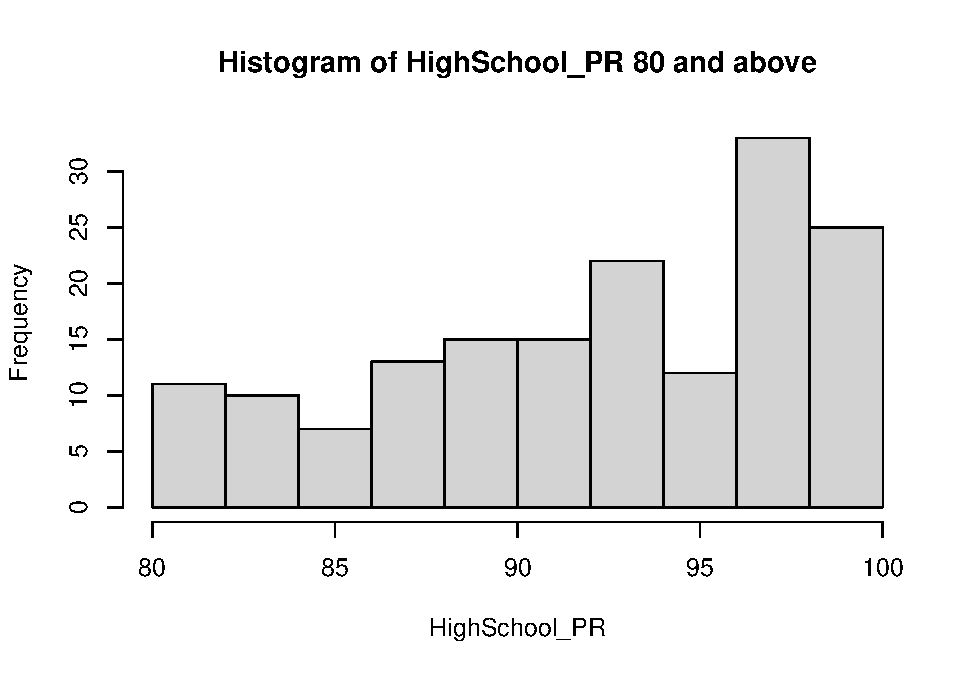
\includegraphics{PTT_Analysis_of_Test_Scores_Unfinished_files/figure-latex/high-school-pr-seg-hist-1.pdf}

Therefore, we create the breakdown of the \textbf{HighSchool\_PR}
ranges: 80-89, 90-94, 95-99. There are 49 records in the 80-89 range, 44
records in 90-94, and 70 records in 95-99. We divided the 90-99 range
into 90-94 and 95-99, but the number of \textbf{HighSchool\_PR} records
in the 95-99 range is still higher than any of the other two categories.

However, it is not a good idea to further divide the 95-99 range into
95-97 and 98-99, due to the lack of geographic information. In Taipei,
the high school enrollment is extremely competitive. Students with
\textbf{HighSchool\_PR} 95 and those with \textbf{HighSchool\_PR} 99
would get admitted to high schools of different rankings.\footnote{\url{https://w199584.pixnet.net/blog/post/28321887}}
But in other parts of Taiwan, most students with \textbf{HighSchool\_PR}
at least 95 would already qualify for the top local high school, and
some rural parts even require a lower \textbf{HighSchool\_PR} to get
into the county's top high school.

\begin{Shaded}
\begin{Highlighting}[]
\NormalTok{HS80to89 }\OtherTok{=} \FunctionTok{length}\NormalTok{(}\FunctionTok{which}\NormalTok{(HS\_PR\_seg }\SpecialCharTok{\textgreater{}=} \DecValTok{80} \SpecialCharTok{\&}\NormalTok{ HS\_PR\_seg }\SpecialCharTok{\textless{}=} \DecValTok{89}\NormalTok{))}
\NormalTok{HS90to94 }\OtherTok{=} \FunctionTok{length}\NormalTok{(}\FunctionTok{which}\NormalTok{(HS\_PR\_seg }\SpecialCharTok{\textgreater{}=} \DecValTok{90} \SpecialCharTok{\&}\NormalTok{ HS\_PR\_seg }\SpecialCharTok{\textless{}=} \DecValTok{94}\NormalTok{))}
\NormalTok{HS95to99 }\OtherTok{=} \FunctionTok{length}\NormalTok{(}\FunctionTok{which}\NormalTok{(HS\_PR\_seg }\SpecialCharTok{\textgreater{}=} \DecValTok{95} \SpecialCharTok{\&}\NormalTok{ HS\_PR\_seg }\SpecialCharTok{\textless{}=} \DecValTok{99}\NormalTok{))}
\end{Highlighting}
\end{Shaded}

\begin{Shaded}
\begin{Highlighting}[]
\FunctionTok{print}\NormalTok{(}\FunctionTok{paste}\NormalTok{(}\StringTok{"HighSchool\_PR 80{-}89:"}\NormalTok{,HS80to89))}
\end{Highlighting}
\end{Shaded}

\begin{verbatim}
## [1] "HighSchool_PR 80-89: 49"
\end{verbatim}

\begin{Shaded}
\begin{Highlighting}[]
\FunctionTok{print}\NormalTok{(}\FunctionTok{paste}\NormalTok{(}\StringTok{"HighSchool\_PR 90{-}94:"}\NormalTok{,HS90to94))}
\end{Highlighting}
\end{Shaded}

\begin{verbatim}
## [1] "HighSchool_PR 90-94: 44"
\end{verbatim}

\begin{Shaded}
\begin{Highlighting}[]
\FunctionTok{print}\NormalTok{(}\FunctionTok{paste}\NormalTok{(}\StringTok{"HighSchool\_PR 95{-}99:"}\NormalTok{,HS95to99))}
\end{Highlighting}
\end{Shaded}

\begin{verbatim}
## [1] "HighSchool_PR 95-99: 70"
\end{verbatim}

\hypertarget{college-60-up}{%
\subsection{College Entrance Exam Scores at least
60}\label{college-60-up}}

Similar to the previous section, we also show the frequency of each
\textbf{College\_Score} value that is at least 60. The total counts is
128, fewer than the 163 counts with \textbf{HighSchool\_PR} 80 or above.
The distribution is relatively uniform for \textbf{College\_Score}
values between 60 and 73, with a steep decline in the counts of
\textbf{College\_Score} 74 and 75 (max possible score). On the college
entrance exam, only four respondents scored 74 and two scored 75.
According to the historical statistics of the college entrance exam in
Taiwan, \textbf{College\_Score} 74 and 75 account for approximately
0.2\% of all test takers each year, which is quite a small percentage.

\begin{Shaded}
\begin{Highlighting}[]
\NormalTok{CS\_Score\_seg }\OtherTok{=}\NormalTok{ data\_corr}\SpecialCharTok{$}\NormalTok{College\_Score[}\FunctionTok{which}\NormalTok{(data\_corr}\SpecialCharTok{$}\NormalTok{CS\_60up }\SpecialCharTok{==} \ConstantTok{TRUE}\NormalTok{)]}
\FunctionTok{length}\NormalTok{(CS\_Score\_seg)}
\end{Highlighting}
\end{Shaded}

\begin{verbatim}
## [1] 128
\end{verbatim}

\begin{Shaded}
\begin{Highlighting}[]
\FunctionTok{table}\NormalTok{(CS\_Score\_seg)}
\end{Highlighting}
\end{Shaded}

\begin{verbatim}
## CS_Score_seg
## 60 61 62 63 64 65 66 67 68 69 70 71 72 73 74 75 
## 10  7  4 10  5 11 12  9  9  6 10  9 12  8  4  2
\end{verbatim}

Before we display the histogram, let's create a table to (approximately)
convert \textbf{College\_Score} into PR (Percentile Rank) using
2001-2014 data.\footnote{\url{https://web.archive.org/web/20150207042900/http://www.ceec.edu.tw/AbilityExam/AbilityExamStat.htm}}
This gives readers an understanding of what percentage of test takers
(high school students in grade 12) get what scores. For example, a
\textbf{College\_Score} of 70 would be at the 98.5th percentile, i.e.,
PR 98.5.

\begin{Shaded}
\begin{Highlighting}[]
\NormalTok{college\_score }\OtherTok{=} \FunctionTok{c}\NormalTok{(}\DecValTok{60}\NormalTok{,}\DecValTok{65}\NormalTok{,}\DecValTok{70}\NormalTok{,}\DecValTok{74}\NormalTok{,}\DecValTok{75}\NormalTok{)}
\NormalTok{college\_pr }\OtherTok{=} \FunctionTok{c}\NormalTok{(}\DecValTok{88}\NormalTok{, }\DecValTok{95}\NormalTok{, }\FloatTok{98.5}\NormalTok{, }\FloatTok{99.9}\NormalTok{, }\DecValTok{100}\NormalTok{)}

\FunctionTok{data.frame}\NormalTok{(college\_score, college\_pr)}
\end{Highlighting}
\end{Shaded}

\begin{verbatim}
##   college_score college_pr
## 1            60       88.0
## 2            65       95.0
## 3            70       98.5
## 4            74       99.9
## 5            75      100.0
\end{verbatim}

Here is the histogram of the \textbf{College\_Score} values 60 and
above.

\begin{Shaded}
\begin{Highlighting}[]
\FunctionTok{hist}\NormalTok{(CS\_Score\_seg, }\AttributeTok{xlab=}\StringTok{"College\_Score (max possible is 75)"}\NormalTok{,}
     \AttributeTok{main=}\StringTok{"Histogram of College\_Score 60 and above"}\NormalTok{)}
\end{Highlighting}
\end{Shaded}

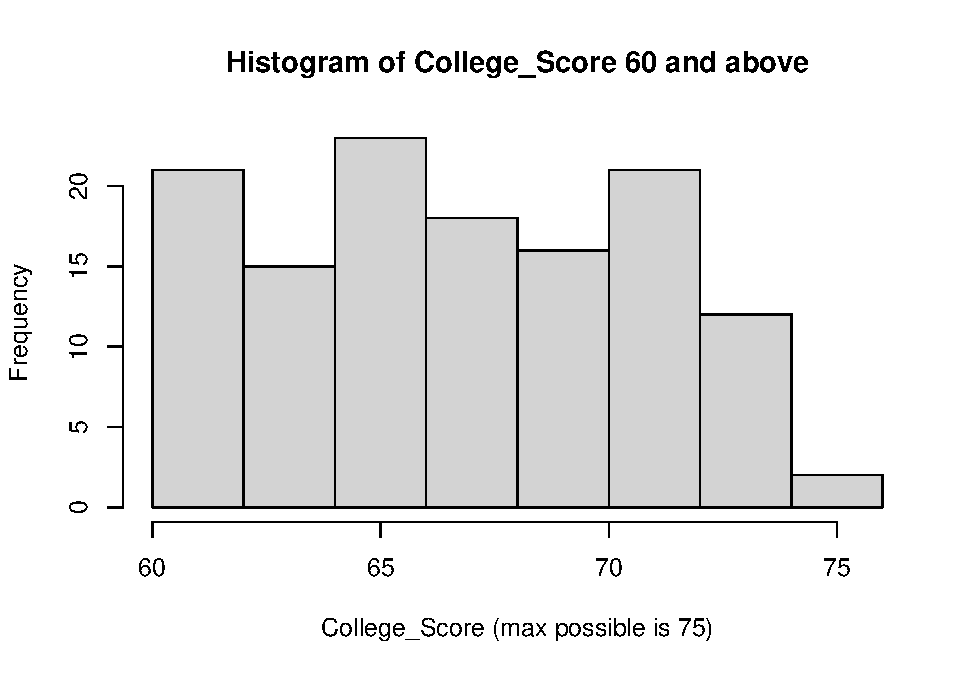
\includegraphics{PTT_Analysis_of_Test_Scores_Unfinished_files/figure-latex/college-score-seg-hist-1.pdf}

We also create the breakdown of the \textbf{College\_Score} ranges:
60-64, 65-69, 70-75. There are 36 records in the 60-64 range, 47 records
in 65-69, and 45 records in 70-75. This is also relatively more uniform
than the \textbf{HighSchool\_PR} breakdown (49, 44, and 70 records
each).

\begin{Shaded}
\begin{Highlighting}[]
\NormalTok{CS60to64 }\OtherTok{=} \FunctionTok{length}\NormalTok{(}\FunctionTok{which}\NormalTok{(CS\_Score\_seg }\SpecialCharTok{\textgreater{}=} \DecValTok{60} \SpecialCharTok{\&}\NormalTok{ CS\_Score\_seg }\SpecialCharTok{\textless{}=} \DecValTok{64}\NormalTok{))}
\NormalTok{CS65to69 }\OtherTok{=} \FunctionTok{length}\NormalTok{(}\FunctionTok{which}\NormalTok{(CS\_Score\_seg }\SpecialCharTok{\textgreater{}=} \DecValTok{65} \SpecialCharTok{\&}\NormalTok{ CS\_Score\_seg }\SpecialCharTok{\textless{}=} \DecValTok{69}\NormalTok{))}
\NormalTok{CS70to75 }\OtherTok{=} \FunctionTok{length}\NormalTok{(}\FunctionTok{which}\NormalTok{(CS\_Score\_seg }\SpecialCharTok{\textgreater{}=} \DecValTok{70} \SpecialCharTok{\&}\NormalTok{ CS\_Score\_seg }\SpecialCharTok{\textless{}=} \DecValTok{75}\NormalTok{))}
\end{Highlighting}
\end{Shaded}

\begin{Shaded}
\begin{Highlighting}[]
\FunctionTok{print}\NormalTok{(}\FunctionTok{paste}\NormalTok{(}\StringTok{"College\_Score 60{-}64:"}\NormalTok{,CS60to64))}
\end{Highlighting}
\end{Shaded}

\begin{verbatim}
## [1] "College_Score 60-64: 36"
\end{verbatim}

\begin{Shaded}
\begin{Highlighting}[]
\FunctionTok{print}\NormalTok{(}\FunctionTok{paste}\NormalTok{(}\StringTok{"College\_Score 65{-}69:"}\NormalTok{,CS65to69))}
\end{Highlighting}
\end{Shaded}

\begin{verbatim}
## [1] "College_Score 65-69: 47"
\end{verbatim}

\begin{Shaded}
\begin{Highlighting}[]
\FunctionTok{print}\NormalTok{(}\FunctionTok{paste}\NormalTok{(}\StringTok{"College\_Score 70{-}75:"}\NormalTok{,CS70to75))}
\end{Highlighting}
\end{Shaded}

\begin{verbatim}
## [1] "College_Score 70-75: 45"
\end{verbatim}

\hypertarget{bivariate-top-scorers}{%
\subsection{Bivariate Exploration of Top
Scorers}\label{bivariate-top-scorers}}

Section \ref{bivariate} explored the bivariate relationship between
\textbf{HighSchool\_PR} and \textbf{College\_Score}, and this time we
would like to focus on the high scorers: respondents with
\textbf{HighSchool\_PR} at least 80 and/or \textbf{College\_Score} at
least 60. There are 163 respondents with \textbf{HighSchool\_PR} 80 or
higher, 128 respondents with \textbf{College\_Score} 60 or higher, and
120 respondents with both. Since the number of respondents with
\textbf{HighSchool\_PR} at least 80 does not equal to the number of
respondents with \textbf{College\_Score} at least 60, we should consider
the full 188 records in the data. Hence we add the range 0-79 to
\textbf{HighSchool\_PR}, and the range 0-59 for \textbf{College\_Score}.
We would like to create a 4x4 table for the following ranges:

\begin{itemize}
\tightlist
\item
  \textbf{HighSchool\_PR} ranges: 0-79, 80-89, 90-94, 95-99
\item
  \textbf{College\_Score} ranges: 0-59, 60-64, 65-69, 70-75
\end{itemize}

Here, we use the \texttt{for} loop and \texttt{if-else} logic to map
\textbf{HighSchool\_PR} and \textbf{College\_Score} into their
corresponding ranges. The \texttt{else\ if} statement is executed when
and only when the \texttt{if} statement is not true, so we can assign
the score to the appropriate category using sequential \texttt{if-else}
statements for range boundaries.

\begin{Shaded}
\begin{Highlighting}[]
\NormalTok{data\_corr}\SpecialCharTok{$}\NormalTok{HS\_range }\OtherTok{=} \StringTok{"set"}
\NormalTok{data\_corr}\SpecialCharTok{$}\NormalTok{CS\_range }\OtherTok{=} \StringTok{"set"}

\ControlFlowTok{for}\NormalTok{(ii }\ControlFlowTok{in} \DecValTok{1}\SpecialCharTok{:}\FunctionTok{nrow}\NormalTok{(data\_corr)) \{}
        \CommentTok{\# High School PR categories}
        \ControlFlowTok{if}\NormalTok{ (data\_corr}\SpecialCharTok{$}\NormalTok{HighSchool\_PR[ii] }\SpecialCharTok{\textless{}=} \DecValTok{79}\NormalTok{) \{}
\NormalTok{                data\_corr}\SpecialCharTok{$}\NormalTok{HS\_range[ii] }\OtherTok{=} \StringTok{"0{-}79"}
\NormalTok{        \} }\ControlFlowTok{else} \ControlFlowTok{if}\NormalTok{ (data\_corr}\SpecialCharTok{$}\NormalTok{HighSchool\_PR[ii] }\SpecialCharTok{\textless{}=} \DecValTok{89}\NormalTok{) \{}
\NormalTok{                data\_corr}\SpecialCharTok{$}\NormalTok{HS\_range[ii] }\OtherTok{=} \StringTok{"80{-}89"}
\NormalTok{        \} }\ControlFlowTok{else} \ControlFlowTok{if}\NormalTok{ (data\_corr}\SpecialCharTok{$}\NormalTok{HighSchool\_PR[ii] }\SpecialCharTok{\textless{}=} \DecValTok{94}\NormalTok{) \{}
\NormalTok{                data\_corr}\SpecialCharTok{$}\NormalTok{HS\_range[ii] }\OtherTok{=} \StringTok{"90{-}94"}
\NormalTok{        \} }\ControlFlowTok{else}\NormalTok{ \{}
\NormalTok{                data\_corr}\SpecialCharTok{$}\NormalTok{HS\_range[ii] }\OtherTok{=} \StringTok{"95{-}99"}
\NormalTok{        \}}
        
        \CommentTok{\# College Score Categories}
        \ControlFlowTok{if}\NormalTok{ (data\_corr}\SpecialCharTok{$}\NormalTok{College\_Score[ii] }\SpecialCharTok{\textless{}=} \DecValTok{59}\NormalTok{) \{}
\NormalTok{                data\_corr}\SpecialCharTok{$}\NormalTok{CS\_range[ii] }\OtherTok{=} \StringTok{"0{-}59"}
\NormalTok{        \} }\ControlFlowTok{else} \ControlFlowTok{if}\NormalTok{ (data\_corr}\SpecialCharTok{$}\NormalTok{College\_Score[ii] }\SpecialCharTok{\textless{}=} \DecValTok{64}\NormalTok{) \{}
\NormalTok{                data\_corr}\SpecialCharTok{$}\NormalTok{CS\_range[ii] }\OtherTok{=} \StringTok{"60{-}64"}
\NormalTok{        \} }\ControlFlowTok{else} \ControlFlowTok{if}\NormalTok{ (data\_corr}\SpecialCharTok{$}\NormalTok{College\_Score[ii] }\SpecialCharTok{\textless{}=} \DecValTok{69}\NormalTok{) \{}
\NormalTok{                data\_corr}\SpecialCharTok{$}\NormalTok{CS\_range[ii] }\OtherTok{=} \StringTok{"65{-}69"}
\NormalTok{        \} }\ControlFlowTok{else}\NormalTok{ \{}
\NormalTok{                data\_corr}\SpecialCharTok{$}\NormalTok{CS\_range[ii] }\OtherTok{=} \StringTok{"70{-}75"}
\NormalTok{        \}}
\NormalTok{\}}
\end{Highlighting}
\end{Shaded}

We continue to use the \texttt{R} function \texttt{table} to create the
4x4 contingency table between the ranges of \textbf{HighSchool\_PR} and
\textbf{College\_Score}. As we can see in the horizontal rows, the
majority of respondents with \textbf{HighSchool\_PR} less than 80 have a
\textbf{College\_Score} less than 60. For the respondents with
\textbf{HighSchool\_PR} between 80 and 94, the \textbf{College\_Score}
varies widely. The respondents with \textbf{HighSchool\_PR} 95 or above
performed the best in terms of \textbf{College\_Score} -- most of them
scored 65 or higher.

In the vertical columns, the respondents with \textbf{College\_Score}
less than 60 mostly had a \textbf{HighSchool\_PR} 94 or below; few came
from the group of \textbf{HighSchool\_PR} 95-99. For the respondents
with \textbf{College\_Score} between 60 and 64, their
\textbf{HighSchool\_PR} varied widely. Approximately half of the
respondents with \textbf{College\_Score} had \textbf{HighSchool\_PR} 95
or above. For the top group of \textbf{College\_Score} 70 or above, more
than three quarters (34 out of 45) came from the respondents with
\textbf{HighSchool\_PR} 95 or higher.

\begin{Shaded}
\begin{Highlighting}[]
\NormalTok{table\_4x4 }\OtherTok{=} \FunctionTok{table}\NormalTok{(data\_corr}\SpecialCharTok{$}\NormalTok{HS\_range, data\_corr}\SpecialCharTok{$}\NormalTok{CS\_range,}
                  \AttributeTok{dnn=}\FunctionTok{c}\NormalTok{(}\StringTok{"HighSchool\_PR"}\NormalTok{,}\StringTok{"College\_Score"}\NormalTok{))}
\NormalTok{table\_4x4}
\end{Highlighting}
\end{Shaded}

\begin{verbatim}
##              College_Score
## HighSchool_PR 0-59 60-64 65-69 70-75
##         0-79    17     4     0     4
##         80-89   19    16    10     4
##         90-94   18     9    14     3
##         95-99    6     7    23    34
\end{verbatim}

The contingency table seems to show a positive association between
\textbf{HighSchool\_PR} and \textbf{College\_Score}, because most counts
are in the top-left and bottom-right. Respondents with a good
\textbf{HighSchool\_PR} score are more likely to achieve a good
\textbf{College\_Score}, but this is not guaranteed. Respondents who
scored poorly in \textbf{HighSchool\_PR} still had a small chance to do
exceptionally well in \textbf{College\_Score} later. Our observations
align with the conventional wisdom that \textbf{HighSchool\_PR} and
\textbf{College\_Score} are somewhat related, but a high score on
\textbf{HighSchool\_PR} does not guarantee a high score on
\textbf{College\_Score}.

\hypertarget{hypothesis-testing-framework}{%
\subsubsection{Hypothesis Testing
Framework}\label{hypothesis-testing-framework}}

We perform hypothesis testing to statistically validate the positive
association, and the hypotheses are:

\begin{itemize}
\tightlist
\item
  \(H_0\) (null hypothesis): No association exists between the
  categorical counts of \textbf{HighSchool\_PR} and
  \textbf{College\_Score}.
\item
  \(H_1\) (alternative hypothesis): An association exists between the
  categorical counts of \textbf{HighSchool\_PR} and
  \textbf{College\_Score}.
\end{itemize}

Note that we set up a two-sided hypothesis test because we are
interested in the association between the two variables, no matter it is
positive or negative.\footnote{\url{https://statisticsbyjim.com/hypothesis-testing/one-tailed-two-tailed-hypothesis-tests/}}

The \textbf{p-value} measures statistical significance, and it is
\textbf{the probability of observing something at least as extreme as the data, given the assumption that $\mathbf{H_0}$ is true}
\citep{diez2019openintro}.

\begin{itemize}
\tightlist
\item
  When p-value \textgreater{} 0.05, we fail to reject \(H_0\) and
  conclude that \(H_0\) is true.
\item
  When p-value \textless{} 0.05, we reject \(H_0\) and conclude that
  \(H_1\) is true.
\end{itemize}

In the case that p-value \textless{} 0.05, we say that the observed
difference is statistically significant. But note that we do not know
the underlying truth and we can make mistakes. We may make one of the
two mistakes in hypothesis testing:

\begin{itemize}
\tightlist
\item
  Type 1 error: \(H_0\) is true but we reject \(H_0\).
\item
  Type 2 error: \(H_0\) is false but we fail to reject \(H_0\).
\end{itemize}

The good thing is that with p-value \textless{} 0.05, we limit the
chances of making a Type 1 error to be less than 5\%. This threshold is
also called the significance level.\footnote{\url{https://www.statsdirect.com/help/basics/p_values.htm}}
When the cost of making a Type 1 error is higher, we can require p-value
\textless{} 0.01 or even 0.001 to reject \(H_0\) instead.

The definition of p-value is often confused with the probability of the
null hypothesis being true, which is incorrect \citep{goodman2008dirty}.
P-values have been widely used and misused in scientific research, up to
the extent that the \citet{american2016statement} released a statement
on the proper use and interpretation of the p-values. Ideally we should
consider the whole research design and the results' practical
importance, rather than make conclusions solely based on statistical
significance \citep{wasserstein2019moving}.

\textbf{Remark}: Bayesian hypothesis testing
\citep{kruschke2018bayesian} outputs real probability values because the
whole framework is generated using probability distributions. The
Bayesian 95\% credible intervals are 95\% posterior probabilities, as
opposed to the 95\% confidence intervals in the frequentist approach,
which do not have 95\% probability.

\hypertarget{pearsons-chi-squared-test}{%
\subsubsection{Pearson's Chi-Squared
Test}\label{pearsons-chi-squared-test}}

The most common form of hypothesis testing is to check whether a
coefficient is zero or not in linear regression, but this is by no means
the only form. For categorical data, the Pearson's chi-squared
test\footnote{\url{https://data-flair.training/blogs/chi-square-test-in-r/}}
can be used to evaluate whether the categorical counts of
\textbf{HighSchool\_PR} and \textbf{College\_Score} are due to random
chance. The test statistic \(\chi^2\) (chi-squared) is defined as below,
and it asymptotically approaches a \(\chi^2\) distribution.

\begin{equation}
\label{eqn:chi-squared-test}
\chi^2 = \sum^{n}_{i=1}\dfrac{(O_i - E_i)^2}{E_i}
\end{equation}

There are \(n\) cells in the table. For each cell \(i\), \(O_i\) is the
number of observations in that cell and \(E_i\) is the number of
expected counts under the null hypothesis. Each \(E_i\) is conditioned
on row and column totals (i.e., marginal totals),\footnote{\url{https://www.stats4stem.org/chi-square-test-for-homogeneity}}
so \(E_i\) differs for each cell \(i\). For example, we have an unfair
coin which lands heads 80\% of the time, and we toss the coin 100 times.
Then \(E_{\text{heads}}\) is 80 and and \(E_{\text{tails}}\) is 20.

Then the test statistic \(\chi^2\) is compared with a \(\chi^2\)
distribution to calculate the p-value, given the degrees of freedom.
When we generate \(m\) independent scores from a random sample, we have
\(m-1\) degrees of freedom because the \(m\) scores are restricted by
their sample mean. When we have \(a\) rows and \(b\) columns in the
table, we have \((a-1)(b-1)\) degrees of freedom because each row and
each column are restricted to the subtotal, on behalf of the grand total
(total number of observations in the data).

It is tedious to calculate the Pearson's chi-squared test by hand, so we
use the function \texttt{chisq.test} in the \texttt{R} package
\texttt{stats}. But we should still try to understand the rationale
behind the \texttt{chisq.test} function to verify that we are using it
correctly. For example, the test statistic \(\chi^2\) has
\texttt{df\ =\ 9} degrees of freedom, because \texttt{df} is computed as
\((4-1)\times(4-1)\).

The results show p-value \textless{} 0.05, so we reject \(H_0\) and
conclude that a positive association exists between the categorical
counts of \textbf{HighSchool\_PR} and \textbf{College\_Score}. This is
statistical evidence to support our observation in the contingency
table.

\begin{Shaded}
\begin{Highlighting}[]
\NormalTok{results }\OtherTok{=} \FunctionTok{chisq.test}\NormalTok{(table\_4x4)}
\end{Highlighting}
\end{Shaded}

\begin{verbatim}
## Warning in chisq.test(table_4x4): Chi-squared approximation may be incorrect
\end{verbatim}

\begin{Shaded}
\begin{Highlighting}[]
\NormalTok{results}
\end{Highlighting}
\end{Shaded}

\begin{verbatim}
## 
##  Pearson's Chi-squared test
## 
## data:  table_4x4
## X-squared = 69.98, df = 9, p-value = 1.536e-11
\end{verbatim}

\textbf{Remark}: We can add \texttt{simulate.p.value\ =\ TRUE} to
suppress the warning
\texttt{Chi-squared\ approximation\ may\ be\ incorrect}, so the p-values
would be simulated. But given the small cell sizes, the estimates are
inaccurate anyway. In fact, \texttt{simulate.p.value\ =\ TRUE} uses
simulation conditional on the marginal totals, so \texttt{chisq.test}
performs the Fisher's exact test\footnote{\url{https://mathworld.wolfram.com/FishersExactTest.html}}
with the multivariate version of hypergeometric distributions.

Let's take a look at what \texttt{chisq.test} provides us, and verify
that we are using the function correctly. We should always leverage a
package to do the computation when there is one that can do the job, but
we also need to know exactly what we are doing to reap the results.

The \texttt{chisq.test} reads in the observed counts, i.e., the data in
\texttt{table\_4x4}, as shown earlier in Section
\ref{bivariate-top-scorers}.

\begin{Shaded}
\begin{Highlighting}[]
\NormalTok{observed }\OtherTok{=}\NormalTok{ results}\SpecialCharTok{$}\NormalTok{observed}
\NormalTok{observed}
\end{Highlighting}
\end{Shaded}

\begin{verbatim}
##              College_Score
## HighSchool_PR 0-59 60-64 65-69 70-75
##         0-79    17     4     0     4
##         80-89   19    16    10     4
##         90-94   18     9    14     3
##         95-99    6     7    23    34
\end{verbatim}

The expected counts are simulated and conditioned on row and column
totals, so each cell has a different number of expected counts. For
example, the first row for \textbf{HighSchool\_PR} 0-79 adds up to 25,
which is the same in both \texttt{observed} and \texttt{expected}
tables. The first column for \textbf{College\_Score} 0-59 adds up to 60,
and the sum is also the same in both tables.

\begin{Shaded}
\begin{Highlighting}[]
\NormalTok{expected }\OtherTok{=}\NormalTok{ results}\SpecialCharTok{$}\NormalTok{expected}
\NormalTok{expected}
\end{Highlighting}
\end{Shaded}

\begin{verbatim}
##              College_Score
## HighSchool_PR      0-59     60-64 65-69     70-75
##         0-79   7.978723  4.787234  6.25  5.984043
##         80-89 15.638298  9.382979 12.25 11.728723
##         90-94 14.042553  8.425532 11.00 10.531915
##         95-99 22.340426 13.404255 17.50 16.755319
\end{verbatim}

We cannot just assume \(E_i = 188/16 = 11.75\) given 188 total records
and 16 cells, because this does not adhere to the original row and
column totals. Setting all cells to have equal expected counts means
they are conditioned on only the grand total (188 records), so the
degrees of freedom is \(16-1=15\). With a 4x4 table, the degrees of
freedom should be \((4-1)\times(4-1)=9\).

Let's use Equation (\ref{eqn:chi-squared-test}) to compute and verify
the test statistic \(\chi^2\), and we get the same result as the
\texttt{chisq.test} function. The manual calculation is for educational
purposes only, and readers do not have to do this in a real-time
project.

\begin{Shaded}
\begin{Highlighting}[]
\NormalTok{test\_stat }\OtherTok{=} \DecValTok{0}

\ControlFlowTok{for}\NormalTok{ (ii }\ControlFlowTok{in} \DecValTok{1}\SpecialCharTok{:}\FunctionTok{nrow}\NormalTok{(observed)) \{}
  \ControlFlowTok{for}\NormalTok{ (jj }\ControlFlowTok{in} \DecValTok{1}\SpecialCharTok{:}\FunctionTok{nrow}\NormalTok{(observed)) \{}
\NormalTok{    test\_stat }\OtherTok{=}\NormalTok{ test\_stat }\SpecialCharTok{+}\NormalTok{ ((observed[ii,jj] }\SpecialCharTok{{-}}\NormalTok{ expected[ii,jj])}\SpecialCharTok{\^{}}\DecValTok{2}\NormalTok{)}\SpecialCharTok{/}\NormalTok{expected[ii,jj]}
\NormalTok{  \}}
\NormalTok{\}}

\NormalTok{test\_stat}
\end{Highlighting}
\end{Shaded}

\begin{verbatim}
## [1] 69.98023
\end{verbatim}

\hypertarget{logit-reg}{%
\section{Logistic Regression}\label{logit-reg}}

We decided to perform a different model to quantify the relationship
between \textbf{HighSchool\_PR} and \textbf{College\_Score}, because we
concluded in Chapter \ref{linear-reg} that it is inappropriate to
perform an ordinary linear regression. (We also tried the square root
transformation, but it did not work out, either.) Let's try another
statistical model to evaluate the relationship between the two
variables. Typically when the ordinary linear regression model is ruled
out, the next candidate is a generalized linear model, such as logistic
regression and Poisson regression. Choosing a different model may
involve modifying the details of the problem statement. The original
problem statement is to investigate the relationship between
\textbf{College\_Score} and \textbf{HighSchool\_PR}, but it is flexible
and does not require the relationship to be linear.

We would like to redefine the problem statement to ``estimate the
probability of \textbf{College\_Score} at least 65, given the student's
\textbf{HighSchool\_PR}.'' Since the variance of \textbf{College\_Score}
depends on \textbf{HighSchool\_PR}, the assumptions of linear regression
are violated, making linear regression an inappropriate model. We
decided to focus on whether \textbf{College\_Score} is at least a
particular value instead, so the response variable is binary. We
selected 65 as the cutoff point for \textbf{College\_Score} because this
is close to the median, making the number of values about the same in
the two categories. We would like to balance the number of datapoints in
each category of the response variable.

Logistic regression is a generalized linear model that uses a binary
response variable, and the equation models the probability of an event
occurring or not. That's why we set up the new problem statement this
way, and Section \ref{logit-intro} gives a brief introduction to the
logistic regression model. Although logistic regression is not typically
covered at the Statistics 101 level, we would like to give the readers a
head start of generalized linear models. We explained the requirements
of linear regression in Chapter \ref{linear-reg}, and now we would like
to expand the regression model to additional forms. We decided to
introduce generalized linear models early on, because we would like to
show that there exist methods to analyze the data
\texttt{ptt\_SENIORHIGH\_data.csv} other than linear regression.

We try to explain the logistic regression in basic terminology. But if
the readers feel like they cannot understand the mathematics, it is
totally fine to skip this chapter and move on to Chapter
\ref{validation} for model validation. The model evaluation concepts are
not related to the logistic regression itself, so understanding the
model details is not always a prerequisite. We can regard the model as a
blackbox, which simply produces the binary classification output.

\hypertarget{logit-intro}{%
\subsection{Brief Introduction of Logistic
Regression}\label{logit-intro}}

Logistic regression is used to model categorical outcomes, especially a
binary response variable. For example, if the response variable is
whether an event \(Y\) occurs or not, then it can only have two values
-- not occurred (0) and occurred (1). We model the probability that the
event \(Y\) occurred, denoted as \(p = P(Y = 1)\), and it is between 0
and 1. But in a linear regression \(y = \alpha + \beta x\), the response
variable \(y\) can be any real number. Therefore, we transform the
probability \(p\) to the log odds \(\log (\dfrac{p}{1-p})\), so that its
range spans the whole real line like \(y\). Note that the odds
\(\dfrac{p}{1-p}\) is always positive, as long as \(p\) is not exactly 0
or 1.

The equation for logistic regression is written as below:

\[\text{logit}(p) = \log (\dfrac{p}{1-p}) = \alpha + \beta X\]

The notation is similar to a linear regression, but the interpretation
is slightly different. \(\alpha\) is the intercept, and \(\beta\) is the
coefficient. When \(\beta\) increases by one unit, the log odds
\(\log (\dfrac{p}{1-p})\) increases by \(\beta\) units. In other words,
when \(\beta\) increases by one unit, the odds \(\dfrac{p}{1-p}\) are
multiplied by \(e = \exp(1) \approx 2.71828\).

The probability \(p\) can be estimated from the logistic regression
model with the equation below.

\[p = \dfrac{\exp(\alpha+\beta X)}{1 + \exp(\alpha+\beta X)}\]

The intercept \(\alpha\) serves as a baseline when \(X = 0\), and the
probability \(p\) can be estimated by
\(p = \dfrac{\exp(\alpha)}{1 + \exp(\alpha)}\). Just like in an ordinary
linear regression, the intercept may or may not have practical meaning.
For example, if we examine the relationship between people's height and
weight, nobody is going to have height of 0 inches.

For the advanced readers, we recommend reading the textbook
\emph{Categorical Data Analysis} \citep{agresti2003categorical} to learn
more about logistic regression and other generalized linear models for
categorical data.

\hypertarget{threshold-65}{%
\subsection{Estimate the Probability of Scoring Well on the College
Entrance Exam}\label{threshold-65}}

We would like to redefine the problem statement to ``estimate the
probability of \textbf{College\_Score} at least 65, given the student's
\textbf{HighSchool\_PR}.'' Since the variance of \textbf{College\_Score}
depends on \textbf{HighSchool\_PR}, the assumptions of linear regression
are violated, making linear regression an inappropriate model. That's
why we decided to focus on whether \textbf{College\_Score} is at least a
particular value instead, so the response variable is binary. We
selected 65 as the cutoff point for \textbf{College\_Score} because this
is close to the median, making the number of values about the same in
the two categories. We would like to balance the number of datapoints in
each category of the response variable.

\begin{Shaded}
\begin{Highlighting}[]
\FunctionTok{print}\NormalTok{(}\FunctionTok{paste}\NormalTok{(}\StringTok{"College\_Score at least 65:"}\NormalTok{, }\FunctionTok{sum}\NormalTok{(data\_corr}\SpecialCharTok{$}\NormalTok{College\_Score }\SpecialCharTok{\textgreater{}=} \DecValTok{65}\NormalTok{)))}
\end{Highlighting}
\end{Shaded}

\begin{verbatim}
## [1] "College_Score at least 65: 92"
\end{verbatim}

\begin{Shaded}
\begin{Highlighting}[]
\FunctionTok{print}\NormalTok{(}\FunctionTok{paste}\NormalTok{(}\StringTok{"College\_Score below 65:"}\NormalTok{, }\FunctionTok{sum}\NormalTok{(data\_corr}\SpecialCharTok{$}\NormalTok{College\_Score }\SpecialCharTok{\textless{}} \DecValTok{65}\NormalTok{)))}
\end{Highlighting}
\end{Shaded}

\begin{verbatim}
## [1] "College_Score below 65: 96"
\end{verbatim}

The event \(Y\) we would like to observe is getting a
\textbf{College\_Score} at least 65. We define

\[p = P(Y=1) = P(\textbf{College}\_\textbf{Score} \geq 65),\]

i.e., the probability of getting a \textbf{College\_Score} at least 65.
And the independent variable \(X\) is the
\(\textbf{HighSchool}\_\textbf{PR}\), whose values are between 0 and 99.

Then we implement the logistic regression with the equation

\[\text{logit}(p) = \log (\dfrac{p}{1-p}) = \alpha + \beta X.\]

The model is written as
\texttt{glm(y\ \textasciitilde{}\ x,\ data=data,\ family="binomial")} in
\texttt{R} code, where \texttt{glm} stands for generalized linear
regression. The \texttt{family} option is set to binomial, because the
response variable is binary and can only have values 0 or 1. Hence our
logistic model can be written as

\[\text{logit}(P(\textbf{College}\_\textbf{Score} \geq 65)) \sim \alpha + \beta * \textbf{HighSchool}\_\textbf{PR}.\]

Let's create the logistic regression model in \texttt{R} as below.

\begin{Shaded}
\begin{Highlighting}[]
\CommentTok{\# 1. Create the binary variable first.}
\CommentTok{\# 2. model = glm( y \textasciitilde{} x, data=data, family="binomial")}
\CommentTok{\# 3. summary(model)}
\CommentTok{\# https://stats.idre.ucla.edu/r/dae/logit{-}regression/}

\NormalTok{data\_corr}\SpecialCharTok{$}\NormalTok{CS\_65up }\OtherTok{=}\NormalTok{ data\_corr}\SpecialCharTok{$}\NormalTok{College\_Score }\SpecialCharTok{\textgreater{}=} \DecValTok{65}
\NormalTok{model }\OtherTok{=} \FunctionTok{glm}\NormalTok{(CS\_65up }\SpecialCharTok{\textasciitilde{}}\NormalTok{ HighSchool\_PR, }\AttributeTok{data=}\NormalTok{data\_corr, }\AttributeTok{family=}\StringTok{"binomial"}\NormalTok{)}
\FunctionTok{summary}\NormalTok{(model)}
\end{Highlighting}
\end{Shaded}

\begin{verbatim}
## 
## Call:
## glm(formula = CS_65up ~ HighSchool_PR, family = "binomial", data = data_corr)
## 
## Coefficients:
##                Estimate Std. Error z value Pr(>|z|)    
## (Intercept)   -13.63939    2.45755  -5.550 2.86e-08 ***
## HighSchool_PR   0.14993    0.02674   5.607 2.06e-08 ***
## ---
## Signif. codes:  0 '***' 0.001 '**' 0.01 '*' 0.05 '.' 0.1 ' ' 1
## 
## (Dispersion parameter for binomial family taken to be 1)
## 
##     Null deviance: 260.54  on 187  degrees of freedom
## Residual deviance: 211.98  on 186  degrees of freedom
## AIC: 215.98
## 
## Number of Fisher Scoring iterations: 5
\end{verbatim}

\hypertarget{logit-point-est}{%
\subsection{Model Interpretation: Point
Estimates}\label{logit-point-est}}

The \texttt{Pr(\textgreater{}\textbar{}z\textbar{})} is the p-value of
each independent variable, and we can see that \textbf{HighSchool\_PR}
is statistically significant because p-value \textless{} 0.05. When
\textbf{HighSchool\_PR} increases by one, the log odds
\(\log (\dfrac{p}{1-p})\) of getting \textbf{College\_Score} at least 65
increases by approximately 0.15. After transforming log odds
\(\log (\dfrac{p}{1-p})\) back to odds \(\dfrac{p}{1-p}\), we get that
the odds are multiplied by \(e = \exp(0.15) \approx 1.161\). In other
words, when \textbf{HighSchool\_PR} increases by one, the odds of
getting \textbf{College\_Score} at least 65 increases by approximately
16.1\%.

For better reproducibility of coefficients, these can be retrieved using
the code below.

\begin{Shaded}
\begin{Highlighting}[]
\NormalTok{model}\SpecialCharTok{$}\NormalTok{coefficients}
\end{Highlighting}
\end{Shaded}

\begin{verbatim}
##   (Intercept) HighSchool_PR 
##   -13.6393909     0.1499257
\end{verbatim}

We can also round the coefficients to the third digit after the decimal
point. But for better precision, we do not recommend rounding numbers
until we reach the final calculation results.

\begin{Shaded}
\begin{Highlighting}[]
\FunctionTok{round}\NormalTok{(model}\SpecialCharTok{$}\NormalTok{coefficients, }\AttributeTok{digits=}\DecValTok{3}\NormalTok{)}
\end{Highlighting}
\end{Shaded}

\begin{verbatim}
##   (Intercept) HighSchool_PR 
##       -13.639         0.150
\end{verbatim}

Here is the exponential of the coefficients, because we need to
transform log odds into odds.

\begin{Shaded}
\begin{Highlighting}[]
\FunctionTok{exp}\NormalTok{(model}\SpecialCharTok{$}\NormalTok{coefficients)}
\end{Highlighting}
\end{Shaded}

\begin{verbatim}
##   (Intercept) HighSchool_PR 
##  1.192581e-06  1.161748e+00
\end{verbatim}

The intercept serves as a baseline for the logistic regression model
when \textbf{HighSchool\_PR} is 0. We can predict \(p\) under this
condition, and find out how likely this (fictitious) person is going to
get \textbf{College\_Score} at least 65. The estimated probability is
extremely low, less than 0.01\%. Nevertheless, the value of
\textbf{HighSchool\_PR} starts at 1, so the intercept does not have an
intrinsic meaning. (And typically most students who score less than 10
in \textbf{HighSchool\_PR} would not be interested in attending college,
either.)

\begin{Shaded}
\begin{Highlighting}[]
\NormalTok{alpha }\OtherTok{=} \FunctionTok{as.numeric}\NormalTok{(model}\SpecialCharTok{$}\NormalTok{coefficients[}\DecValTok{1}\NormalTok{])}
\NormalTok{beta }\OtherTok{=} \FunctionTok{as.numeric}\NormalTok{(model}\SpecialCharTok{$}\NormalTok{coefficients[}\DecValTok{2}\NormalTok{])}

\NormalTok{p\_intercept }\OtherTok{=} \FunctionTok{exp}\NormalTok{(alpha)}\SpecialCharTok{/}\NormalTok{(}\DecValTok{1}\SpecialCharTok{+}\FunctionTok{exp}\NormalTok{(alpha))}
\NormalTok{p\_intercept}
\end{Highlighting}
\end{Shaded}

\begin{verbatim}
## [1] 1.192579e-06
\end{verbatim}

In comparison, when \textbf{HighSchool\_PR} is 99, the model estimates
that the student has a 76.9\% chance to achieve a
\textbf{College\_Score} of 65 or higher.

\begin{Shaded}
\begin{Highlighting}[]
\NormalTok{p\_pr99 }\OtherTok{=} \FunctionTok{exp}\NormalTok{(alpha }\SpecialCharTok{+}\NormalTok{ beta}\SpecialCharTok{*}\DecValTok{99}\NormalTok{)}\SpecialCharTok{/}\NormalTok{(}\DecValTok{1}\SpecialCharTok{+}\FunctionTok{exp}\NormalTok{(alpha }\SpecialCharTok{+}\NormalTok{ beta}\SpecialCharTok{*}\DecValTok{99}\NormalTok{))}
\NormalTok{p\_pr99}
\end{Highlighting}
\end{Shaded}

\begin{verbatim}
## [1] 0.7691025
\end{verbatim}

If we look at the data, there are 25 respondents with
\textbf{HighSchool\_PR} 99, and only one of them scored below 65 in the
\textbf{College\_Score}. The data show the conditional probability to be
96\%.

\[P(\textbf{College}\_\textbf{Score} \geq 65 | \textbf{HighSchool}\_\textbf{PR} = 99) = \dfrac{24}{25} = 96\%.\]

In this \textbf{HighSchool\_PR} 99 group, more than half of the
respondents (14, to be exact) had a \textbf{College\_Score} between 71
and 73. Nevertheless, \textbf{HighSchool\_PR} 99 is not an (almost)
necessary condition to achieve \textbf{College\_Score} 65 or higher. In
the group of \textbf{College\_Score} 65 or higher, only 24 out of the 92
respondents had \textbf{HighSchool\_PR} 99, which is less than a
quarter.

\[P(\textbf{HighSchool}\_\textbf{PR} = 99 | \textbf{College}\_\textbf{Score} \geq 65) = \dfrac{24}{92} \approx 26\%.\]

\begin{Shaded}
\begin{Highlighting}[]
\NormalTok{num\_pr99 }\OtherTok{=} \FunctionTok{sum}\NormalTok{(data\_corr}\SpecialCharTok{$}\NormalTok{HighSchool\_PR }\SpecialCharTok{==} \DecValTok{99}\NormalTok{)}
\NormalTok{num\_cs65 }\OtherTok{=} \FunctionTok{sum}\NormalTok{(data\_corr}\SpecialCharTok{$}\NormalTok{College\_Score }\SpecialCharTok{\textgreater{}=} \DecValTok{65}\NormalTok{)}
\NormalTok{num\_pr99\_and\_cs65 }\OtherTok{=} \FunctionTok{sum}\NormalTok{(data\_corr}\SpecialCharTok{$}\NormalTok{HighSchool\_PR }\SpecialCharTok{==} \DecValTok{99} \SpecialCharTok{\&}\NormalTok{ data\_corr}\SpecialCharTok{$}\NormalTok{College\_Score }\SpecialCharTok{\textgreater{}=} \DecValTok{65}\NormalTok{)}
\end{Highlighting}
\end{Shaded}

\begin{Shaded}
\begin{Highlighting}[]
\FunctionTok{print}\NormalTok{(}\FunctionTok{paste}\NormalTok{(}\StringTok{"Number of respondents with HighSchool\_PR 99:"}\NormalTok{,num\_pr99))}
\end{Highlighting}
\end{Shaded}

\begin{verbatim}
## [1] "Number of respondents with HighSchool_PR 99: 25"
\end{verbatim}

\begin{Shaded}
\begin{Highlighting}[]
\FunctionTok{print}\NormalTok{(}\FunctionTok{paste}\NormalTok{(}\StringTok{"Number of respondents with College\_Score 65 or better:"}\NormalTok{,num\_cs65))}
\end{Highlighting}
\end{Shaded}

\begin{verbatim}
## [1] "Number of respondents with College_Score 65 or better: 92"
\end{verbatim}

\begin{Shaded}
\begin{Highlighting}[]
\FunctionTok{print}\NormalTok{(}\FunctionTok{paste}\NormalTok{(}\StringTok{"Number of respondents with HighSchool\_PR 99 and College\_Score 65 or better:"}\NormalTok{,}
\NormalTok{            num\_pr99\_and\_cs65))}
\end{Highlighting}
\end{Shaded}

\begin{verbatim}
## [1] "Number of respondents with HighSchool_PR 99 and College_Score 65 or better: 24"
\end{verbatim}

\begin{Shaded}
\begin{Highlighting}[]
\FunctionTok{sort}\NormalTok{(data\_corr}\SpecialCharTok{$}\NormalTok{College\_Score[}\FunctionTok{which}\NormalTok{(data\_corr}\SpecialCharTok{$}\NormalTok{HighSchool\_PR}\SpecialCharTok{==}\DecValTok{99}\NormalTok{)])}
\end{Highlighting}
\end{Shaded}

\begin{verbatim}
##  [1] 57 65 66 67 67 68 68 70 70 71 71 71 71 71 72 72 72 72 73 73 73 73 73 74 75
\end{verbatim}

\hypertarget{logit-results}{%
\subsection{Model Interpretation: 95\% Confidence
Intervals}\label{logit-results}}

In addition to the point estimates, we also need to provide the
corresponding 95\% confidence intervals to account for uncertainty. The
lower bound is the 2.5th percentile, and the upper bound is the 97.5th
percentile. Statistical significance at 5\% means that the 95\%
confidence interval does not include 0. Let's start with the intercept
and the coefficient for \textbf{HighSchool\_PR} using the \texttt{R}
function \texttt{confint}. Neither the intercept nor the coeffient's
confidence interval includes 0, so both are statistically significant.

Although the intercept \(\alpha\)'s confidence interval seems wide, the
exponential version \(\exp(\alpha)\) is extremely small for both ends.
Especially when the intercept (baseline for \textbf{HighSchool\_PR} = 0)
does not have practical meaning in this data, we do not need to be
overly concerned about the intercept.

On the other hand, the coefficient \(\beta\) has a point estimate of
approximately 0.15, with a 95\% confidence interval {[}0.101, 0.206{]}.
When \textbf{HighSchool\_PR} increases by one, we can expect an increase
between 0.101 and 0.206 in the log odds \(\log (\dfrac{p}{1-p})\) of
getting \textbf{College\_Score} at least 65. We can also transform log
odds \(\log (\dfrac{p}{1-p})\) back to odds \(\dfrac{p}{1-p}\), and get
an expected increase factor between 1.106 and 1.229. We are 95\%
confident that the odds of getting \textbf{College\_Score} at least 65
would increase by between 10.6\% and 22.9\%, given that
\textbf{HighSchool\_PR} increases by one.

\begin{Shaded}
\begin{Highlighting}[]
\FunctionTok{confint}\NormalTok{(model)}
\end{Highlighting}
\end{Shaded}

\begin{verbatim}
## Waiting for profiling to be done...
\end{verbatim}

\begin{verbatim}
##                     2.5 %     97.5 %
## (Intercept)   -18.7973934 -9.1378744
## HighSchool_PR   0.1008108  0.2059154
\end{verbatim}

\begin{Shaded}
\begin{Highlighting}[]
\FunctionTok{exp}\NormalTok{(}\FunctionTok{confint}\NormalTok{(model))}
\end{Highlighting}
\end{Shaded}

\begin{verbatim}
## Waiting for profiling to be done...
\end{verbatim}

\begin{verbatim}
##                      2.5 %       97.5 %
## (Intercept)   6.861132e-09 0.0001075156
## HighSchool_PR 1.106067e+00 1.2286493088
\end{verbatim}

We can also calculate the 95\% confidence interval for the predicted
probability of getting \textbf{College\_Score} at least 65, given that
the respondent scored a 99 on \textbf{HighSchool\_PR}. However, the
confidence interval is {[}0.00012, 0.99999{]}, which does not make
practical sense because a probability has natural boundaries of
{[}0,1{]}.

Why is this interval so wide? The linear component is
\(\alpha + \beta X\), so the range depends on the value of
\textbf{HighSchool\_PR}. When \textbf{HighSchool\_PR} is large (say,
99), the 95\% confidence interval of \(\alpha + \beta X\) becomes
extremely wide.

\begin{Shaded}
\begin{Highlighting}[]
\NormalTok{ci\_matrix }\OtherTok{=} \FunctionTok{confint}\NormalTok{(model)}
\NormalTok{alpha\_ci }\OtherTok{=}\NormalTok{ ci\_matrix[}\DecValTok{1}\NormalTok{,]}
\NormalTok{beta\_ci }\OtherTok{=}\NormalTok{ ci\_matrix[}\DecValTok{2}\NormalTok{,]}
\NormalTok{p\_pr99\_ci }\OtherTok{=} \FunctionTok{exp}\NormalTok{(alpha\_ci }\SpecialCharTok{+}\NormalTok{ beta\_ci}\SpecialCharTok{*}\DecValTok{99}\NormalTok{)}\SpecialCharTok{/}\NormalTok{(}\DecValTok{1}\SpecialCharTok{+}\FunctionTok{exp}\NormalTok{(alpha\_ci }\SpecialCharTok{+}\NormalTok{ beta\_ci}\SpecialCharTok{*}\DecValTok{99}\NormalTok{))}
\NormalTok{p\_pr99\_ci}
\end{Highlighting}
\end{Shaded}

\begin{verbatim}
##        2.5 %       97.5 % 
## 0.0001481513 0.9999869636
\end{verbatim}

The interval would be narrow for a small value of
\textbf{HighSchool\_PR}, such as less than 10. But people with extremely
low \textbf{HighSchool\_PR} are unlikely to be interested in taking the
college entrance exam at all. Hence we are not going to calculate the
95\% confidence interval for small \textbf{HighSchool\_PR} values.

\textbf{Remark}: The readers may wonder how the author(s) remember all
of the \texttt{R} commands for the model. In fact, we don't need to! We
can use the function \texttt{objects} to find all available outputs from
the model, and the object names are descriptive.

\begin{Shaded}
\begin{Highlighting}[]
\FunctionTok{objects}\NormalTok{(model)}
\end{Highlighting}
\end{Shaded}

\begin{verbatim}
##  [1] "aic"               "boundary"          "call"             
##  [4] "coefficients"      "contrasts"         "control"          
##  [7] "converged"         "data"              "deviance"         
## [10] "df.null"           "df.residual"       "effects"          
## [13] "family"            "fitted.values"     "formula"          
## [16] "iter"              "linear.predictors" "method"           
## [19] "model"             "null.deviance"     "offset"           
## [22] "prior.weights"     "qr"                "R"                
## [25] "rank"              "residuals"         "terms"            
## [28] "weights"           "xlevels"           "y"
\end{verbatim}

\hypertarget{overall-model-results}{%
\subsection{Overall Model Results}\label{overall-model-results}}

In addition to the coefficient estimates, we also need to perform model
validation to examine how well the model fits the data. Let's start with
visualizing the predicted probability of getting \textbf{College\_Score}
at least 65 and the \textbf{HighSchool\_PR} values in the data. The
former can be obtained from the \texttt{fitted.values} object of the
model. The highest predicted probability occurs at
\textbf{HighSchool\_PR} 99, but the predicted probability of getting
\textbf{College\_Score} at least 65 is still less than 80\%. (So high
school students should still study hard for the college entrance exam,
despite getting an excellent \textbf{HighSchool\_PR} score.)

\begin{Shaded}
\begin{Highlighting}[]
\FunctionTok{print}\NormalTok{(}\FunctionTok{paste}\NormalTok{(}\StringTok{"The highest predicted probability is"}\NormalTok{,}\FunctionTok{max}\NormalTok{(model}\SpecialCharTok{$}\NormalTok{fitted.values)))}
\end{Highlighting}
\end{Shaded}

\begin{verbatim}
## [1] "The highest predicted probability is 0.769102549200382"
\end{verbatim}

\begin{Shaded}
\begin{Highlighting}[]
\FunctionTok{print}\NormalTok{(}\FunctionTok{paste}\NormalTok{(}\StringTok{"This occurs at HighSchool\_PR"}\NormalTok{,}
\NormalTok{      data\_corr}\SpecialCharTok{$}\NormalTok{HighSchool\_PR[}\FunctionTok{which.max}\NormalTok{(model}\SpecialCharTok{$}\NormalTok{fitted.values)]))}
\end{Highlighting}
\end{Shaded}

\begin{verbatim}
## [1] "This occurs at HighSchool_PR 99"
\end{verbatim}

The graph shows different trends for different segments of the
\textbf{HighSchool\_PR}. When \textbf{HighSchool\_PR} is less than 70,
the predicted probability of getting \textbf{College\_Score} at least 65
is close to zero. But we should take this observation with caution,
because we have few data points with \textbf{HighSchool\_PR} less than
70. When \textbf{HighSchool\_PR} is between 70 and 79, the predicted
probability increases with an almost linear trend. Starting at
\textbf{HighSchool\_PR} 80, the predicted probability increases with a
steeper slope. Finally, the growth of the predicted probability slows
down when \textbf{HighSchool\_PR} reaches 98 (the maximum possible
\textbf{HighSchool\_PR} is 99).

\begin{Shaded}
\begin{Highlighting}[]
\CommentTok{\# First version of graph}
\NormalTok{yy }\OtherTok{=}\NormalTok{ model}\SpecialCharTok{$}\NormalTok{fitted.values}
\NormalTok{xx }\OtherTok{=}\NormalTok{ data\_corr}\SpecialCharTok{$}\NormalTok{HighSchool\_PR}
\FunctionTok{plot}\NormalTok{(xx, yy, }\AttributeTok{ylim=}\FunctionTok{c}\NormalTok{(}\DecValTok{0}\NormalTok{,}\DecValTok{1}\NormalTok{),}
     \AttributeTok{main=}\StringTok{"Predicted Probability of College\_Score \textgreater{}= 65 with HighSchool\_PR"}\NormalTok{,}
     \AttributeTok{xlab=}\StringTok{"HighSchool\_PR"}\NormalTok{,}
     \AttributeTok{ylab=}\StringTok{"Probability of College\_Score \textgreater{}= 65"}\NormalTok{)}
\end{Highlighting}
\end{Shaded}

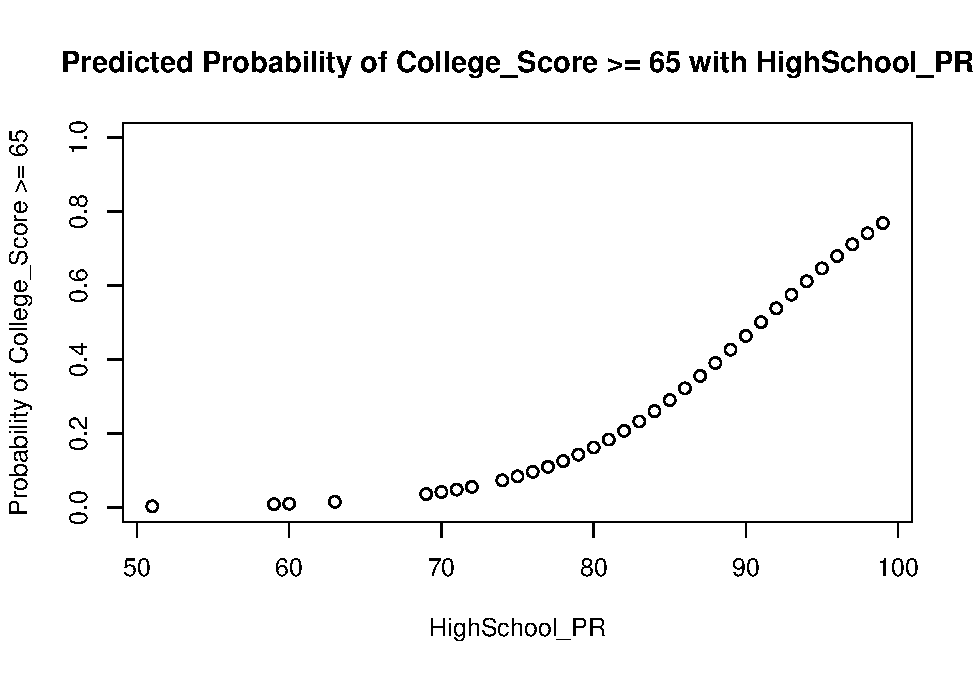
\includegraphics{PTT_Analysis_of_Test_Scores_Unfinished_files/figure-latex/validation-draft-1.pdf}

Since there are many repetitive values in \textbf{HighSchool\_PR}, let's
apply the \texttt{jitter} function to add random noise to the data for
display. (Remember to set a random seed for reproducibility.) We can see
that the deeper black circles indicate more records in the data, which
are concentrated in the higher \textbf{HighSchool\_PR} values.

\begin{Shaded}
\begin{Highlighting}[]
\CommentTok{\# Add jittering because of many repetitive values in HighSchool\_PR}
\FunctionTok{set.seed}\NormalTok{(}\DecValTok{21}\NormalTok{)}
\NormalTok{new\_xx }\OtherTok{=} \FunctionTok{jitter}\NormalTok{(xx)}
\NormalTok{new\_yy }\OtherTok{=} \FunctionTok{jitter}\NormalTok{(yy)}
\FunctionTok{plot}\NormalTok{(new\_xx, new\_yy, }\AttributeTok{ylim=}\FunctionTok{c}\NormalTok{(}\DecValTok{0}\NormalTok{,}\DecValTok{1}\NormalTok{),}
     \AttributeTok{main=}\StringTok{"Jittered Probability of College\_Score \textgreater{}= 65 with HighSchool\_PR"}\NormalTok{,}
     \AttributeTok{xlab=}\StringTok{"HighSchool\_PR"}\NormalTok{,}
     \AttributeTok{ylab=}\StringTok{"Probability of College\_Score \textgreater{}= 65"}\NormalTok{)}
\end{Highlighting}
\end{Shaded}

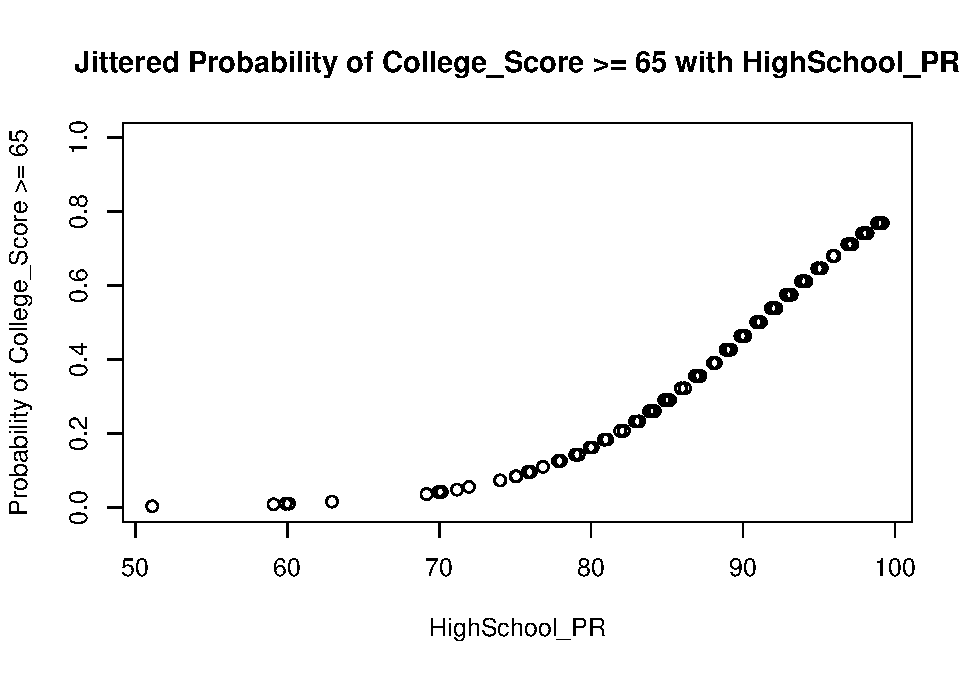
\includegraphics{PTT_Analysis_of_Test_Scores_Unfinished_files/figure-latex/validation-jittering-1.pdf}

\hypertarget{validation}{%
\section{Model Validation: In-Sample Prediction}\label{validation}}

We built the logistic regression model in Chapter \ref{logit-reg}, and
now it is time for model validation, i.e., evaluate the model
performance. We will focus on machine learning concepts in this chapter,
and the readers simply need to know that \textbf{the model does binary
classification}. For more about machine learning, we recommend the book
\emph{Introduction to Machine Learning}
\citep{alpaydin2020introduction}. It explains a wide range of machine
learning algorithms and applications, including the recent advances in
deep learning and neural networks.

We start with in-sample prediction to obtain the binary classification
results, then we explain how to interpret the 2x2 confusion matrix
output. There are two actual outcomes for \textbf{College\_Score} -- at
least 65 or not. There are also two predicted outcomes for
\textbf{College\_Score}, and we compare the predicted outcomes with the
actual ones. Next, we would like to examine the model performance for
different \textbf{HighSchool\_PR} scores, in order to identify whether
the model does better in higher or lower \textbf{HighSchool\_PR}, or
performs about the same. In Chapter \ref{out-of-sample}, we will perform
out-of-sample prediction on the model; that is, train the model on some
data and test it on different data.

\hypertarget{in-sample}{%
\subsection{Implementation of In-Sample Prediction}\label{in-sample}}

Let's start the model validation with in-sample prediction; that is,
using the data to predict the outcome of whether \textbf{College\_Score}
is at least 65 for each value of \textbf{HighSchool\_PR} for values
already in the data. If predicted probability of \textbf{College\_Score}
at least 65 (i.e., \texttt{fitted.values}) is greater than or equal to
0.5, we assign the predicted value as \texttt{TRUE}. We can safely use
0.5 as the probability threshold because the data are quite balanced. In
other words, the proportion of \textbf{College\_Score} at least 65 is
close to 0.5 in the data (0.489, to be exact). If the data are
imbalanced, say 80\% of the records belong to one category, we should
adjust the probability threshold in our classification prediction model.

\begin{Shaded}
\begin{Highlighting}[]
\CommentTok{\# nrow(data\_corr) \# 188}
\CommentTok{\# sum(data\_corr$CS\_65up) \# 92}
\CommentTok{\# sum(data\_corr$CS\_65up)/nrow(data\_corr) \# 0.489}

\FunctionTok{print}\NormalTok{(}\FunctionTok{paste}\NormalTok{(}\StringTok{"There are"}\NormalTok{,}\FunctionTok{nrow}\NormalTok{(data\_corr),}\StringTok{"records in the data, with"}\NormalTok{,}
            \FunctionTok{sum}\NormalTok{(data\_corr}\SpecialCharTok{$}\NormalTok{CS\_65up),}
            \StringTok{"of them have College\_Score at least 65."}\NormalTok{))}
\end{Highlighting}
\end{Shaded}

\begin{verbatim}
## [1] "There are 188 records in the data, with 92 of them have College_Score at least 65."
\end{verbatim}

\begin{Shaded}
\begin{Highlighting}[]
\FunctionTok{print}\NormalTok{(}\FunctionTok{paste}\NormalTok{(}\StringTok{"This is a proportion of"}\NormalTok{,}
            \FunctionTok{round}\NormalTok{(}\FunctionTok{sum}\NormalTok{(data\_corr}\SpecialCharTok{$}\NormalTok{CS\_65up)}\SpecialCharTok{/}\FunctionTok{nrow}\NormalTok{(data\_corr),}\AttributeTok{digits=}\DecValTok{3}\NormalTok{),}
            \StringTok{", which is close to 0.5."}\NormalTok{))}
\end{Highlighting}
\end{Shaded}

\begin{verbatim}
## [1] "This is a proportion of 0.489 , which is close to 0.5."
\end{verbatim}

Let's create a confusion matrix to show the comparison between the
actual outcomes and predicted outcomes, i.e., whether each respondent
obtained \textbf{College\_Score} at least 65 or not. Note that a
confusion matrix is slightly different than the contingency table in
Section \ref{examine-further}, although both record counts in a matrix.
A confusion matrix involves the predicted results, while a contingency
table simply observes the categories in the data.

\begin{Shaded}
\begin{Highlighting}[]
\CommentTok{\# Data}
\NormalTok{actual\_65up }\OtherTok{=}\NormalTok{ data\_corr}\SpecialCharTok{$}\NormalTok{CS\_65up}

\CommentTok{\# Predicted results}
\NormalTok{predicted\_65up }\OtherTok{=}\NormalTok{ model}\SpecialCharTok{$}\NormalTok{fitted.values }\SpecialCharTok{\textgreater{}=} \FloatTok{0.5}

\CommentTok{\# Confusion matrix}
\NormalTok{confusion }\OtherTok{=} \FunctionTok{table}\NormalTok{(actual\_65up, predicted\_65up)}
\CommentTok{\# revert the order of FALSE and TRUE}
\NormalTok{confusion }\OtherTok{=}\NormalTok{ confusion[}\DecValTok{2}\SpecialCharTok{:}\DecValTok{1}\NormalTok{, }\DecValTok{2}\SpecialCharTok{:}\DecValTok{1}\NormalTok{] }
\NormalTok{confusion}
\end{Highlighting}
\end{Shaded}

\begin{verbatim}
##            predicted_65up
## actual_65up TRUE FALSE
##       TRUE    72    20
##       FALSE   35    61
\end{verbatim}

Below is the percentage version of the confusion matrix.

\begin{Shaded}
\begin{Highlighting}[]
\FunctionTok{prop.table}\NormalTok{(confusion)}
\end{Highlighting}
\end{Shaded}

\begin{verbatim}
##            predicted_65up
## actual_65up      TRUE     FALSE
##       TRUE  0.3829787 0.1063830
##       FALSE 0.1861702 0.3244681
\end{verbatim}

The table below shows the meaning of each cell of the confusion matrix.
Assume that ``positive'' means getting \textbf{College\_Score} at least
65, which is equivalent to the \texttt{TRUE} label in
\texttt{actual\_65up} and \texttt{predicted\_65up}. The term
``negative'' means not getting \textbf{College\_Score} at least 65, so
it is equivalent to the \texttt{FALSE} label. For each cell, we
have:\footnote{\url{https://developers.google.com/machine-learning/crash-course/classification/true-false-positive-negative}}

\begin{itemize}
\tightlist
\item
  \textbf{True Positive (TP)}: The datapoint is actually positive and is
  predicted as positive, so the model correctly predicts the positive
  outcome.
\item
  \textbf{True Negative (TN)}: The datapoint is actually negative and is
  predicted as negative, so the model correctly predicts the negative
  outcome.
\item
  \textbf{False Positive (FP)}: The datapoint is actually negative but
  is predicted as positive, so the model \textbf{in}correctly predicts
  the positive outcome, i.e., false alarm.
\item
  \textbf{False Negative (FN)}: The datapoint is actually positive but
  is predicted as negative, so the model \textbf{in}correctly predicts
  the negative outcome, i.e., error.
\end{itemize}

\begin{verbatim}
##                 | Predicted Positive | Predicted Negative
## --------------  | ------------------ | ------------------
## Actual Positive |      True Positive |     False Negative
## --------------- | ------------------ | ------------------
## Actual Negative |     False Positive |      True Negative
\end{verbatim}

We can retrieve each element in the confusion matrix by specifying the
labels for each row and each column. The row indicates how many
respondents actually obtained \textbf{College\_Score} at least 65, and
the column indicates how many respondents were predicted to have the
positive outcome. Instead of writing the syntax like
\texttt{confusion{[}1,2{]}}, we write it in a clearer way
\texttt{confusion{[}"TRUE","FALSE"{]}}. (Don't make the confusion matrix
more confusing!) The readers can easily see that this is the number of
respondents who we did not predict to have a \textbf{College\_Score} at
least 65, but they actually did.

\begin{Shaded}
\begin{Highlighting}[]
\CommentTok{\# row = actual\_65up, column = predicted\_65up}
\NormalTok{tp }\OtherTok{=}\NormalTok{ confusion[}\StringTok{"TRUE"}\NormalTok{,}\StringTok{"TRUE"}\NormalTok{]}
\NormalTok{fn }\OtherTok{=}\NormalTok{ confusion[}\StringTok{"TRUE"}\NormalTok{,}\StringTok{"FALSE"}\NormalTok{]}
\NormalTok{fp }\OtherTok{=}\NormalTok{ confusion[}\StringTok{"FALSE"}\NormalTok{,}\StringTok{"TRUE"}\NormalTok{]}
\NormalTok{tn }\OtherTok{=}\NormalTok{ confusion[}\StringTok{"FALSE"}\NormalTok{,}\StringTok{"FALSE"}\NormalTok{]}

\FunctionTok{print}\NormalTok{(}\FunctionTok{paste}\NormalTok{(tp,fn,fp,tn))}
\end{Highlighting}
\end{Shaded}

\begin{verbatim}
## [1] "72 20 35 61"
\end{verbatim}

We can also verify that the retrieved numbers are exactly the same as in
the original confusion matrix.

\begin{Shaded}
\begin{Highlighting}[]
\NormalTok{confusion}
\end{Highlighting}
\end{Shaded}

\begin{verbatim}
##            predicted_65up
## actual_65up TRUE FALSE
##       TRUE    72    20
##       FALSE   35    61
\end{verbatim}

\hypertarget{interpretation}{%
\subsection{Interpretation of Confusion Matrix}\label{interpretation}}

After creating the confusion matrix to record the model performance, we
need to interpret the numbers and define metrics to measure the
performance. We start with the overall \textbf{accuracy} to calculate
how many datapoints the model predicted correctly. A datapoint is
correctly predicted if one of the two scenarios occurs:

\begin{itemize}
\tightlist
\item
  True Positive: The datapoint is actually positive and it is predicted
  as positive.
\item
  True Negative: The datapoint is actually negative and it is predicted
  as negative.
\end{itemize}

In the context of our dataset, ``positive'' means getting a
\textbf{College\_Score} 65 or higher, and ``negative'' means getting a
\textbf{College\_Score} of 64 or lower. We run the model to predict the
respondents' college entrance exam outcome given their
\textbf{HighSchool\_PR}. In mathematical terms, accuracy can be
calculated as below:

\[\text{Accuracy} = \dfrac{\text{True Positive + True Negative}}{\text{Actual Positive + Actual Negative}} = \dfrac{\text{True Positive + True Negative}}{\text{All Datapoints}}\]

Plugging in the numbers from our model, we get
\[\text{Accuracy} = \dfrac{72+61}{72+20+35+61} \approx 70.74\%.\] Our
model correctly predicts whether the \textbf{College\_Score} would be at
least 65 or not around 70\% of the time, which is better than a 50-50
coin flip. This means our model is informative, and the results align
with the prior knowledge that a higher \textbf{HighSchool\_PR} is more
likely to lead to \textbf{College\_Score} at least 65.

Note that when the data are imbalanced (say, 98\% of the records belong
to one category), accuracy is not a good measure of model
performance.\footnote{\url{https://www.analyticsvidhya.com/blog/2017/03/imbalanced-data-classification/}}
The model can simply predict all datapoints to be in the larger
category, and achieve 98\% accuracy. The good news is that we get a
relatively balanced dataset by setting the classification threshold of
\textbf{College\_Score} to be 65, as we explained at the beginning of
Section \ref{threshold-65}. In fact, 48.9\% of the respondents have a
\textbf{College\_Score} of 65 or higher.

\begin{Shaded}
\begin{Highlighting}[]
\FunctionTok{print}\NormalTok{(}\FunctionTok{paste}\NormalTok{(}\StringTok{"The proportion of respondents with College\_Score 65 or higher is"}\NormalTok{,}
            \FunctionTok{round}\NormalTok{(}\FunctionTok{sum}\NormalTok{(data\_corr}\SpecialCharTok{$}\NormalTok{CS\_65up)}\SpecialCharTok{/}\FunctionTok{nrow}\NormalTok{(data\_corr), }\AttributeTok{digits =} \DecValTok{3}\NormalTok{)))}
\end{Highlighting}
\end{Shaded}

\begin{verbatim}
## [1] "The proportion of respondents with College_Score 65 or higher is 0.489"
\end{verbatim}

\subsubsection{Precision and Recall}

\textbf{Precision} and \textbf{recall} are also two widely-used metrics
to measure the performance of the prediction model, and most
importantly, they do not depend much on the proportions of data
categories. Precision is defined as the percentage of true positives
among all datapoints the model predicted to be positive. In our example,
precision is the percentage of the respondents who actually got
\textbf{College\_Score} at least 65, among the respondents we predicted
to make this achievement given their \textbf{HighSchool\_PR}.

\[\text{Precision} = \dfrac{\text{True Positive}}{\text{Predicted Positive}} = \dfrac{\text{True Positive}}{\text{True Positive + False Positive}}\]

Plugging in the numbers from our model, we get
\[\text{Precision} = \dfrac{72}{72+35} \approx 67.29\%.\]

The precision would be useful if we use the predictive information to
decide to invest in which high school students based on their
\textbf{HighSchool\_PR}. If we predict a student to get
\textbf{College\_Score} at least 65, he/she has about a 67.29\% chance
to make it, which is more than two-thirds. Since there are different
tiers of high schools in Taiwan based on \textbf{HighSchool\_PR}, many
resources are given to the top tier high schools, because these students
have the highest chance to do well on the college entrance exam.
Nevertheless, other social factors also play a role in the overall
policy decision-making process. For example, the government may decide
to put more resources into remote rural high schools to empower
disadvantaged students to succeed, which is beneficial for upward social
mobility.

On the other hand, recall is defined as the percentage of
model-predicted positives among all datapoints that are actually
positive. In our example, recall is the percentage of the respondents we
predicted to have \textbf{College\_Score} at least 65 given their
\textbf{HighSchool\_PR}, among the respondents who actually made this
achievement.

\[\text{Recall} = \dfrac{\text{True Positive}}{\text{Actual Positive}} = \dfrac{\text{True Positive}}{\text{True Positive + False Negative}}\]

Plugging in the numbers from our model, we get
\[\text{Recall} = \dfrac{72}{72+20} \approx 78.26\%.\]

The recall would also be useful if we use the predictive information to
decide to invest in which high school students based on their
\textbf{HighSchool\_PR}. We need to remember that among the high school
graduates who got a \textbf{College\_Score} at least 65, only 78.26\% of
them were predicted to have such potential. In other words, the
remaining 21.74\% of high school students did better than the predictive
model had expected. It is possible that they were smart but accidentally
did poorly on the high school entrance exam, and they would have
achieved \textbf{College\_Score} at least 65 regardless. Another
possibility is that they did not study much in middle school and got a
low \textbf{HighSchool\_PR}, but they received extra help and/or studied
much harder for the college entrance exam to get a
\textbf{College\_Score} at least 65. The lesson is that by pre-selecting
students based on \textbf{HighSchool\_PR}, we would still get some
``dark horses'', i.e., the students who performed much better on the
\textbf{College\_Score} than we had expected.

\subsubsection{False Positive Rate and False Negative Rate}

\textbf{False positive rate} and \textbf{false negative rate} are
typically used to measure the accuracy of a medical screening test for a
disease \citep{diagnosis-test}, where ``positive'' means having the
disease and ``negative'' means not having the disease. In our dataset,
``positive'' means something much better -- getting a
\textbf{College\_Score} 65 or higher. ``Negative'' means not achieving
this.

False positive rate is the probability of an actual negative being
classified as a positive, and it is also called a ``false alarm''. In
medical terms, this means someone is tested positive for a disease, but
actually does not have it. In our dataset, this means a student was
predicted to get \textbf{College\_Score} at least 65, but actually did
not.

\[\text{False Positive Rate} = \dfrac{\text{False Positive}}{\text{Actual Negative}} = \dfrac{\text{False Positive}}{\text{True Negative + False Positive}}\]

Plugging in the numbers from our model, we get
\[\text{False Positive Rate} = \dfrac{35}{35+61} \approx 36.46\%.\]

Given that a student did not get \textbf{College\_Score} at least 65,
there is a 36.46\% chance that we predicted him/her to achieve this. We
would like to give the benefit of the doubt, saying that the student
simply did not do well on the first college entrance exam for early
admission. It is possible that he/she was able to get into a better
school through taking the second college entrance exam for regular
admission.

On the other hand, false negative rate is the probability of an actual
positive being classified as a negative. In medical terms, this means
someone is tested negative for a disease, but actually has the disease.
In our dataset, this means a student actually got
\textbf{College\_Score} at least 65, but we predicted him/her as not
achieving this.

\[\text{False Negative Rate} = \dfrac{\text{False Negative}}{\text{Actual Positive}} = \dfrac{\text{False Negative}}{\text{True Positive + False Negative}}\]

False negative rate means how likely the model missed actual positive
datapoints, so this rate is the opposite of recall.

\[\text{False Negative Rate} = 1 - \text{Recall}\]

Plugging in the numbers from our model, we get
\[\text{False Negative Rate} = \dfrac{20}{72+20} \approx 21.74\%.\]

Given that a student actually got \textbf{College\_Score} at least 65,
there is a 21.74\% chance that we did not predict him/her to achieve
this. We need to remember that the model is imperfect, so there always
exist students who did better in \textbf{College\_Score} than the model
had expected. To put it differently, \textbf{HighSchool\_PR} is not a
full indicator of achieving \textbf{College\_Score} at least 65 or not.
This is an encouraging message to students who did not do well in
\textbf{HighSchool\_PR}, because they still have a chance in
\textbf{College\_Score} to get admitted to a good school.

In our data analysis, false positive rate and false negative rate have
about equal importance. But in certain situations, one can be much more
important than the other. For instance, false positive rate is an
essential measure in the effectiveness of prompting users to re-enter
login information to verify identity for social media. The goal of
re-entering credentials is to prevent unauthorized logins, but when
people get prompted too many times while using their own account, they
would get frustrated and leave the website. This leads to significant
revenue loss in business.\footnote{\url{https://fcase.io/a-major-challenge-false-positives/}}
On the contrary, we are more concerned about the false negative rate in
medical testing for a rare disease. The goal of medical testing is to
identify as many people with the disease as possible, so that these
people can receive timely medical treatment. Hence we are more concerned
when the test fails to detect a person who actually has the
disease.\footnote{\url{https://brownmath.com/stat/falsepos.htm}}

\subsubsection{Sensitivity and Specificity}

We are going off on a tangent here, because this section is not directly
related to the data of high school and college entrance exam scores. But
we think it is important to introduce the concepts of
\textbf{sensitivity} and \textbf{specificity} to the readers, since they
are also used to describe the overall testing results, especially in a
clinical setting.\footnote{\url{https://www.healthnewsreview.org/toolkit/tips-for-understanding-studies/understanding-medical-tests-sensitivity-specificity-and-positive-predictive-value/}}

Sensitivity means that when a patient actually has the disease (actual
positive), the medical test is able to sense it and produce a positive
result. That is, the medical test is sensitive enough to identify
patients who have the disease.

\[\text{Sensitivity} = \dfrac{\text{True Positive}}{\text{Actual Positive}} = \dfrac{\text{True Positive}}{\text{True Positive + False Negative}}.\]
Sensitivity is equivalent to the true positive rate (a.k.a. recall), or
the opposite of the false negative rate.

\[\text{Sensitivity} = \text{Recall} = 1 - \text{False Negative Rate}.\]

On the other hand, specificity means when a patient does not have the
disease (actual negative), the medical test is able to produce a
negative result. That is, the medical test is specific enough that it
filters out patients who do not have the disease.

\[\text{Specificity} = \dfrac{\text{True Negative}}{\text{Actual Negative}} = \dfrac{\text{True Negative}}{\text{True Negative + False Positive}}.\]
Specificity is equivalent to the true negative rate, or the opposite of
the false positive rate.

\[\text{Specificity} = 1 - \text{False Positive Rate}.\]

Let's see an example in medical testing.\footnote{\url{https://math.hmc.edu/funfacts/medical-tests-and-bayes-theorem/}}
Assume 0.1\% of the population have a specific disease. In a population
of 500,000 people, 500 people would have the disease. Now we have a
medical test that claims to be 99\% accurate, which means the test has
99\% sensitivity and 99\% specificity. Hence the false positive rate and
the false negative rate are both 1\%.

\begin{itemize}
\item
  For the 500 people who actually have the disease, 495 tested positive
  and 5 tested negative.
\item
  For the 499,500 people who do not have the disease, 4,995 people
  tested positive and the remaining 494,505 people tested negative.
\end{itemize}

\textbf{Given that a patient tested positive, how likely does he/she
actually have the disease?}

Using the Bayes theorem, we get

\[\begin{aligned}
& P(\text{Actual Positive}|\text{Test Positive}) = \dfrac{P(\text{Actual Positive} \cap \text{Test Positive})}{P(\text{Test Positive})}\\
&= \dfrac{P(\text{Actual Positive} \cap \text{Test Positive})}{P(\text{Actual Positive} \cap \text{Test Positive}) + P(\text{Actual Negative} \cap \text{Test Positive})}\\
&= \dfrac{495}{495 + 4995} \approx 9.16\%.
\end{aligned}\]

\textbf{The patient has a 9.16\% of chance of actually having the
disease, despite the positive test outcome. The patient does not have
the disease for more than 90\% of the time.} Since the disease infects
only 0.1\% of the population, the medical test creates many false
positives, i.e., false alarms. Nevertheless, the test is still
informative because given a positive test result, the probability of the
patient having the disease increases by 91.6 times.

\[\dfrac{P(\text{Actual Positive}|\text{Test Positive})}{P(\text{Actual Positive})} = \dfrac{9.16\%}{0.1\%} = 91.6.\]

The statistical calculation tells us that we do not have to be overly
concerned about a positive medical test outcome, because the chances are
still low for the person to have the disease. However, upon learning the
99\% sensitivity and 99\% specificity of the test, many doctors seem to
associate a positive test with a high probability of having the
disease.\footnote{\url{https://www.washingtonpost.com/news/posteverything/wp/2018/10/05/feature/doctors-are-surprisingly-bad-at-reading-lab-results-its-putting-us-all-at-risk/}}
If any of the readers become a medical doctor in the future, please
remember the lesson here and make better treatment decisions for the
patients.

\hypertarget{another-breakdown}{%
\subsection{Breakdown by High School Entrance Exam
Scores}\label{another-breakdown}}

\section*{\textcolor{red}{Unfinished below}}

Add my thoughts about categorical data analysis (e.g.~proportional
hazards model?!)

Example: When \textbf{HighSchool\_PR} is increased from Category X to
Category Y, how does it affect the categories of
\textbf{College\_Score}?

You don't have to do the full implementation, just write a few lines as
a pointer to the concepts.

\textcolor{red}{This is the file we want to move content into.}

\section*{\textcolor{red}{Unfinished above}}

Let's examine the confusion matrices for each group of
\textbf{HighSchool\_PR}: 0-79, 80-89, 90-94, 95-99. We would like to see
if the model performance varies across these groups. Readers can refer
to Section \ref{HighSchool-PR-80-up} for the details of this
categorization. Before going into the analysis, we need to ensure that
each group has a sufficiently large number of respondents within the 188
total records.

The group with \textbf{HighSchool\_PR} 0-79 has the smallest number of
respondents, and 25 is a sufficient sample size. The groups with
\textbf{HighSchool\_PR} 80-89 and 90-94 contain 49 and 44 respondents,
respectively. The group with \textbf{HighSchool\_PR} 95-99 includes 70
respondents, which is the largest of the four categories.

\begin{Shaded}
\begin{Highlighting}[]
\NormalTok{HS0to79\_ind }\OtherTok{=} \FunctionTok{which}\NormalTok{(data\_corr}\SpecialCharTok{$}\NormalTok{HighSchool\_PR }\SpecialCharTok{\textgreater{}=}\DecValTok{0} \SpecialCharTok{\&}\NormalTok{ data\_corr}\SpecialCharTok{$}\NormalTok{HighSchool\_PR }\SpecialCharTok{\textless{}=} \DecValTok{79}\NormalTok{)}
\NormalTok{HS80to89\_ind }\OtherTok{=} \FunctionTok{which}\NormalTok{(data\_corr}\SpecialCharTok{$}\NormalTok{HighSchool\_PR }\SpecialCharTok{\textgreater{}=} \DecValTok{80} \SpecialCharTok{\&}\NormalTok{ data\_corr}\SpecialCharTok{$}\NormalTok{HighSchool\_PR }\SpecialCharTok{\textless{}=} \DecValTok{89}\NormalTok{)}
\NormalTok{HS90to94\_ind }\OtherTok{=} \FunctionTok{which}\NormalTok{(data\_corr}\SpecialCharTok{$}\NormalTok{HighSchool\_PR }\SpecialCharTok{\textgreater{}=} \DecValTok{90} \SpecialCharTok{\&}\NormalTok{ data\_corr}\SpecialCharTok{$}\NormalTok{HighSchool\_PR }\SpecialCharTok{\textless{}=} \DecValTok{94}\NormalTok{)}
\NormalTok{HS95to99\_ind }\OtherTok{=} \FunctionTok{which}\NormalTok{(data\_corr}\SpecialCharTok{$}\NormalTok{HighSchool\_PR }\SpecialCharTok{\textgreater{}=} \DecValTok{95} \SpecialCharTok{\&}\NormalTok{ data\_corr}\SpecialCharTok{$}\NormalTok{HighSchool\_PR }\SpecialCharTok{\textless{}=} \DecValTok{99}\NormalTok{)}

\FunctionTok{print}\NormalTok{(}\FunctionTok{paste}\NormalTok{(}\StringTok{"HighSchool\_PR 0{-}79:"}\NormalTok{,}\FunctionTok{length}\NormalTok{(HS0to79\_ind), }\StringTok{"respondents"}\NormalTok{))}
\end{Highlighting}
\end{Shaded}

\begin{verbatim}
## [1] "HighSchool_PR 0-79: 25 respondents"
\end{verbatim}

\begin{Shaded}
\begin{Highlighting}[]
\FunctionTok{print}\NormalTok{(}\FunctionTok{paste}\NormalTok{(}\StringTok{"HighSchool\_PR 80{-}89:"}\NormalTok{,}\FunctionTok{length}\NormalTok{(HS80to89\_ind), }\StringTok{"respondents"}\NormalTok{))}
\end{Highlighting}
\end{Shaded}

\begin{verbatim}
## [1] "HighSchool_PR 80-89: 49 respondents"
\end{verbatim}

\begin{Shaded}
\begin{Highlighting}[]
\FunctionTok{print}\NormalTok{(}\FunctionTok{paste}\NormalTok{(}\StringTok{"HighSchool\_PR 90{-}94:"}\NormalTok{,}\FunctionTok{length}\NormalTok{(HS90to94\_ind), }\StringTok{"respondents"}\NormalTok{))}
\end{Highlighting}
\end{Shaded}

\begin{verbatim}
## [1] "HighSchool_PR 90-94: 44 respondents"
\end{verbatim}

\begin{Shaded}
\begin{Highlighting}[]
\FunctionTok{print}\NormalTok{(}\FunctionTok{paste}\NormalTok{(}\StringTok{"HighSchool\_PR 95{-}99:"}\NormalTok{,}\FunctionTok{length}\NormalTok{(HS95to99\_ind), }\StringTok{"respondents"}\NormalTok{))}
\end{Highlighting}
\end{Shaded}

\begin{verbatim}
## [1] "HighSchool_PR 95-99: 70 respondents"
\end{verbatim}

Now we can produce a confusion matrix for each of the four groups.
Except for \textbf{HighSchool\_PR} 90-94, all the other three groups
contain only one value in the predicted outcomes. The higher
\textbf{HighSchool\_PR} the student had, the higher probability the
model would predict him/her to achieve \textbf{College\_Score} at least
65. This is not completely unexpected, but we would like to emphasize
that the model is imperfect. There are still some students with a low
\textbf{HighSchool\_PR} but an impressively good
\textbf{College\_Score}.

\begin{itemize}
\tightlist
\item
  \textbf{HighSchool\_PR} 0-79 has only FALSE predicted outcomes in
  \textbf{College\_Score} at least 65.
\item
  \textbf{HighSchool\_PR} 80-89 has only FALSE predicted outcomes in
  \textbf{College\_Score} at least 65.
\item
  \textbf{HighSchool\_PR} 90-94 has TRUE and FALSE predicted outcomes in
  \textbf{College\_Score} at least 65.
\item
  \textbf{HighSchool\_PR} 95-99 has only TRUE predicted outcomes in
  \textbf{College\_Score} at least 65.
\end{itemize}

When the predicted outcomes do not include both TRUE and FALSE, the
confusion matrix produced in \texttt{R} would be 2x1 instead of the full
2x2. Section \ref{confusion-2x1} shows the incorrect 2x1 confusion
matrices, and we will add the missing second column back in Section
\ref{confusion-2x2-full}. Finally, we will interpret these results in
Section \ref{segment-interpret}.

\hypertarget{confusion-2x1}{%
\subsubsection{Confusion Matrices (Incorrect)}\label{confusion-2x1}}

Let's write a function to summarize the actual outcomes and the
predicted outcomes into a confusion matrix, using the default settings
in \texttt{table}. As the readers can see, \texttt{table} outputs only
the nonzero columns, and that's why we have several 2x1 confusion
matrices here.

\begin{Shaded}
\begin{Highlighting}[]
\CommentTok{\# Data}
\NormalTok{actual\_65up }\OtherTok{=}\NormalTok{ data\_corr}\SpecialCharTok{$}\NormalTok{CS\_65up}
\CommentTok{\# Predicted results}
\NormalTok{predicted\_65up }\OtherTok{=}\NormalTok{ model}\SpecialCharTok{$}\NormalTok{fitted.values }\SpecialCharTok{\textgreater{}=} \FloatTok{0.5}

\NormalTok{confusion\_original }\OtherTok{\textless{}{-}} \ControlFlowTok{function}\NormalTok{(HS\_inds, actual, predicted) \{}
\NormalTok{  actual }\OtherTok{=}\NormalTok{ actual[HS\_inds]}
\NormalTok{  predicted }\OtherTok{=}\NormalTok{ predicted[HS\_inds]}
\NormalTok{  confusion }\OtherTok{=} \FunctionTok{table}\NormalTok{(actual, predicted)}
  \FunctionTok{return}\NormalTok{(confusion)}
\NormalTok{\}}
\end{Highlighting}
\end{Shaded}

Confusion matrix for \textbf{HighSchool\_PR} 0-79

\begin{Shaded}
\begin{Highlighting}[]
\NormalTok{confusion\_0to79 }\OtherTok{=} \FunctionTok{confusion\_original}\NormalTok{(HS0to79\_ind, actual\_65up, predicted\_65up)}
\NormalTok{confusion\_0to79}
\end{Highlighting}
\end{Shaded}

\begin{verbatim}
##        predicted
## actual  FALSE
##   FALSE    21
##   TRUE      4
\end{verbatim}

Confusion matrix for \textbf{HighSchool\_PR} 80-89

\begin{Shaded}
\begin{Highlighting}[]
\NormalTok{confusion\_80to89 }\OtherTok{=} \FunctionTok{confusion\_original}\NormalTok{(HS80to89\_ind, actual\_65up, predicted\_65up)}
\NormalTok{confusion\_80to89}
\end{Highlighting}
\end{Shaded}

\begin{verbatim}
##        predicted
## actual  FALSE
##   FALSE    35
##   TRUE     14
\end{verbatim}

Confusion matrix for \textbf{HighSchool\_PR} 90-94

\begin{Shaded}
\begin{Highlighting}[]
\NormalTok{confusion\_90to94 }\OtherTok{=} \FunctionTok{confusion\_original}\NormalTok{(HS90to94\_ind, actual\_65up, predicted\_65up)}
\NormalTok{confusion\_90to94}
\end{Highlighting}
\end{Shaded}

\begin{verbatim}
##        predicted
## actual  FALSE TRUE
##   FALSE     5   22
##   TRUE      2   15
\end{verbatim}

Confusion matrix for \textbf{HighSchool\_PR} 95-99

\begin{Shaded}
\begin{Highlighting}[]
\NormalTok{confusion\_95to99 }\OtherTok{=} \FunctionTok{confusion\_original}\NormalTok{(HS95to99\_ind, actual\_65up, predicted\_65up)}
\NormalTok{confusion\_95to99}
\end{Highlighting}
\end{Shaded}

\begin{verbatim}
##        predicted
## actual  TRUE
##   FALSE   13
##   TRUE    57
\end{verbatim}

\hypertarget{confusion-2x2-full}{%
\subsubsection{Confusion Matrices (Correct)}\label{confusion-2x2-full}}

When the confusion matrix has nonzero values in all four cells, we can
output the 2x2 confusion matrix. But before doing so, we need to revert
the order of FALSE and TRUE in the rows and columns, since \texttt{R}
sorts names in alphabetical order by default. This can be done by
producing the second index (TRUE) before the first index (FALSE).

When all predicted values are FALSE, the confusion matrix is missing a
TRUE column and we need to add it back. Similarly, When all predicted
values are TRUE, the confusion matrix is missing a FALSE column and we
also need to add it back. Finally, we revert the order of FALSE and TRUE
in the rows and columns, as in the case of an 2x2 confusion matrix.

By checking the dimensions of the confusing matrices and modifying if
necessary, we obtain all four 2x2 confusion matrices for the four
categories of \textbf{HighSchool\_PR}.

\begin{Shaded}
\begin{Highlighting}[]
\NormalTok{confusion\_subset }\OtherTok{\textless{}{-}} \ControlFlowTok{function}\NormalTok{(HS\_inds, actual, predicted) \{}
\NormalTok{  actual }\OtherTok{=}\NormalTok{ actual[HS\_inds]}
\NormalTok{  predicted }\OtherTok{=}\NormalTok{ predicted[HS\_inds]}
\NormalTok{  confusion }\OtherTok{=} \FunctionTok{table}\NormalTok{(actual, predicted)}
  
  \CommentTok{\# When the confusion matrix has nonzero values in all four cells}
  \ControlFlowTok{if}\NormalTok{ ((}\FunctionTok{dim}\NormalTok{(confusion)[}\DecValTok{1}\NormalTok{] }\SpecialCharTok{==} \DecValTok{2}\NormalTok{) }\SpecialCharTok{\&\&}\NormalTok{ (}\FunctionTok{dim}\NormalTok{(confusion)[}\DecValTok{2}\NormalTok{] }\SpecialCharTok{==} \DecValTok{2}\NormalTok{)) \{}
    \CommentTok{\# Revert the order of FALSE and TRUE}
\NormalTok{    confusion }\OtherTok{=}\NormalTok{ confusion[}\DecValTok{2}\SpecialCharTok{:}\DecValTok{1}\NormalTok{, }\DecValTok{2}\SpecialCharTok{:}\DecValTok{1}\NormalTok{]}
    \CommentTok{\# Exit the function because the operation is complete}
    \FunctionTok{return}\NormalTok{(confusion)}
\NormalTok{  \}}
  
  \CommentTok{\# When all predicted values are FALSE}
  \ControlFlowTok{else} \ControlFlowTok{if}\NormalTok{ (}\FunctionTok{colnames}\NormalTok{(confusion) }\SpecialCharTok{==} \FunctionTok{c}\NormalTok{(}\StringTok{"FALSE"}\NormalTok{)) \{}
\NormalTok{    confusion }\OtherTok{=} \FunctionTok{as.table}\NormalTok{(}\FunctionTok{cbind}\NormalTok{(confusion,}\FunctionTok{c}\NormalTok{(}\DecValTok{0}\NormalTok{,}\DecValTok{0}\NormalTok{)))}
    \FunctionTok{colnames}\NormalTok{(confusion) }\OtherTok{=} \FunctionTok{c}\NormalTok{(}\StringTok{"FALSE"}\NormalTok{,}\StringTok{"TRUE"}\NormalTok{)}
    \FunctionTok{names}\NormalTok{(}\FunctionTok{dimnames}\NormalTok{(confusion)) }\OtherTok{=} \FunctionTok{c}\NormalTok{(}\StringTok{"actual"}\NormalTok{,}\StringTok{"predicted"}\NormalTok{)}
\NormalTok{  \}}
  
  \CommentTok{\# When all predicted values are TRUE}
  \ControlFlowTok{else} \ControlFlowTok{if}\NormalTok{ (}\FunctionTok{colnames}\NormalTok{(confusion) }\SpecialCharTok{==} \FunctionTok{c}\NormalTok{(}\StringTok{"TRUE"}\NormalTok{)) \{}
\NormalTok{    confusion }\OtherTok{=} \FunctionTok{as.table}\NormalTok{(}\FunctionTok{cbind}\NormalTok{(}\FunctionTok{c}\NormalTok{(}\DecValTok{0}\NormalTok{,}\DecValTok{0}\NormalTok{), confusion))}
    \FunctionTok{colnames}\NormalTok{(confusion) }\OtherTok{=} \FunctionTok{c}\NormalTok{(}\StringTok{"FALSE"}\NormalTok{,}\StringTok{"TRUE"}\NormalTok{)}
    \FunctionTok{names}\NormalTok{(}\FunctionTok{dimnames}\NormalTok{(confusion)) }\OtherTok{=} \FunctionTok{c}\NormalTok{(}\StringTok{"actual"}\NormalTok{,}\StringTok{"predicted"}\NormalTok{)}
\NormalTok{  \}}
  
  \CommentTok{\# Revert the order of FALSE and TRUE}
\NormalTok{  confusion }\OtherTok{=}\NormalTok{ confusion[}\DecValTok{2}\SpecialCharTok{:}\DecValTok{1}\NormalTok{, }\DecValTok{2}\SpecialCharTok{:}\DecValTok{1}\NormalTok{] }
  \FunctionTok{return}\NormalTok{(confusion)}
\NormalTok{\}}
\end{Highlighting}
\end{Shaded}

Confusion matrix for \textbf{HighSchool\_PR} 0-79

\begin{Shaded}
\begin{Highlighting}[]
\NormalTok{confusion\_0to79 }\OtherTok{=} \FunctionTok{confusion\_subset}\NormalTok{(HS0to79\_ind, actual\_65up, predicted\_65up)}
\NormalTok{confusion\_0to79}
\end{Highlighting}
\end{Shaded}

\begin{verbatim}
##        predicted
## actual  TRUE FALSE
##   TRUE     0     4
##   FALSE    0    21
\end{verbatim}

Confusion matrix for \textbf{HighSchool\_PR} 80-89

\begin{Shaded}
\begin{Highlighting}[]
\NormalTok{confusion\_80to89 }\OtherTok{=} \FunctionTok{confusion\_subset}\NormalTok{(HS80to89\_ind, actual\_65up, predicted\_65up)}
\NormalTok{confusion\_80to89}
\end{Highlighting}
\end{Shaded}

\begin{verbatim}
##        predicted
## actual  TRUE FALSE
##   TRUE     0    14
##   FALSE    0    35
\end{verbatim}

Confusion matrix for \textbf{HighSchool\_PR} 90-94

\begin{Shaded}
\begin{Highlighting}[]
\NormalTok{confusion\_90to94 }\OtherTok{=} \FunctionTok{confusion\_subset}\NormalTok{(HS90to94\_ind, actual\_65up, predicted\_65up)}
\NormalTok{confusion\_90to94}
\end{Highlighting}
\end{Shaded}

\begin{verbatim}
##        predicted
## actual  TRUE FALSE
##   TRUE    15     2
##   FALSE   22     5
\end{verbatim}

Confusion matrix for \textbf{HighSchool\_PR} 95-99

\begin{Shaded}
\begin{Highlighting}[]
\NormalTok{confusion\_95to99 }\OtherTok{=} \FunctionTok{confusion\_subset}\NormalTok{(HS95to99\_ind, actual\_65up, predicted\_65up)}
\NormalTok{confusion\_95to99}
\end{Highlighting}
\end{Shaded}

\begin{verbatim}
##        predicted
## actual  TRUE FALSE
##   TRUE    57     0
##   FALSE   13     0
\end{verbatim}

\hypertarget{segment-interpret}{%
\subsubsection{Interpretations}\label{segment-interpret}}

Table \ref{tab:breakdown-pr} shows the model results for each
\textbf{HighSchool\_PR} category (0-79, 80-89, 90-94, 95-99) -- in terms
of accuracy, precision, recall, FPR, and FNR. Any metric that cannot be
calculated is marked as N/A. The results are quite extreme because the
model predicted negative for all \textbf{HighSchool\_PR} 0-79 and 80-89,
and it predicted positive for all \textbf{HighSchool\_PR} 95-99. Here,
positive means achieving \textbf{College\_Score} 65 or higher, and
negative means not achieving this.

The overall accuracy is slightly above 70\%, while the accuracy for
\textbf{HighSchool\_PR} 90-94 is below 50\%. Nevertheless, the group of
\textbf{HighSchool\_PR} 90-94 is the only category with nonzero values
in all four cells of the confusion matrix. All the other three
\textbf{HighSchool\_PR} categories have good accuracy, but their FPR and
FNR are either 0\% or 100\% because all predictions within each group
have the same value.

\begin{table}[ht]
    \centering
    \begin{tabular}{|c|c|c|c|c|c|}
    \hline
    \textbf{HighSchool$\_$PR}   & Accuracy & Precision & Recall  & FPR     & FNR     \\ \hline
     0-79   & 84.00\% & N/A     & 0\%     & 0\%     & 100\% \\ \hline
    80-89   & 71.43\% & N/A     & 0\%     & 0\%     & 100\% \\ \hline
    90-94   & 45.45\% & 40.54\% & 88.23\% & 81.48\% & 11.76\% \\ \hline
    95-99   & 81.43\% & 81.43\% & 100\%   & 100\%   & 0\%     \\ \hline
    Overall & 70.74\% & 67.29\% & 78.26\% & 36.46\% & 21.74\% \\ \hline
    \end{tabular}
    \caption{Model results for each \textbf{HighSchool$\_$PR} category}
    \label{tab:breakdown-pr}
\end{table}

For \textbf{HighSchool\_PR} 0-79 and 80-89, the precision is not
available (N/A) due to division-by-zero. The model made zero positive
predictions, i.e., it predicted all students in the two categories not
to achieve \textbf{College\_Score} 65 or higher. Note that these
students had a non-zero probability to obtain this achievement, but
their predicted probability is less than the threshold of 50\%, and
that's why the datapoints are predicted as negative. The remaining
metrics of \textbf{HighSchool\_PR} 0-79 and 80-89 are straightforward,
because they are either 0\% or 100\%. The recall is 0\% because none of
the students in these categories received a positive prediction. The FPR
is also 0\% because all students who did not achieve
\textbf{College\_Score} 65 or higher were not predicted to do so anyway.
The FNR is 100\% because all students who actually obtained
\textbf{College\_Score} 65 or higher were not predicted to make it, so
these datapoints are regarded as unexpected successes. Finally, the
accuracy here equals to the percentage of students who received
\textbf{College\_Score} below 65, and it is reasonable to see a lower
accuracy (non-success rate) for \textbf{HighSchool\_PR} 80-89 than
70-79.

\textbf{HighSchool\_PR} 90-94 is the most interesting group, because it
is the only category where the model predicted both TRUE and FALSE
values. Although the accuracy is less than 50\%, the recall is
impressively high (over 80\%). The model predicted 37 out of 44 students
in this category to achieve \textbf{College\_Score} 65 or higher, but 22
of the 37 students did not make it. This resulted in a high FPR and a
low FNR. Section \ref{college-60-up} shows that a
\textbf{College\_Score} of 65 is around the 95th percentile of all
college entrance exam takers in Taiwan each year. Therefore, it is
reasonable to predict that most students with \textbf{HighSchool\_PR}
90-94 are going to achieve \textbf{College\_Score} at least 65. Recall
that not all high school students are willing and able to attending
college. However, students with \textbf{HighSchool\_PR} 90-94 do not
have the same level of access to academic resources.
\textbf{HighSchool\_PR} of this range can mean attending a top high
school in the rural areas.\footnote{\url{https://bit.ly/3qxuqMw}} But in
Taipei, this \textbf{HighSchool\_PR} is nowhere sufficient to get
admitted into any prestigious high schools (a.k.a. ``the top three'')
within the city.\footnote{\url{https://cclccl-life.blogspot.com/2013/06/blog-post_9.html}}
Since we do not have the geographic information of the respondents, we
cannot make any inferences on which ones with \textbf{HighSchool\_PR}
90-94 are more likely to achieve \textbf{College\_Score} at least 65.

The \textbf{HighSchool\_PR} 95-99 group contains respondents with top
5\% scores in the high school entrance exam, and that's why the model
predicted all of them to achieve \textbf{College\_Score} at least 65.
The recall is 100\% due to all datapoints being predicted as TRUE. The
FPR is also 100\% because all respondents in this category who did not
achieve \textbf{College\_Score} at least 65 were predicted to do so. The
FNR is 0\% because none of the respondents were predicted not to achieve
this. The accuracy is over 80\% because most respondents with
\textbf{HighSchool\_PR} 95-99 actually obtained \textbf{College\_Score}
at least 65. The 4x4 table in Section \ref{bivariate-top-scorers} shows
that 23 of them (32.86\%) got \textbf{College\_Score} between 65 and 69,
while 34 of them (48.57\%) got \textbf{College\_Score} between 70 and
75. One extension would be increasing the \textbf{College\_Score} cutoff
point to 70 for this group, but we do not think this is practical
without external data about these respondents.

In our opinion, \textbf{HighSchool\_PR} 95-99 does little in
distinguishing students' academic capabilities within the group, because
it is possible to drop one percentile by getting just one critical
question wrong on the high school entrance exam. Prior to 2009, there
was a huge score difference between full marks and missing by just one
question.\footnote{\url{https://news.ltn.com.tw/news/life/paper/217325}}
This could result in a significant difference of
\textbf{HighSchool\_PR}, because missing five questions in a single
subject (full marks on the other four) would have a better score than
missing one question in each of the five subjects. Hence it is not
meaningful to evaluate students' academic performance solely from
\textbf{HighSchool\_PR}. Similar to the case in \textbf{HighSchool\_PR}
90-94, we cannot make inferences about the within-group differences of
\textbf{HighSchool\_PR} 95-99. In rural areas, students with
\textbf{HighSchool\_PR} 95-99 already meet the admission requirements
for the top high school in their region. Almost all of them would attend
that school unless they move to a different region. As a comparison,
Taipei's first choice high school requires \textbf{HighSchool\_PR} at
least 99, second choice requires at least 98, and third choice requires
at least 97.\footnote{\url{https://chendaneyl.pixnet.net/blog/post/31436728}}
As a result, students in Taipei with \textbf{HighSchool\_PR} 95 or 96
often end up attending local high schools outside the top tier. These
schools are still high-quality and provide ample resources, but they are
not as prestigious as the top three choices.

\hypertarget{out-of-sample}{%
\section{Model Validation: Out-of-Sample
Prediction}\label{out-of-sample}}

\section*{\textcolor{red}{Unfinished below}}

\textcolor{red}{Add a new section on ROC-AUC (likely to be Section 9.4)}

\textcolor{red}{This is the file we want to move content into.}

\section*{\textcolor{red}{Unfinished above}}

The goal of building this model is to optimize the performance for
future input, i.e., incoming students who just obtained their
\textbf{HighSchool\_PR} scores. We need to use the model to predict new
data, and this validation method is called out-of-sample prediction.
That is, the model has to be able to predict data outside the training
sample.

In-sample prediction (Chapter \ref{validation}) is insufficient because
we need to test on unseen data to \textbf{avoid overfitting}.\footnote{\url{https://elitedatascience.com/overfitting-in-machine-learning}}
But why is overfitting bad? Because the model would do well on the
existing data but perform poorly on the new data, which is undesirable.
This is similar to a student who memorizes the answers to score 100\% on
quizzes without understanding the actual content. Then this student may
not do well on the final exam because he/she has not seen the questions
before. In order to measure the student's grasp of the knowledge, the
instructor usually gives exam questions similar to the practice
questions, but not exactly the same.

Some readers may be wondering how to get ``new'' data to perform
out-of-sample prediction, and the good news is that we already have
them. New data means \textbf{previously unseen} data by the model; in
other words, the data was not involved in training the model. Although
training the model requires data, we do not have to feed in all 188
records at once. We can use a part of the records to train the model,
and leverage the remaining data to test the model for performance
evaluation. In this way, the latter part of the data are considered
``new'' because they are not seen by the model beforehand. The data
involved in the training phase is called the training dataset, and the
data used for testing is called the testing dataset.

In this chapter, we demonstrate two methods to implement out-of-sample
prediction. The first method is using \textbf{separate training and
testing datasets} to validate the model, where the two datasets are
mutually exclusive. We train the model on the training set, and test the
model on the testing set. The second method is \textbf{cross
validation}, which involves partitioning the data into a number of
subsets, then we reserve one subset for testing and train the model on
all the remaining subsets. Each subset take turns to be used for
testing, and finally we combine the results to estimate the overall
prediction performance.

\hypertarget{sep-train-test}{%
\subsection{Separate Training and Testing
Datasets}\label{sep-train-test}}

In this section, \textbf{randomly divide the data into a training set
and a testing set}. Then we use the training set to train the model for
the parameters, and use the testing set to evaluate the model
performance. In other words, the model is trained on some data
independent of the testing set, because it would not see the testing
data beforehand. Using unseen data is helpful to get a better measure of
the prediction power of the model. An extension is to divide the data
into \textbf{training, validation, and testing} sets. We still use the
training set to train the model, but we use the validation set to
fine-tune the model parameters, i.e., hyperparameter tuning.\footnote{\url{https://towardsdatascience.com/train-validation-and-test-sets-72cb40cba9e7}}
Finally, we evaluate the model using the testing set. By incorporating a
validation set as a mid-step, we do not look at the model results for
the testing set until the end. This further reduces the risk of
overfitting the testing data. But since our logistic regression model
does not involve hyperparameter tuning, we use only the training and
testing sets for simplicity.

\hypertarget{train-test-demo}{%
\subsubsection{Implementation}\label{train-test-demo}}

Below is the code to divide the data into the training and testing
partitions. We randomly selected 50\% of the data (94 out of the 188
records) to be in the training part, and the remaining 50\% are in the
testing part. This can be done by a random permutation of the indices
1-194. Then the first half of the indices correspond to the training
records, and the second half of the indices correspond to the testing
records. We set a random seed to ensure reproducibility.

\begin{Shaded}
\begin{Highlighting}[]
\FunctionTok{set.seed}\NormalTok{(}\DecValTok{10}\NormalTok{)}

\NormalTok{nn }\OtherTok{=} \FunctionTok{nrow}\NormalTok{(data\_corr) }\CommentTok{\# total 188 rows of data}

\NormalTok{row\_inds }\OtherTok{=} \FunctionTok{c}\NormalTok{(}\DecValTok{1}\SpecialCharTok{:}\NormalTok{nn)}

\NormalTok{ind\_permute }\OtherTok{=} \FunctionTok{sample}\NormalTok{(row\_inds) }

\NormalTok{train\_inds }\OtherTok{=}\NormalTok{ ind\_permute[}\DecValTok{1}\SpecialCharTok{:}\DecValTok{94}\NormalTok{]}
\NormalTok{test\_inds }\OtherTok{=}\NormalTok{ ind\_permute[}\DecValTok{95}\SpecialCharTok{:}\DecValTok{188}\NormalTok{]}
\end{Highlighting}
\end{Shaded}

The \texttt{train\_inds} are the indices for the training part of the
data:

\begin{Shaded}
\begin{Highlighting}[]
\FunctionTok{print}\NormalTok{(train\_inds)}
\end{Highlighting}
\end{Shaded}

\begin{verbatim}
##  [1] 137  74 112 183  72 182 167  88  15 143 170 187 162  24  13  95 136 110   7
## [20] 155  86  82  29 166 121  92  50 109 154 101 122  33 135 160  68  93 114 181
## [39]  51  32  11  79 163  91  42  78 174 105 117  26  89  48 180 171 175  61 132
## [58]  14  35  10 177  58  39  16 172  31 129 159 150  53  63 164 161  47 126 120
## [77] 138  18   3 168 144 158  64  59 147  77  90 179 146  34 106   4 118  20
\end{verbatim}

The \texttt{test\_inds} are the indices for the testing part of the
data:

\begin{Shaded}
\begin{Highlighting}[]
\FunctionTok{print}\NormalTok{(test\_inds)}
\end{Highlighting}
\end{Shaded}

\begin{verbatim}
##  [1]  96 153  87 188 173  54  57  27   9  80 145 116 104 108  73 184  25 130 141
## [20]  46 113  22 142   6  40  71 119 149 123 134 169 176  45  23  17  43 140   1
## [39]  97  30 165 131 115  65  62  38 102 152  55   2 186  28  76  12  52  81  75
## [58] 100 156  37  98  49 103 107  67   8  69   5  83 111 124 125  60  99 157  70
## [77] 185  36  41  21  85 133  44 127  19  94  84 148 151 178 139  56  66 128
\end{verbatim}

We can sort each set of the indices in ascending order, so it will be
easier to refer to them later, i.e., better readability. When we obtain
the testing results, the records would be in the same order as in the
original dataset.

\begin{Shaded}
\begin{Highlighting}[]
\NormalTok{train\_inds }\OtherTok{=} \FunctionTok{sort}\NormalTok{(train\_inds)}
\NormalTok{test\_inds }\OtherTok{=} \FunctionTok{sort}\NormalTok{(test\_inds)}
\end{Highlighting}
\end{Shaded}

After sorting, the 94 training indices are in ascending order.

\begin{Shaded}
\begin{Highlighting}[]
\FunctionTok{print}\NormalTok{(train\_inds)}
\end{Highlighting}
\end{Shaded}

\begin{verbatim}
##  [1]   3   4   7  10  11  13  14  15  16  18  20  24  26  29  31  32  33  34  35
## [20]  39  42  47  48  50  51  53  58  59  61  63  64  68  72  74  77  78  79  82
## [39]  86  88  89  90  91  92  93  95 101 105 106 109 110 112 114 117 118 120 121
## [58] 122 126 129 132 135 136 137 138 143 144 146 147 150 154 155 158 159 160 161
## [77] 162 163 164 166 167 168 170 171 172 174 175 177 179 180 181 182 183 187
\end{verbatim}

The 94 testing indices are also sorted in ascending order.

\begin{Shaded}
\begin{Highlighting}[]
\FunctionTok{print}\NormalTok{(test\_inds)}
\end{Highlighting}
\end{Shaded}

\begin{verbatim}
##  [1]   1   2   5   6   8   9  12  17  19  21  22  23  25  27  28  30  36  37  38
## [20]  40  41  43  44  45  46  49  52  54  55  56  57  60  62  65  66  67  69  70
## [39]  71  73  75  76  80  81  83  84  85  87  94  96  97  98  99 100 102 103 104
## [58] 107 108 111 113 115 116 119 123 124 125 127 128 130 131 133 134 139 140 141
## [77] 142 145 148 149 151 152 153 156 157 165 169 173 176 178 184 185 186 188
\end{verbatim}

Now we slice the data into the training and testing parts using the two
sets of indices.

\begin{Shaded}
\begin{Highlighting}[]
\NormalTok{train\_data }\OtherTok{=}\NormalTok{ data\_corr[train\_inds,]}
\NormalTok{test\_data }\OtherTok{=}\NormalTok{ data\_corr[test\_inds,]}
\end{Highlighting}
\end{Shaded}

Then we train the logistic regression model using the 188 records in the
training part, and the model summary shows the coefficient point
estimates along with the standard error.

\begin{Shaded}
\begin{Highlighting}[]
\NormalTok{train\_model }\OtherTok{=} \FunctionTok{glm}\NormalTok{(CS\_65up }\SpecialCharTok{\textasciitilde{}}\NormalTok{ HighSchool\_PR, }\AttributeTok{data=}\NormalTok{train\_data, }\AttributeTok{family=}\StringTok{"binomial"}\NormalTok{)}
\FunctionTok{summary}\NormalTok{(train\_model)}
\end{Highlighting}
\end{Shaded}

\begin{verbatim}
## 
## Call:
## glm(formula = CS_65up ~ HighSchool_PR, family = "binomial", data = train_data)
## 
## Coefficients:
##               Estimate Std. Error z value Pr(>|z|)    
## (Intercept)   -15.2067     3.7687  -4.035 5.46e-05 ***
## HighSchool_PR   0.1661     0.0408   4.072 4.66e-05 ***
## ---
## Signif. codes:  0 '***' 0.001 '**' 0.01 '*' 0.05 '.' 0.1 ' ' 1
## 
## (Dispersion parameter for binomial family taken to be 1)
## 
##     Null deviance: 130.27  on 93  degrees of freedom
## Residual deviance: 104.80  on 92  degrees of freedom
## AIC: 108.8
## 
## Number of Fisher Scoring iterations: 5
\end{verbatim}

Next, we use the trained model to predict the testing part of the data.
The function \texttt{predict.glm} allows us to fit the generalized
linear model (GLM) on new data. The type `response' gives the predicted
probabilities. The output is a numeric vector with the predicted
probabilities, and the header is the record index from the original
data. For example, the 1st record in the original data is included in
the testing part, and the model predicts the respondent to have a 0.5\%
probability of obtaining \textbf{College\_Score} 65 or higher.

\begin{Shaded}
\begin{Highlighting}[]
\NormalTok{test\_prob }\OtherTok{=} \FunctionTok{predict.glm}\NormalTok{(train\_model, test\_data, }\AttributeTok{type=}\StringTok{"response"}\NormalTok{)}
\FunctionTok{round}\NormalTok{(test\_prob, }\AttributeTok{digits=}\DecValTok{3}\NormalTok{)}
\end{Highlighting}
\end{Shaded}

\begin{verbatim}
##     1     2     5     7     9    10    13    18    21    23    24    25    27 
## 0.005 0.005 0.320 0.023 0.640 0.357 0.640 0.745 0.052 0.222 0.561 0.745 0.677 
##    29    30    32    38    39    40    42    43    45    46    47    48    51 
## 0.222 0.519 0.640 0.396 0.776 0.640 0.222 0.776 0.561 0.601 0.713 0.776 0.677 
##    54    56    57    58    59    62    64    67    68    69    72    73    74 
## 0.437 0.396 0.519 0.170 0.677 0.070 0.032 0.561 0.148 0.776 0.111 0.060 0.095 
##    76    78    79    83    84    87    89    90    92   100   102   103   104 
## 0.745 0.745 0.148 0.713 0.601 0.519 0.111 0.478 0.745 0.128 0.478 0.561 0.601 
##   105   106   108   109   110   113   114   117   119   121   122   125   129 
## 0.776 0.320 0.396 0.776 0.601 0.111 0.561 0.437 0.252 0.776 0.320 0.713 0.320 
##   130   131   134   135   137   138   140   141   146   147   148   149   152 
## 0.601 0.252 0.776 0.357 0.252 0.776 0.561 0.745 0.745 0.128 0.478 0.437 0.776 
##   155   156   158   159   160   163   164   172   176   180   184   186   192 
## 0.713 0.776 0.745 0.437 0.713 0.195 0.285 0.037 0.357 0.745 0.001 0.396 0.601 
##   193   194   197 
## 0.745 0.052 0.027
\end{verbatim}

Then we follow the procedures in Section \ref{in-sample} to convert the
test probabilities into binary classification results, i.e., the
confusion matrix.

\begin{Shaded}
\begin{Highlighting}[]
\CommentTok{\# Convert the test probabilities into binary classification results}
\NormalTok{test\_actual\_65up }\OtherTok{=}\NormalTok{ test\_data}\SpecialCharTok{$}\NormalTok{CS\_65up}
\NormalTok{test\_pred\_65up }\OtherTok{=}\NormalTok{ test\_prob }\SpecialCharTok{\textgreater{}} \FloatTok{0.5}

\CommentTok{\# Confusion matrix}
\NormalTok{test\_confusion }\OtherTok{=} \FunctionTok{table}\NormalTok{(test\_actual\_65up, test\_pred\_65up)}
\CommentTok{\# revert the order of FALSE and TRUE}
\NormalTok{test\_confusion }\OtherTok{=}\NormalTok{ test\_confusion[}\DecValTok{2}\SpecialCharTok{:}\DecValTok{1}\NormalTok{, }\DecValTok{2}\SpecialCharTok{:}\DecValTok{1}\NormalTok{]}

\NormalTok{test\_confusion}
\end{Highlighting}
\end{Shaded}

\begin{verbatim}
##                 test_pred_65up
## test_actual_65up TRUE FALSE
##            TRUE    34    12
##            FALSE   14    34
\end{verbatim}

We can also produce the percentage version of the confusion matrix.

\begin{Shaded}
\begin{Highlighting}[]
\FunctionTok{prop.table}\NormalTok{(test\_confusion)}
\end{Highlighting}
\end{Shaded}

\begin{verbatim}
##                 test_pred_65up
## test_actual_65up      TRUE     FALSE
##            TRUE  0.3617021 0.1276596
##            FALSE 0.1489362 0.3617021
\end{verbatim}

Now we show the number of true positives, false negatives, false
positives, and false negatives.

\begin{Shaded}
\begin{Highlighting}[]
\CommentTok{\# row = actual\_65up, column = predicted\_65up}
\NormalTok{tp }\OtherTok{=}\NormalTok{ test\_confusion[}\StringTok{"TRUE"}\NormalTok{,}\StringTok{"TRUE"}\NormalTok{]}
\NormalTok{fn }\OtherTok{=}\NormalTok{ test\_confusion[}\StringTok{"TRUE"}\NormalTok{,}\StringTok{"FALSE"}\NormalTok{]}
\NormalTok{fp }\OtherTok{=}\NormalTok{ test\_confusion[}\StringTok{"FALSE"}\NormalTok{,}\StringTok{"TRUE"}\NormalTok{]}
\NormalTok{tn }\OtherTok{=}\NormalTok{ test\_confusion[}\StringTok{"FALSE"}\NormalTok{,}\StringTok{"FALSE"}\NormalTok{]}

\FunctionTok{print}\NormalTok{(}\FunctionTok{paste}\NormalTok{(tp,fn,fp,tn))}
\end{Highlighting}
\end{Shaded}

\begin{verbatim}
## [1] "34 12 14 34"
\end{verbatim}

We can also calculate the evaluation metrics for the predictive model.
The process is similar to Section \ref{interpretation}.

\begin{align*}
\text{Accuracy} &= \dfrac{TP+TN}{TP+FN+FP+TN} = \dfrac{34+34}{34+12+14+34} = \dfrac{68}{94} \approx 72.34\% \\
\text{Precision} &= \dfrac{TP}{TP+FP} = \dfrac{34}{34+14} = \dfrac{34}{48} \approx 70.83\% \\
\text{Recall} &= \dfrac{TP}{TP+FN} = \dfrac{34}{34+12} = \dfrac{34}{46} \approx 73.91\% \\
\text{False Positive Rate (FPR)} &= \dfrac{FP}{TN+FP} = \dfrac{14}{34+14} = \dfrac{14}{48} \approx 29.17\% \\
\text{False Negative Rate (FNR)} &= \dfrac{FN}{TP+FN} = \dfrac{12}{34+12} = \dfrac{12}{46} \approx 26.09\%
\end{align*}

We also compare the results with the in-sample prediction, and they show
similar trends. The accuracy, precision, and recall all hover around
70\%.

\begin{table}[ht]
    \centering
    \begin{tabular}{|l|l|l|l|l|l|}
    \hline
    ~                              & Accuracy & Precision & Recall  & FPR     & FNR     \\ \hline
    In-Sample Prediction           & 70.74\%  & 67.29\%   & 78.26\% & 36.46\% & 21.74\% \\ \hline
    Separate Training and Testing  & 72.34\%  & 70.83\%   & 73.91\% & 29.17\% & 26.09\% \\ \hline
    \end{tabular}
    \caption{Comparison of results with in-sample prediction}
    \label{tab:init-train-test}
\end{table}

\hypertarget{org-code-reuse}{%
\subsubsection{Organizing the Code for
Reusability}\label{org-code-reuse}}

We have demonstrated how to train the logistic regression model on a
part of the data, and test the model on the remaining data. But there is
one problem -- the code is messy and hence not reusable. If we are going
to build another training-testing framework, we may have to copy-paste
lots of code from Section \ref{train-test-demo}, which is undesirable.
We should avoid excessive copy-pasting because this is prone to
mistakes, making the code more difficult to debug.

A better solution is to incorporate repetitive code into a function, so
that we can keep the same work in one place. In software development,
``don't repeat yourself'' (DRY) is a principle to reduce code
repetitions \citep{foote2014learning}. When we change this part of the
program, we only need to edit the code within the function. The
modifications would automatically be performed anytime the function is
called. In this way, the code can be easily reused and maintained.

As a first example, we need to convert the predictive probabilities into
the binary classification results, and show them in a confusion matrix.
This compound task is performed in almost every model validation
involving binary classifications, so we should encapsulate the task into
a function. This function compares the test probabilities with their
ground truth (0/1), and outputs the number of true positives, false
negatives, false positives, and true negatives. We predict a datapoint
to be positive if the estimated probability is at or above a given
threshold, which is set to 0.5 by default. Otherwise, we predict the
datapoint to be negative.

\begin{Shaded}
\begin{Highlighting}[]
\NormalTok{prob\_to\_matrix }\OtherTok{\textless{}{-}} \ControlFlowTok{function}\NormalTok{(test\_data, test\_prob, }\AttributeTok{threshold=}\FloatTok{0.5}\NormalTok{) \{}
  \CommentTok{\# Convert the test probabilities into binary classification results.}
  \CommentTok{\# Threshold should be between 0 and 1, set to 0.5 by default.}
  
\NormalTok{  test\_actual\_65up }\OtherTok{=}\NormalTok{ test\_data}\SpecialCharTok{$}\NormalTok{CS\_65up}
\NormalTok{  test\_pred\_65up }\OtherTok{=}\NormalTok{ test\_prob }\SpecialCharTok{\textgreater{}=}\NormalTok{ threshold}
  
  \CommentTok{\# Confusion matrix}
\NormalTok{  test\_confusion }\OtherTok{=} \FunctionTok{table}\NormalTok{(test\_actual\_65up, test\_pred\_65up)}
  \CommentTok{\# revert the order of FALSE and TRUE}
\NormalTok{  test\_confusion }\OtherTok{=}\NormalTok{ test\_confusion[}\DecValTok{2}\SpecialCharTok{:}\DecValTok{1}\NormalTok{, }\DecValTok{2}\SpecialCharTok{:}\DecValTok{1}\NormalTok{]}

  \FunctionTok{return}\NormalTok{(test\_confusion)}
\NormalTok{\}}
\end{Highlighting}
\end{Shaded}

We can call the \texttt{prob\_to\_matrix} function to obtain the
confusion matrix, and the output is the same.

\begin{Shaded}
\begin{Highlighting}[]
\NormalTok{another\_test }\OtherTok{=} \FunctionTok{prob\_to\_matrix}\NormalTok{(test\_data, test\_prob)}
\NormalTok{another\_test}
\end{Highlighting}
\end{Shaded}

\begin{verbatim}
##                 test_pred_65up
## test_actual_65up TRUE FALSE
##            TRUE    34    12
##            FALSE   14    34
\end{verbatim}

The results in Table \ref{tab:init-train-test} are for separate training
and testing sets from a single random seed. We would like to try more
versions of such out-of-sample prediction, so we created the function
\texttt{train\_and\_test} to automate the procedure. Note that this
procedure calls \texttt{prob\_to\_matrix} at the end. We wrote the
latter as a single function because we may also use it in other types of
model validation. Eventually, we can run this function multiple times
and take the average of the accuracy/precision/recall/etc.

\begin{Shaded}
\begin{Highlighting}[]
\NormalTok{train\_and\_test }\OtherTok{\textless{}{-}} \ControlFlowTok{function}\NormalTok{(data, seed) \{}
  \CommentTok{\# Automate the procedure of using training and testing datasets }
  \CommentTok{\# for out{-}of{-}sample model validation.}
  
  \CommentTok{\# Input: data\_corr, random\_seed}
  \CommentTok{\# Output: confusion\_matrix}
  
  \FunctionTok{set.seed}\NormalTok{(seed)}
\NormalTok{  nn }\OtherTok{=} \FunctionTok{nrow}\NormalTok{(data)}
\NormalTok{  row\_inds }\OtherTok{=} \FunctionTok{c}\NormalTok{(}\DecValTok{1}\SpecialCharTok{:}\NormalTok{nn)}
\NormalTok{  ind\_permute }\OtherTok{=} \FunctionTok{sample}\NormalTok{(row\_inds)}
\NormalTok{  mid\_pt }\OtherTok{=} \FunctionTok{floor}\NormalTok{(nn}\SpecialCharTok{/}\DecValTok{2}\NormalTok{) }\CommentTok{\# round down}
  
  \CommentTok{\# Randomly split the data into 50\% training and 50\% testing}
\NormalTok{  train\_inds }\OtherTok{=}\NormalTok{ ind\_permute[}\DecValTok{1}\SpecialCharTok{:}\NormalTok{mid\_pt]}
\NormalTok{  test\_inds }\OtherTok{=}\NormalTok{ ind\_permute[(mid\_pt}\SpecialCharTok{+}\DecValTok{1}\NormalTok{)}\SpecialCharTok{:}\NormalTok{nn]}
\NormalTok{  train\_inds }\OtherTok{=} \FunctionTok{sort}\NormalTok{(train\_inds)}
\NormalTok{  test\_inds }\OtherTok{=} \FunctionTok{sort}\NormalTok{(test\_inds)}

\NormalTok{  train\_data }\OtherTok{=}\NormalTok{ data[train\_inds,]}
\NormalTok{  test\_data }\OtherTok{=}\NormalTok{ data[test\_inds,]}

\NormalTok{  train\_model }\OtherTok{=} \FunctionTok{glm}\NormalTok{(CS\_65up }\SpecialCharTok{\textasciitilde{}}\NormalTok{ HighSchool\_PR, }\AttributeTok{data=}\NormalTok{train\_data, }\AttributeTok{family=}\StringTok{"binomial"}\NormalTok{)}
  \CommentTok{\# summary(train\_model)}

\NormalTok{  test\_prob }\OtherTok{=} \FunctionTok{predict.glm}\NormalTok{(train\_model, test\_data, }\AttributeTok{type=}\StringTok{"response"}\NormalTok{)}
  \CommentTok{\# round(test\_prob, digits=3)}
  
\NormalTok{  test\_confusion }\OtherTok{=} \FunctionTok{prob\_to\_matrix}\NormalTok{(test\_data, test\_prob)}

  \FunctionTok{return}\NormalTok{(test\_confusion)}
\NormalTok{\}}
\end{Highlighting}
\end{Shaded}

With this function, we can reproduce the predictive outcomes using the
same random seed.

\begin{Shaded}
\begin{Highlighting}[]
\FunctionTok{train\_and\_test}\NormalTok{(data\_corr, }\AttributeTok{seed=}\DecValTok{10}\NormalTok{)}
\end{Highlighting}
\end{Shaded}

\begin{verbatim}
##                 test_pred_65up
## test_actual_65up TRUE FALSE
##            TRUE    34    12
##            FALSE   14    34
\end{verbatim}

We can try a different random seed, and obtain results with a different
split of training/testing data.

\begin{Shaded}
\begin{Highlighting}[]
\FunctionTok{train\_and\_test}\NormalTok{(data\_corr, }\AttributeTok{seed=}\DecValTok{123}\NormalTok{)}
\end{Highlighting}
\end{Shaded}

\begin{verbatim}
##                 test_pred_65up
## test_actual_65up TRUE FALSE
##            TRUE    38     9
##            FALSE    8    39
\end{verbatim}

Let's try five iterations with different random seeds and output the
results. We will get five confusion matrices, and we can summarize the
numbers across them. The main reason to try multiple iterations is to
avoid getting an unlucky draw, i.e., a single partition that leads to
extreme outcomes.

In the code, we generate the sequence of random seeds from a sequence of
random numbers between 1 and 1000 without replacement. In this way, we
only need to set a single random seed to get all five runs (which we can
increase in the future).

\begin{Shaded}
\begin{Highlighting}[]
\FunctionTok{set.seed}\NormalTok{(}\DecValTok{37}\NormalTok{)}
\NormalTok{runs }\OtherTok{=} \DecValTok{5}

\CommentTok{\# Discrete uniform distribution:}
\CommentTok{\# Generate a sequence of random numbers between 1 and 1000 }
\CommentTok{\# (sample without replacement)}
\NormalTok{seed\_each }\OtherTok{=} \FunctionTok{sample}\NormalTok{(}\DecValTok{1}\SpecialCharTok{:}\DecValTok{1000}\NormalTok{, runs, }\AttributeTok{replace=}\NormalTok{F)}

\CommentTok{\# Initialize the list with size = number of runs.}
\CommentTok{\# Don\textquotesingle{}t start with an empty list and append elements later, }
\CommentTok{\# because the append function may not work for matrix elements.}

\NormalTok{out\_matrices }\OtherTok{=} \FunctionTok{rep}\NormalTok{(}\FunctionTok{list}\NormalTok{(}\StringTok{"results"}\NormalTok{), runs) }

\ControlFlowTok{for}\NormalTok{ (iter }\ControlFlowTok{in} \DecValTok{1}\SpecialCharTok{:}\NormalTok{runs) \{}
\NormalTok{  output }\OtherTok{=} \FunctionTok{train\_and\_test}\NormalTok{(data\_corr, }\AttributeTok{seed=}\NormalTok{seed\_each[iter])}
\NormalTok{  out\_matrices[[iter]] }\OtherTok{=}\NormalTok{ output}
\NormalTok{\}}

\NormalTok{out\_matrices}
\end{Highlighting}
\end{Shaded}

\begin{verbatim}
## [[1]]
##                 test_pred_65up
## test_actual_65up TRUE FALSE
##            TRUE    36    11
##            FALSE   15    32
## 
## [[2]]
##                 test_pred_65up
## test_actual_65up TRUE FALSE
##            TRUE    31    14
##            FALSE   12    37
## 
## [[3]]
##                 test_pred_65up
## test_actual_65up TRUE FALSE
##            TRUE    36    11
##            FALSE   23    24
## 
## [[4]]
##                 test_pred_65up
## test_actual_65up TRUE FALSE
##            TRUE    38     9
##            FALSE   14    33
## 
## [[5]]
##                 test_pred_65up
## test_actual_65up TRUE FALSE
##            TRUE    40    10
##            FALSE   16    28
\end{verbatim}

For each confusion matrix, we need to calculate the accuracy, precision,
recall, FPR, and FNR. We calculated these by hand earlier, and now it is
time to do them in \texttt{R} code for reproducibility. We write a
function to do the calculations, because these would be reused in other
model validation schemes. We also use the first confusion matrix to
demonstrate how this function works.

\begin{Shaded}
\begin{Highlighting}[]
\NormalTok{confusion\_to\_measures }\OtherTok{\textless{}{-}} \ControlFlowTok{function}\NormalTok{(output) \{}
\NormalTok{  tp }\OtherTok{=}\NormalTok{ output[}\DecValTok{1}\NormalTok{,}\DecValTok{1}\NormalTok{]}
\NormalTok{  fn }\OtherTok{=}\NormalTok{ output[}\DecValTok{1}\NormalTok{,}\DecValTok{2}\NormalTok{]}
\NormalTok{  fp }\OtherTok{=}\NormalTok{ output[}\DecValTok{2}\NormalTok{,}\DecValTok{1}\NormalTok{]}
\NormalTok{  tn }\OtherTok{=}\NormalTok{ output[}\DecValTok{2}\NormalTok{,}\DecValTok{2}\NormalTok{]}
  
\NormalTok{  accuracy }\OtherTok{=}\NormalTok{ (tp}\SpecialCharTok{+}\NormalTok{tn)}\SpecialCharTok{/}\NormalTok{(tp}\SpecialCharTok{+}\NormalTok{fn}\SpecialCharTok{+}\NormalTok{fp}\SpecialCharTok{+}\NormalTok{tn)}
\NormalTok{  precision }\OtherTok{=}\NormalTok{ tp}\SpecialCharTok{/}\NormalTok{(tp}\SpecialCharTok{+}\NormalTok{fp)}
\NormalTok{  recall }\OtherTok{=}\NormalTok{ tp}\SpecialCharTok{/}\NormalTok{(tp}\SpecialCharTok{+}\NormalTok{fn)}
\NormalTok{  fpr }\OtherTok{=}\NormalTok{ fp}\SpecialCharTok{/}\NormalTok{(tn}\SpecialCharTok{+}\NormalTok{fp)}
\NormalTok{  fnr }\OtherTok{=}\NormalTok{ fn}\SpecialCharTok{/}\NormalTok{(tp}\SpecialCharTok{+}\NormalTok{fn)}
  
\NormalTok{  measures }\OtherTok{=} \FunctionTok{c}\NormalTok{(accuracy, precision, recall, fpr, fnr)}
  \FunctionTok{names}\NormalTok{(measures) }\OtherTok{=} \FunctionTok{c}\NormalTok{(}\StringTok{"Accuracy"}\NormalTok{,}\StringTok{"Precision"}\NormalTok{,}\StringTok{"Recall"}\NormalTok{,}\StringTok{"FPR"}\NormalTok{,}\StringTok{"FNR"}\NormalTok{)}
  
  \FunctionTok{return}\NormalTok{(measures)}
\NormalTok{\}}

\NormalTok{sample\_output }\OtherTok{=} \FunctionTok{confusion\_to\_measures}\NormalTok{(out\_matrices[[}\DecValTok{1}\NormalTok{]])}
\FunctionTok{round}\NormalTok{(sample\_output, }\AttributeTok{digits =} \DecValTok{4}\NormalTok{)}
\end{Highlighting}
\end{Shaded}

\begin{verbatim}
##  Accuracy Precision    Recall       FPR       FNR 
##    0.7234    0.7059    0.7660    0.3191    0.2340
\end{verbatim}

Then we output the metrics of each iteration to a table, using a for
loop to run through the iterations. We converted this process into the
function \texttt{combine\_results}, because we need to use the same
script for k-fold cross validation as well.

\begin{Shaded}
\begin{Highlighting}[]
\NormalTok{combine\_results }\OtherTok{\textless{}{-}} \ControlFlowTok{function}\NormalTok{(out\_matrices) \{}
  \CommentTok{\# Combine the output results}
  \CommentTok{\# Input: out\_matrices (list of matrices)}
  \CommentTok{\# Output: out\_measures (matrix array)}
  
\NormalTok{  runs }\OtherTok{=} \FunctionTok{length}\NormalTok{(out\_matrices) }

\NormalTok{  out\_measures }\OtherTok{=} \FunctionTok{c}\NormalTok{(}\DecValTok{0}\NormalTok{,}\DecValTok{0}\NormalTok{,}\DecValTok{0}\NormalTok{,}\DecValTok{0}\NormalTok{,}\DecValTok{0}\NormalTok{,}\DecValTok{0}\NormalTok{)}
  \FunctionTok{names}\NormalTok{(out\_measures) }\OtherTok{=} \FunctionTok{c}\NormalTok{(}\StringTok{"Iteration"}\NormalTok{,}\StringTok{"Accuracy"}\NormalTok{,}\StringTok{"Precision"}\NormalTok{,}\StringTok{"Recall"}\NormalTok{,}\StringTok{"FPR"}\NormalTok{,}\StringTok{"FNR"}\NormalTok{)}
  
  \ControlFlowTok{for}\NormalTok{ (iter }\ControlFlowTok{in} \DecValTok{1}\SpecialCharTok{:}\NormalTok{runs) \{}
\NormalTok{    output }\OtherTok{=} \FunctionTok{confusion\_to\_measures}\NormalTok{(out\_matrices[[iter]])}
\NormalTok{    measures }\OtherTok{=} \FunctionTok{c}\NormalTok{(iter, output)}
\NormalTok{    out\_measures }\OtherTok{=} \FunctionTok{rbind}\NormalTok{(out\_measures, measures)}
\NormalTok{  \}}
  
  \FunctionTok{row.names}\NormalTok{(out\_measures) }\OtherTok{=} \FunctionTok{rep}\NormalTok{(}\FunctionTok{c}\NormalTok{(}\StringTok{""}\NormalTok{), runs}\SpecialCharTok{+}\DecValTok{1}\NormalTok{) }\CommentTok{\# remove row names}
\NormalTok{  out\_measures }\OtherTok{=}\NormalTok{ out\_measures[}\SpecialCharTok{{-}}\DecValTok{1}\NormalTok{,] }\CommentTok{\# remove the first placeholder row}
  
  \FunctionTok{return}\NormalTok{(out\_measures)}
\NormalTok{\}}

\NormalTok{out\_measures }\OtherTok{=} \FunctionTok{combine\_results}\NormalTok{(out\_matrices)}

\CommentTok{\# out\_measures}
\FunctionTok{round}\NormalTok{(out\_measures, }\AttributeTok{digits=}\DecValTok{4}\NormalTok{)}
\end{Highlighting}
\end{Shaded}

\begin{verbatim}
##  Iteration Accuracy Precision Recall    FPR    FNR
##          1   0.7234    0.7059 0.7660 0.3191 0.2340
##          2   0.7234    0.7209 0.6889 0.2449 0.3111
##          3   0.6383    0.6102 0.7660 0.4894 0.2340
##          4   0.7553    0.7308 0.8085 0.2979 0.1915
##          5   0.7234    0.7143 0.8000 0.3636 0.2000
\end{verbatim}

We also calculate the average of the five iterations for each metric.
The accuracy, precision, and recall all hover around 70\% as expected,
just like in Table \ref{tab:init-train-test} in Section
\ref{train-test-demo}.

\begin{Shaded}
\begin{Highlighting}[]
\NormalTok{calc\_average }\OtherTok{\textless{}{-}} \ControlFlowTok{function}\NormalTok{(out\_measures) \{}
\NormalTok{  avg\_results }\OtherTok{=} \FunctionTok{c}\NormalTok{(}\FunctionTok{mean}\NormalTok{(out\_measures[,}\StringTok{"Accuracy"}\NormalTok{]),}
            \FunctionTok{mean}\NormalTok{(out\_measures[,}\StringTok{"Precision"}\NormalTok{]),}
            \FunctionTok{mean}\NormalTok{(out\_measures[,}\StringTok{"Recall"}\NormalTok{]),}
            \FunctionTok{mean}\NormalTok{(out\_measures[,}\StringTok{"FPR"}\NormalTok{]), }\FunctionTok{mean}\NormalTok{(out\_measures[,}\StringTok{"FNR"}\NormalTok{]))}

  \FunctionTok{names}\NormalTok{(avg\_results) }\OtherTok{=} \FunctionTok{c}\NormalTok{(}\StringTok{"Accuracy"}\NormalTok{,}\StringTok{"Precision"}\NormalTok{,}\StringTok{"Recall"}\NormalTok{,}\StringTok{"FPR"}\NormalTok{,}\StringTok{"FNR"}\NormalTok{)}
  
  \FunctionTok{return}\NormalTok{(avg\_results)}
\NormalTok{\}}

\NormalTok{average }\OtherTok{=} \FunctionTok{calc\_average}\NormalTok{(out\_measures)}

\CommentTok{\# average}
\FunctionTok{round}\NormalTok{(average, }\AttributeTok{digits=}\DecValTok{4}\NormalTok{)}
\end{Highlighting}
\end{Shaded}

\begin{verbatim}
##  Accuracy Precision    Recall       FPR       FNR 
##    0.7128    0.6964    0.7659    0.3430    0.2341
\end{verbatim}

We are going to have fewer descriptions in the result evaluation of
later sections, because we assume that at this point, the readers would
already be familiar with the relevant concepts.

\hypertarget{cross-validation}{%
\subsection{Cross Validation}\label{cross-validation}}

Next, we are going to talk about \textbf{cross validation}. The
``cross'' means that each record in the data has the opportunity to
serve as the training set AND the testing set (obviously, not at the
same time). Cross validation involves partitioning data into a number of
subsets, then we reserve one subset for testing and train the model on
all the remaining subsets. Each subset take turns to be used for
testing, and finally we combine the results to estimate the overall
prediction performance. Two common cross validation methods are
\textbf{k-fold cross validation} and \textbf{leave-one-out cross
validation}. We will demonstrate both ways of cross validation in this
section.

\hypertarget{k-fold}{%
\subsubsection{K-fold Cross Validation}\label{k-fold}}

In \textbf{k-fold cross validation}, we randomly divide the data into
\(k\) subsets to cross-validate each other. (Typically \(k=10\).) For
each round of validation, we train the model on the \(k-1\) subsets and
test the model on the one subset which was excluded in the training.
Finally, we combine all \(k\) rounds of validation, and each subset gets
its predicted result for performance evaluation.

To implement 10-fold cross validation, we divide the data into 10
partitions of near-equal sizes. We have 188 records, so there should be
eight partitions of 19 records and two partitions of 18 records. We
store the indices of each partition in the \texttt{partition\_list}.

\begin{Shaded}
\begin{Highlighting}[]
\CommentTok{\# 10{-}fold cross validation: }
\CommentTok{\# Divide 188 records into 10 partitions of near{-}equal size}

\CommentTok{\# Number of records in each partition:}
\CommentTok{\# 19, 19, 19, 19, 19, 19, 19, 19, 18, 18}
\NormalTok{k\_fold }\OtherTok{=} \FunctionTok{c}\NormalTok{(}\DecValTok{19}\NormalTok{, }\DecValTok{19}\NormalTok{, }\DecValTok{19}\NormalTok{, }\DecValTok{19}\NormalTok{, }\DecValTok{19}\NormalTok{, }\DecValTok{19}\NormalTok{, }\DecValTok{19}\NormalTok{, }\DecValTok{19}\NormalTok{, }\DecValTok{18}\NormalTok{, }\DecValTok{18}\NormalTok{)}
\NormalTok{k\_accumulate }\OtherTok{=} \FunctionTok{c}\NormalTok{(}\DecValTok{19}\NormalTok{, }\DecValTok{38}\NormalTok{, }\DecValTok{57}\NormalTok{, }\DecValTok{76}\NormalTok{, }\DecValTok{95}\NormalTok{, }\DecValTok{114}\NormalTok{, }\DecValTok{133}\NormalTok{, }\DecValTok{152}\NormalTok{, }\DecValTok{170}\NormalTok{, }\DecValTok{188}\NormalTok{)}

\NormalTok{k\_fold\_partition }\OtherTok{\textless{}{-}} \ControlFlowTok{function}\NormalTok{(data, k\_fold, seed) \{}
  \CommentTok{\# Generate the 10 partitions for the data}
  
  \FunctionTok{set.seed}\NormalTok{(seed) }
\NormalTok{  nn }\OtherTok{=} \FunctionTok{nrow}\NormalTok{(data) }\CommentTok{\# total 188 rows of data}
\NormalTok{  row\_inds }\OtherTok{=} \FunctionTok{c}\NormalTok{(}\DecValTok{1}\SpecialCharTok{:}\NormalTok{nn)}
\NormalTok{  ind\_permute }\OtherTok{=} \FunctionTok{sample}\NormalTok{(row\_inds) }
  \CommentTok{\# random permutation of row indices }
  \CommentTok{\# =\textgreater{} prepare for the training/testing partitions}
  
\NormalTok{  partition\_list }\OtherTok{=} \FunctionTok{list}\NormalTok{(}\DecValTok{0}\NormalTok{,}\DecValTok{0}\NormalTok{,}\DecValTok{0}\NormalTok{,}\DecValTok{0}\NormalTok{,}\DecValTok{0}\NormalTok{,}\DecValTok{0}\NormalTok{,}\DecValTok{0}\NormalTok{,}\DecValTok{0}\NormalTok{,}\DecValTok{0}\NormalTok{,}\DecValTok{0}\NormalTok{)}
  
  \CommentTok{\# Need to sort the indices within each partition}
\NormalTok{  partition\_list[[}\DecValTok{1}\NormalTok{]] }\OtherTok{=} \FunctionTok{sort}\NormalTok{(ind\_permute[}\DecValTok{1}\SpecialCharTok{:}\NormalTok{k\_fold[}\DecValTok{1}\NormalTok{]])}
  \ControlFlowTok{for}\NormalTok{ (ii }\ControlFlowTok{in} \DecValTok{2}\SpecialCharTok{:}\FunctionTok{length}\NormalTok{(k\_fold)) \{}
\NormalTok{    start }\OtherTok{=}\NormalTok{ k\_accumulate[ii}\DecValTok{{-}1}\NormalTok{]}\SpecialCharTok{+}\DecValTok{1}
\NormalTok{    end }\OtherTok{=}\NormalTok{ start }\SpecialCharTok{+}\NormalTok{ k\_fold[ii] }\SpecialCharTok{{-}} \DecValTok{1}
\NormalTok{    partition\_list[[ii]] }\OtherTok{=} \FunctionTok{sort}\NormalTok{(ind\_permute[start}\SpecialCharTok{:}\NormalTok{end])}
\NormalTok{  \}}
  
  \FunctionTok{return}\NormalTok{(partition\_list)}
\NormalTok{\}}

\NormalTok{partition\_list }\OtherTok{=} \FunctionTok{k\_fold\_partition}\NormalTok{(data\_corr, k\_fold, }\AttributeTok{seed=}\DecValTok{21}\NormalTok{)}
\NormalTok{partition\_list}
\end{Highlighting}
\end{Shaded}

\begin{verbatim}
## [[1]]
##  [1]   3  16  21  47  57  62  63  67  94 106 107 115 123 138 142 157 161 166 170
## 
## [[2]]
##  [1]   1   5  33  49  71  72  74  91  92  96  98 105 112 124 131 137 151 159 184
## 
## [[3]]
##  [1]   8  11  15  20  40  45  50  56  65  66  86 117 125 126 135 145 160 162 165
## 
## [[4]]
##  [1]   6  22  34  37  53  58  69  89 101 103 104 116 127 132 144 146 172 174 175
## 
## [[5]]
##  [1]  28  29  31  35  55  80  81  88 111 113 118 140 152 154 163 173 176 186 187
## 
## [[6]]
##  [1]  25  36  44  51  52  59  61  73 110 121 128 129 130 139 150 153 167 177 185
## 
## [[7]]
##  [1]   4  10  12  18  19  27  38  43  46  68  75  84  85  87 136 148 156 164 168
## 
## [[8]]
##  [1]   7  23  42  64  77  90  93 100 108 109 119 134 143 147 158 178 179 181 183
## 
## [[9]]
##  [1]   9  14  26  30  39  41  54  76  78  79  82  95  99 114 120 141 155 180
## 
## [[10]]
##  [1]   2  13  17  24  32  48  60  70  83  97 102 122 133 149 169 171 182 188
\end{verbatim}

After obtaining the 10 partitions, we reserve one partition as the
testing set and feed the other 9 partitions into the training. Each
partition gets the chance to be the testing set, and we obtain all 10
confusion matrices.

Other \texttt{R} packages may have functions to handle k-fold cross
validation, but we decided to write our own code to show the readers how
the method is implemented from scratch. Moreover, this allows maximum
flexibility for us to modify the code for future needs.

\begin{Shaded}
\begin{Highlighting}[]
\NormalTok{k\_fold\_train\_test }\OtherTok{\textless{}{-}} \ControlFlowTok{function}\NormalTok{(data, partition\_list, k\_fold) \{}
  \CommentTok{\# Training and testing process for k{-}fold cross validation}
  
  \CommentTok{\# Use the partitions for training and testing}
\NormalTok{  partition\_probs }\OtherTok{=} \FunctionTok{list}\NormalTok{(}\DecValTok{0}\NormalTok{,}\DecValTok{0}\NormalTok{,}\DecValTok{0}\NormalTok{,}\DecValTok{0}\NormalTok{,}\DecValTok{0}\NormalTok{,}\DecValTok{0}\NormalTok{,}\DecValTok{0}\NormalTok{,}\DecValTok{0}\NormalTok{,}\DecValTok{0}\NormalTok{,}\DecValTok{0}\NormalTok{)}
\NormalTok{  partition\_matrices }\OtherTok{=} \FunctionTok{list}\NormalTok{(}\DecValTok{0}\NormalTok{,}\DecValTok{0}\NormalTok{,}\DecValTok{0}\NormalTok{,}\DecValTok{0}\NormalTok{,}\DecValTok{0}\NormalTok{,}\DecValTok{0}\NormalTok{,}\DecValTok{0}\NormalTok{,}\DecValTok{0}\NormalTok{,}\DecValTok{0}\NormalTok{,}\DecValTok{0}\NormalTok{)}
  
  \ControlFlowTok{for}\NormalTok{ (exclude }\ControlFlowTok{in} \DecValTok{1}\SpecialCharTok{:}\FunctionTok{length}\NormalTok{(k\_fold)) \{}
    \CommentTok{\# Testing parts}
\NormalTok{    testing\_with\_k }\OtherTok{=}\NormalTok{ partition\_list[[exclude]]}
\NormalTok{    test\_kfold\_data }\OtherTok{=}\NormalTok{ data\_corr[testing\_with\_k,]}
    
    \CommentTok{\# Training parts}
    \CommentTok{\# partition\_list[{-}exclude] shows all elements except the exclude.}
\NormalTok{    training\_without\_k }\OtherTok{=} \FunctionTok{unlist}\NormalTok{(partition\_list[}\SpecialCharTok{{-}}\NormalTok{exclude]) }
    \CommentTok{\# integer vector of training indices}
\NormalTok{    train\_kfold\_data }\OtherTok{=}\NormalTok{ data\_corr[training\_without\_k,]}
    
\NormalTok{    train\_kfold\_model }\OtherTok{=} \FunctionTok{glm}\NormalTok{(CS\_65up }\SpecialCharTok{\textasciitilde{}}\NormalTok{ HighSchool\_PR, }
                            \AttributeTok{data=}\NormalTok{train\_kfold\_data, }\AttributeTok{family=}\StringTok{"binomial"}\NormalTok{)}
    \CommentTok{\# summary(train\_kfold\_model)}
\NormalTok{    test\_kfold\_prob }\OtherTok{=} \FunctionTok{predict.glm}\NormalTok{(train\_kfold\_model, }
\NormalTok{                                  test\_kfold\_data, }\AttributeTok{type=}\StringTok{"response"}\NormalTok{)}
    \CommentTok{\# type="response" gives the predicted probabilities}
    
    \CommentTok{\# Store the predicted probabilities of each partition in a list}
\NormalTok{    partition\_probs[[exclude]] }\OtherTok{=}\NormalTok{ test\_kfold\_prob}
    
    \CommentTok{\# Store the confusion matrix of each partition in another list}
\NormalTok{    partition\_matrices[[exclude]] }\OtherTok{=} \FunctionTok{prob\_to\_matrix}\NormalTok{(test\_kfold\_data, test\_kfold\_prob)}
\NormalTok{  \}}
  
  \CommentTok{\# partition\_probs}
  \FunctionTok{return}\NormalTok{(partition\_matrices)}
\NormalTok{\}}

\NormalTok{partition\_matrices }\OtherTok{=} \FunctionTok{k\_fold\_train\_test}\NormalTok{(data\_corr, partition\_list, k\_fold)}
\NormalTok{partition\_matrices}
\end{Highlighting}
\end{Shaded}

\begin{verbatim}
## [[1]]
##                 test_pred_65up
## test_actual_65up TRUE FALSE
##            TRUE     7     3
##            FALSE    1     8
## 
## [[2]]
##                 test_pred_65up
## test_actual_65up TRUE FALSE
##            TRUE     7     1
##            FALSE    4     7
## 
## [[3]]
##                 test_pred_65up
## test_actual_65up TRUE FALSE
##            TRUE     7     1
##            FALSE    1    10
## 
## [[4]]
##                 test_pred_65up
## test_actual_65up TRUE FALSE
##            TRUE    10     1
##            FALSE    3     5
## 
## [[5]]
##                 test_pred_65up
## test_actual_65up TRUE FALSE
##            TRUE     4     2
##            FALSE    5     8
## 
## [[6]]
##                 test_pred_65up
## test_actual_65up TRUE FALSE
##            TRUE     6     5
##            FALSE    4     4
## 
## [[7]]
##                 test_pred_65up
## test_actual_65up TRUE FALSE
##            TRUE     8     2
##            FALSE    3     6
## 
## [[8]]
##                 test_pred_65up
## test_actual_65up TRUE FALSE
##            TRUE     9     2
##            FALSE    5     3
## 
## [[9]]
##                 test_pred_65up
## test_actual_65up TRUE FALSE
##            TRUE     9     2
##            FALSE    2     5
## 
## [[10]]
##                 test_pred_65up
## test_actual_65up TRUE FALSE
##            TRUE     5     1
##            FALSE    3     9
\end{verbatim}

Now we summarize the results in k-fold cross-validation, i.e., combine
all 10 confusion matrices into one. We write a function to encapsulate
the sum-up process of the confusion matrices, in order to reuse the code
later.

\begin{Shaded}
\begin{Highlighting}[]
\NormalTok{sum\_up\_confusion }\OtherTok{\textless{}{-}} \ControlFlowTok{function}\NormalTok{(k\_fold, partition\_matrices) \{}
  \CommentTok{\# Sum up all k confusion matrices into a single one.}
\NormalTok{  tp }\OtherTok{=} \DecValTok{0}
\NormalTok{  fp }\OtherTok{=} \DecValTok{0}
\NormalTok{  fn }\OtherTok{=} \DecValTok{0}
\NormalTok{  tn }\OtherTok{=} \DecValTok{0}
  
  \ControlFlowTok{for}\NormalTok{ (part }\ControlFlowTok{in} \DecValTok{1}\SpecialCharTok{:}\FunctionTok{length}\NormalTok{(k\_fold)) \{}
\NormalTok{    tp }\OtherTok{=}\NormalTok{ tp }\SpecialCharTok{+}\NormalTok{ partition\_matrices[[part]][}\DecValTok{1}\NormalTok{]}
\NormalTok{    fp }\OtherTok{=}\NormalTok{ fp }\SpecialCharTok{+}\NormalTok{ partition\_matrices[[part]][}\DecValTok{2}\NormalTok{]}
\NormalTok{    fn }\OtherTok{=}\NormalTok{ fn }\SpecialCharTok{+}\NormalTok{ partition\_matrices[[part]][}\DecValTok{3}\NormalTok{]}
\NormalTok{    tn }\OtherTok{=}\NormalTok{ tn }\SpecialCharTok{+}\NormalTok{ partition\_matrices[[part]][}\DecValTok{4}\NormalTok{]}
\NormalTok{  \}}
  
  \CommentTok{\# Use an existing confusion matrix as a template.}
\NormalTok{  k\_fold\_table }\OtherTok{=}\NormalTok{ partition\_matrices[[}\DecValTok{1}\NormalTok{]]}
  
\NormalTok{  k\_fold\_table[}\DecValTok{1}\NormalTok{,}\DecValTok{1}\NormalTok{] }\OtherTok{=}\NormalTok{ tp}
\NormalTok{  k\_fold\_table[}\DecValTok{1}\NormalTok{,}\DecValTok{2}\NormalTok{] }\OtherTok{=}\NormalTok{ fn}
\NormalTok{  k\_fold\_table[}\DecValTok{2}\NormalTok{,}\DecValTok{1}\NormalTok{] }\OtherTok{=}\NormalTok{ fp}
\NormalTok{  k\_fold\_table[}\DecValTok{2}\NormalTok{,}\DecValTok{2}\NormalTok{] }\OtherTok{=}\NormalTok{ tn}
  
  \FunctionTok{return}\NormalTok{(k\_fold\_table)}
\NormalTok{\} }

\NormalTok{k\_fold\_table }\OtherTok{=} \FunctionTok{sum\_up\_confusion}\NormalTok{(k\_fold, partition\_matrices)}
\NormalTok{k\_fold\_table}
\end{Highlighting}
\end{Shaded}

\begin{verbatim}
##                 test_pred_65up
## test_actual_65up TRUE FALSE
##            TRUE    72    20
##            FALSE   31    65
\end{verbatim}

After obtaining the 10-fold cross validation results in a single
confusion matrix, we can calculate the accuracy, precision, recall, FPR,
FNR using the \texttt{confusion\_to\_measures} function from the
previous section.

\begin{Shaded}
\begin{Highlighting}[]
\NormalTok{k\_fold\_results }\OtherTok{=} \FunctionTok{confusion\_to\_measures}\NormalTok{(k\_fold\_table)}
\FunctionTok{round}\NormalTok{(k\_fold\_results, }\AttributeTok{digits=}\DecValTok{4}\NormalTok{)}
\end{Highlighting}
\end{Shaded}

\begin{verbatim}
##  Accuracy Precision    Recall       FPR       FNR 
##    0.7287    0.6990    0.7826    0.3229    0.2174
\end{verbatim}

Since 10-fold cross validation involves randomly partitioning the data
into 10 parts of nearly equal size, we can try different random seeds to
see how the results change. For each of the five random seeds, the
confusion matrices are quite similar.

\begin{Shaded}
\begin{Highlighting}[]
\FunctionTok{set.seed}\NormalTok{(}\DecValTok{37}\NormalTok{)}
\NormalTok{runs }\OtherTok{=} \DecValTok{5}
\CommentTok{\# Discrete uniform distribution:}
\CommentTok{\# Generate a sequence of random numbers between 1 and 1000}
\CommentTok{\# (sample without replacement)}
\NormalTok{seed\_each }\OtherTok{=} \FunctionTok{sample}\NormalTok{(}\DecValTok{1}\SpecialCharTok{:}\DecValTok{1000}\NormalTok{, runs, }\AttributeTok{replace=}\NormalTok{F)}

\ControlFlowTok{for}\NormalTok{ (iter }\ControlFlowTok{in} \DecValTok{1}\SpecialCharTok{:}\NormalTok{runs)\{}
\NormalTok{  partition\_list }\OtherTok{=} \FunctionTok{k\_fold\_partition}\NormalTok{(data\_corr, k\_fold,}\AttributeTok{seed=}\NormalTok{seed\_each[iter])}
\NormalTok{  partition\_matrices }\OtherTok{=} \FunctionTok{k\_fold\_train\_test}\NormalTok{(data\_corr, partition\_list, k\_fold)}
\NormalTok{  out\_matrices[[iter]] }\OtherTok{=} \FunctionTok{sum\_up\_confusion}\NormalTok{(k\_fold, partition\_matrices)}
  \FunctionTok{print}\NormalTok{(out\_matrices[[iter]])}
\NormalTok{\}}
\end{Highlighting}
\end{Shaded}

\begin{verbatim}
##                 test_pred_65up
## test_actual_65up TRUE FALSE
##            TRUE    72    20
##            FALSE   35    61
##                 test_pred_65up
## test_actual_65up TRUE FALSE
##            TRUE    72    20
##            FALSE   34    62
##                 test_pred_65up
## test_actual_65up TRUE FALSE
##            TRUE    72    20
##            FALSE   33    63
##                 test_pred_65up
## test_actual_65up TRUE FALSE
##            TRUE    72    20
##            FALSE   33    63
##                 test_pred_65up
## test_actual_65up TRUE FALSE
##            TRUE    72    20
##            FALSE   32    64
\end{verbatim}

We also output the results of the five iterations.

\begin{Shaded}
\begin{Highlighting}[]
\NormalTok{out\_measures }\OtherTok{=} \FunctionTok{combine\_results}\NormalTok{(out\_matrices)}

\CommentTok{\# out\_measures}
\FunctionTok{round}\NormalTok{(out\_measures, }\AttributeTok{digits=}\DecValTok{4}\NormalTok{)}
\end{Highlighting}
\end{Shaded}

\begin{verbatim}
##  Iteration Accuracy Precision Recall    FPR    FNR
##          1   0.7074    0.6729 0.7826 0.3646 0.2174
##          2   0.7128    0.6792 0.7826 0.3542 0.2174
##          3   0.7181    0.6857 0.7826 0.3438 0.2174
##          4   0.7181    0.6857 0.7826 0.3438 0.2174
##          5   0.7234    0.6923 0.7826 0.3333 0.2174
\end{verbatim}

Then we calculate the average of the five iterations, and the mean
accuracy is slightly over 70\%. Note that the actual numbers can vary
depending on the random seed.

\begin{Shaded}
\begin{Highlighting}[]
\NormalTok{average }\OtherTok{=} \FunctionTok{calc\_average}\NormalTok{(out\_measures)}

\CommentTok{\# average}
\FunctionTok{round}\NormalTok{(average, }\AttributeTok{digits=}\DecValTok{4}\NormalTok{)}
\end{Highlighting}
\end{Shaded}

\begin{verbatim}
##  Accuracy Precision    Recall       FPR       FNR 
##    0.7160    0.6832    0.7826    0.3479    0.2174
\end{verbatim}

\hypertarget{leave-one-out}{%
\subsubsection{Leave-one-out Cross Validation}\label{leave-one-out}}

In \textbf{leave-one-out cross validation}, each record is considered an
independent subset. This is essentially setting \(K\) to be the number
of total records in the data, say \(N\). We train the model on the
\(N-1\) records and test the model on the one left-out record. This
allows each record to get its own prediction. The key advantage is that
the results are a relatively accurate estimate of the model
performance.\footnote{\url{https://machinelearningmastery.com/loocv-for-evaluating-machine-learning-algorithms/}}
Note that when \(N\) is extremely large, the computational cost would be
high because we need to perform \(N\) rounds of validation with \(N-1\)
records each. The complexity is \(O(N^2)\).

Here is the code for leave-one-out cross validation. Since each record
is predicted by all the other records in the data, no randomness is
involved in creating the data split. Hence we do not have to set a
random seed in the process.

\begin{Shaded}
\begin{Highlighting}[]
\NormalTok{nn }\OtherTok{=} \FunctionTok{nrow}\NormalTok{(data\_corr) }\CommentTok{\# total 188 rows of data}

\NormalTok{prob\_leave1out }\OtherTok{=} \FunctionTok{rep}\NormalTok{(}\FunctionTok{c}\NormalTok{(}\SpecialCharTok{{-}}\DecValTok{1}\NormalTok{), nn)}

\ControlFlowTok{for}\NormalTok{ (ii }\ControlFlowTok{in} \DecValTok{1}\SpecialCharTok{:}\NormalTok{nn) \{}
\NormalTok{  data\_test }\OtherTok{=}\NormalTok{ data\_corr[ii,] }\CommentTok{\# reserve one record for testing}
\NormalTok{  data\_exclude }\OtherTok{=}\NormalTok{ data\_corr[}\SpecialCharTok{{-}}\NormalTok{ii,]}

\NormalTok{  train\_leave1out }\OtherTok{=} \FunctionTok{glm}\NormalTok{(CS\_65up }\SpecialCharTok{\textasciitilde{}}\NormalTok{ HighSchool\_PR, }\AttributeTok{data=}\NormalTok{data\_exclude, }\AttributeTok{family=}\StringTok{"binomial"}\NormalTok{)}
  \CommentTok{\# summary(train\_leave1out)}
  
\NormalTok{  test\_leave1out }\OtherTok{=} \FunctionTok{predict.glm}\NormalTok{(train\_leave1out, data\_test, }\AttributeTok{type=}\StringTok{"response"}\NormalTok{)}
  \CommentTok{\# type="response" gives the predicted probabilities}

  \CommentTok{\# Store the predicted probability to the general list}
\NormalTok{  prob\_leave1out[ii] }\OtherTok{=}\NormalTok{ test\_leave1out}
\NormalTok{\}}
\end{Highlighting}
\end{Shaded}

Now we summarize the predictive probabilities in a single confusion
matrix. The results are exactly the same as the in-sample prediction in
Section \ref{validation}, which may be a coincidence.

\begin{Shaded}
\begin{Highlighting}[]
\NormalTok{matrix\_leave1out }\OtherTok{=} \FunctionTok{prob\_to\_matrix}\NormalTok{(data\_corr, prob\_leave1out)}
\NormalTok{matrix\_leave1out}
\end{Highlighting}
\end{Shaded}

\begin{verbatim}
##                 test_pred_65up
## test_actual_65up TRUE FALSE
##            TRUE    72    20
##            FALSE   35    61
\end{verbatim}

We also calculate the five metrics: accuracy, precision, recall, FPR,
and FNR.

\begin{Shaded}
\begin{Highlighting}[]
\NormalTok{leave1out\_results }\OtherTok{=} \FunctionTok{confusion\_to\_measures}\NormalTok{(matrix\_leave1out)}
\FunctionTok{round}\NormalTok{(leave1out\_results, }\AttributeTok{digits=}\DecValTok{4}\NormalTok{)}
\end{Highlighting}
\end{Shaded}

\begin{verbatim}
##  Accuracy Precision    Recall       FPR       FNR 
##    0.7074    0.6729    0.7826    0.3646    0.2174
\end{verbatim}

\hypertarget{cmp-results}{%
\subsection{Comparison of Results}\label{cmp-results}}

Table \ref{tab:out-train-test} summarizes the results of in-sample
prediction and out-of-sample prediction. Separate training \& testing
and k-fold cross validation are the average results of five iterations
each. The accuracy is slightly above 70\%, the precision is around 68\%,
and the recall is approximately 78\%. Since the outcomes are similar
across each method, we are not concerned about overfitting in the
logistic regression model. Note that the logistic regression is
straightforward to run and does not require hyperparameter tuning.

\textbf{Remark}: In contrast, some machine learning models
(e.g.~decision trees) have a large number of parameters, and they are at
more risk of overfitting when we tune the parameters to get a lower
prediction error. Hyperparameter tuning is also necessary for ridge
regression and Lasso regression, both of which contain a penalty term to
regulate the number of coefficients in the model.

\begin{table}[ht]
    \centering
    \begin{tabular}{|l|l|l|l|l|l|}
    \hline
    ~                              & Accuracy & Precision & Recall  & FPR     & FNR     \\ \hline
    In-Sample Prediction           & 70.74\%  & 67.29\%   & 78.26\% & 36.46\% & 21.74\% \\ \hline
    Separate Training \& Testing (Average)  & 71.28\%  & 69.64\%   & 76.59\% & 34.30\% & 23.41\% \\ \hline
    K-Fold Cross Validation (Average)       & 71.60\%  & 68.32\%   & 78.26\% & 34.79\% & 21.74\% \\ \hline
    Leave-one-out Cross Validation & 70.74\%  & 67.29\%   & 78.26\% & 36.46\% & 21.74\% \\ \hline
    \end{tabular}
    \caption{Comparison of results with in-sample and out-of-sample prediction}
    \label{tab:out-train-test}
\end{table}

This model uses \textbf{HighSchool\_PR} scores to predict whether a
student would get \textbf{College\_Score} at least 65 or not. But the
model is imperfect in prediction, just as we explained in Section
\ref{interpretation}.

\begin{itemize}
\item
  The \textbf{precision} is the number of true positives divided by the
  predicted positives. This means among the students with good
  \textbf{HighSchool\_PR} scores, around 68\% of them achieved
  \textbf{College\_Score} at least 65 three years
  later.\footnote{The high school is three years in Taiwan (grades 10-12).}
\item
  The \textbf{recall} is the number of true positives divided by the
  actual positives. This means among the students with
  \textbf{College\_Score} at least 65, approximately 78\% them had good
  \textbf{HighSchool\_PR} scores three years ago.
\item
  The \textbf{FPR (false positive rate)} is the number of false
  positives divided by the actual negatives. This means among the
  students with \textbf{College\_Score} 64 or below, about 35\% of them
  were originally predicted to have \textbf{College\_Score} at least 65.
\item
  The \textbf{FNR (false negative rate)} is the number of false
  negatives divided by the actual positives. This means among the
  students with \textbf{College\_Score} at least 65, slightly over 20\%
  of them were ``pleasant surprises'' because we did not predict them to
  achieve such scores given their \textbf{HighSchool\_PR}.
\end{itemize}

In summary, given the student's \textbf{HighSchool\_PR}, the model is
only about 70\% accurate to predict \textbf{College\_Score} at least 65
or not. In practical terms, if a student obtains a great
\textbf{HighSchool\_PR} score, he/she should keep up with the good work
in order to perform well in \textbf{College\_Score} three years later.
On the other hand, if a student does not obtain a great
\textbf{HighSchool\_PR} score for any reason, he/she still has a second
chance to do well in the \textbf{College\_Score}.

\section*{\textcolor{red}{Unfinished below}}

\hypertarget{roc-auc}{%
\subsection{Model Metrics: ROC and AUC}\label{roc-auc}}

\textcolor{red}{Consider making the Model Metrics a full chapter, rather than a single section.}

To measure the model performance in binary classification, we should
evaluate the model's capability to distinguish between positive and
negative datapoints.\footnote{\url{https://towardsdatascience.com/understanding-auc-roc-curve-68b2303cc9c5}}
If we look at the set of metrics compared in Section \ref{cmp-results},
we have to choose a probability threshold in advance to convert the
prediction results into the percentages. A predicted probability value
is assigned a 1 (positive class) if it is above the threshold, and
assigned to 0 (negative class) otherwise. Setting a low threshold allows
us to get more predicted positive datapoints, but this increases the
risk of getting false positives. On the contrary, setting a high
threshold ensures that the predicted positive datapoints are more likely
to be actually positive. But the downside is that many actual positive
datapoints may not get classified as positives due to the high
threshold.

Therefore, we introduce the ROC (receiver operating characteristic) as a
model performance metric that summarizes over all possible probability
thresholds.\footnote{\url{https://towardsdatascience.com/understanding-the-roc-curve-and-auc-dd4f9a192ecb}}
The ROC plots the FPR (false positive rate) against the TPR (true
positive rate), and the aggregate measure is called AUC (area under the
curve).\footnote{\url{https://developers.google.com/machine-learning/crash-course/classification/roc-and-auc}}
AUC is between 0 and 1 like a probability. A model that is 100\% correct
has an AUC of 1, and a model that is 0\% correct has an AUC of 0.
However, if we know that a model is going to be 0\% correct, we can
infer that the actual datapoints are the complete opposite of the
model's prediction. This gives us the same level of information as if
the model had been 100\% correct.\footnote{\url{https://victorzhou.com/blog/information-gain/}}
The baseline should be a random guess, where we get 50\% correct like a
coin flip. Hence the baseline AUC is 0.5.

According to \citet{yang2017receiver}, the AUC values can be interpreted
as below:

\begin{itemize}
\item
  AUC = 0.5: Random guess.
\item
  0.5 \textless{} AUC \textless{} 0.6: Unacceptable performance.
\item
  0.6 \textless{} AUC \(\leq\) 0.7: Minimally acceptable performance.
\item
  0.7 \textless{} AUC \(\leq\) 0.8: Adequate performance.
\item
  0.8 \textless{} AUC \(\leq\) 0.9: Great performance.
\item
  AUC \textgreater{} 0.9: Excellent performance.
\end{itemize}

In non-clinical data science, AUC \textgreater{} 0.7 is typically
required for a model to be effective \citep{han2022utility}. But for
extremely difficult tasks, 0.6 \textless{} AUC \(\leq\) 0.7 may be
tolerated \citep{kanter2015deep}.

\section*{\textcolor{red}{Unfinished below}}

\textcolor{red}{You have to do the full implementation; don't just write a few lines as a pointer to the concepts.}

The \texttt{R} package \texttt{verification} \citep{r-auc-verification}
is a tool to generate the ROC plot and calculate the AUC. The package
was originally created to verify weather forecast data, and that's how
it got the name \texttt{verification}. We will start with a
demonstrative ROC curve in Section \ref{roc-demo} using simulated data.

Then in Section \ref{roc-prep}, \ldots.

Finally, we plot the ROC curve and find the AUC in Section
\ref{roc-auc-results}.

\hypertarget{roc-demo}{%
\subsubsection{Demonstrative ROC Curve}\label{roc-demo}}

\textcolor{red}{Create a demonstrative AUC plot}

Need to explain the \texttt{obs\_outcomes} and \texttt{pred} vectors.

\begin{itemize}
\tightlist
\item
  \texttt{obs\_outcomes} is the actual observed binary outcomes. This
  vector array consists of only 0's and 1's.
\item
  \texttt{pred} is the predicted probabilities for each datapoint. This
  vector array consists of probability values, i.e., each value is
  between 0 and 1.
\end{itemize}

AUC: 50\% is baseline (random guess)\\
Typically we need AUC \textgreater{} 70\%.

The \texttt{roc.vol} function:\\
- AUC (area under the curve)\\
- p-value: Against the null hypothesis \(H_0\) - AUC = 0.5 (random
guess).

\textcolor{red}{Beware of the predictive probabilities! They need to be between 0 and 1, i.e., no negative values are allowed.}

\begin{Shaded}
\begin{Highlighting}[]
\FunctionTok{library}\NormalTok{(verification)}
\FunctionTok{set.seed}\NormalTok{(}\DecValTok{3333}\NormalTok{)}
\NormalTok{obs\_outcomes }\OtherTok{=} \FunctionTok{c}\NormalTok{(}\FunctionTok{rep}\NormalTok{(}\DecValTok{0}\NormalTok{,}\DecValTok{500}\NormalTok{),}\FunctionTok{rep}\NormalTok{(}\DecValTok{1}\NormalTok{,}\DecValTok{500}\NormalTok{))}
\NormalTok{pred\_prob\_1 }\OtherTok{=} \FunctionTok{rnorm}\NormalTok{(}\DecValTok{500}\NormalTok{, }\AttributeTok{mean=}\FloatTok{0.25}\NormalTok{,}\AttributeTok{sd=}\FloatTok{0.3}\NormalTok{)}
\NormalTok{pred\_prob\_2 }\OtherTok{=} \FunctionTok{rnorm}\NormalTok{(}\DecValTok{500}\NormalTok{, }\AttributeTok{mean=}\FloatTok{0.75}\NormalTok{,}\AttributeTok{sd=}\FloatTok{0.3}\NormalTok{)}
\NormalTok{pred }\OtherTok{=} \FunctionTok{c}\NormalTok{(pred\_prob\_1, pred\_prob\_2)}
\NormalTok{new\_test }\OtherTok{=} \FunctionTok{roc.plot}\NormalTok{(obs\_outcomes,pred,}\AttributeTok{xlab =} \StringTok{"FPR"}\NormalTok{, }\AttributeTok{ylab=}\StringTok{"TPR"}\NormalTok{,}\AttributeTok{show.thres =} \ConstantTok{FALSE}\NormalTok{)}
\end{Highlighting}
\end{Shaded}

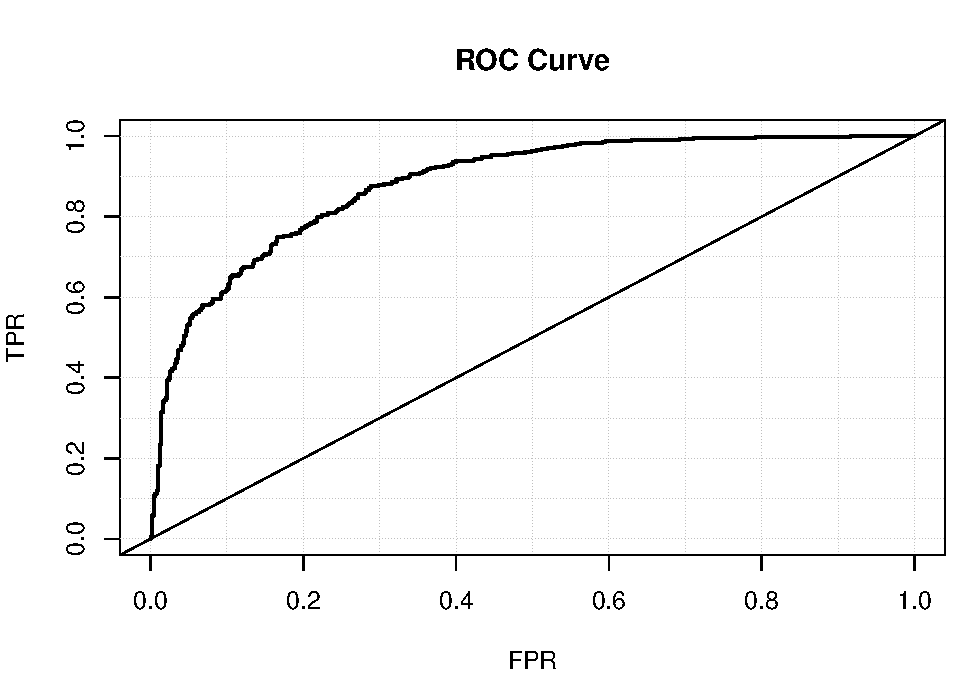
\includegraphics{PTT_Analysis_of_Test_Scores_Unfinished_files/figure-latex/auc-demo-draft-1.pdf}

\begin{Shaded}
\begin{Highlighting}[]
\FunctionTok{print}\NormalTok{(}\StringTok{"done"}\NormalTok{)}
\end{Highlighting}
\end{Shaded}

\begin{verbatim}
## [1] "done"
\end{verbatim}

\begin{Shaded}
\begin{Highlighting}[]
\FunctionTok{print}\NormalTok{(new\_test}\SpecialCharTok{$}\NormalTok{roc.vol)}
\end{Highlighting}
\end{Shaded}

\begin{verbatim}
##      Model     Area      p.value binorm.area
## 1 Model  1 0.881072 5.975725e-97          NA
\end{verbatim}

Or we can retrieve the AUC value directly.

\begin{Shaded}
\begin{Highlighting}[]
\NormalTok{auc\_value }\OtherTok{=}\NormalTok{ new\_test}\SpecialCharTok{$}\NormalTok{roc.vol}\SpecialCharTok{$}\NormalTok{Area}
\FunctionTok{print}\NormalTok{(auc\_value)}
\end{Highlighting}
\end{Shaded}

\begin{verbatim}
## [1] 0.881072
\end{verbatim}

Here is the ROC graph.

More interpretation here

\begin{Shaded}
\begin{Highlighting}[]
\FunctionTok{roc.plot}\NormalTok{(obs\_outcomes,pred,}\AttributeTok{xlab =} \StringTok{"FPR"}\NormalTok{, }\AttributeTok{ylab=}\StringTok{"TPR"}\NormalTok{,}\AttributeTok{show.thres =} \ConstantTok{FALSE}\NormalTok{,}
         \AttributeTok{main=}\FunctionTok{paste}\NormalTok{(}\StringTok{"ROC Curve: AUC ="}\NormalTok{, }\FunctionTok{round}\NormalTok{(auc\_value,}\DecValTok{2}\NormalTok{)))}
\end{Highlighting}
\end{Shaded}

\includegraphics{PTT_Analysis_of_Test_Scores_Unfinished_files/figure-latex/auc-demo-continued-1.pdf}

\hypertarget{more-details}{%
\paragraph{More Details}\label{more-details}}

This ROC graph also shows the probability threshold used for
classification.

More interpretation here

\begin{Shaded}
\begin{Highlighting}[]
\FunctionTok{roc.plot}\NormalTok{(obs\_outcomes,pred,}\AttributeTok{xlab =} \StringTok{"FPR"}\NormalTok{, }\AttributeTok{ylab=}\StringTok{"TPR"}\NormalTok{,}\AttributeTok{show.thres =} \ConstantTok{TRUE}\NormalTok{)}
\end{Highlighting}
\end{Shaded}

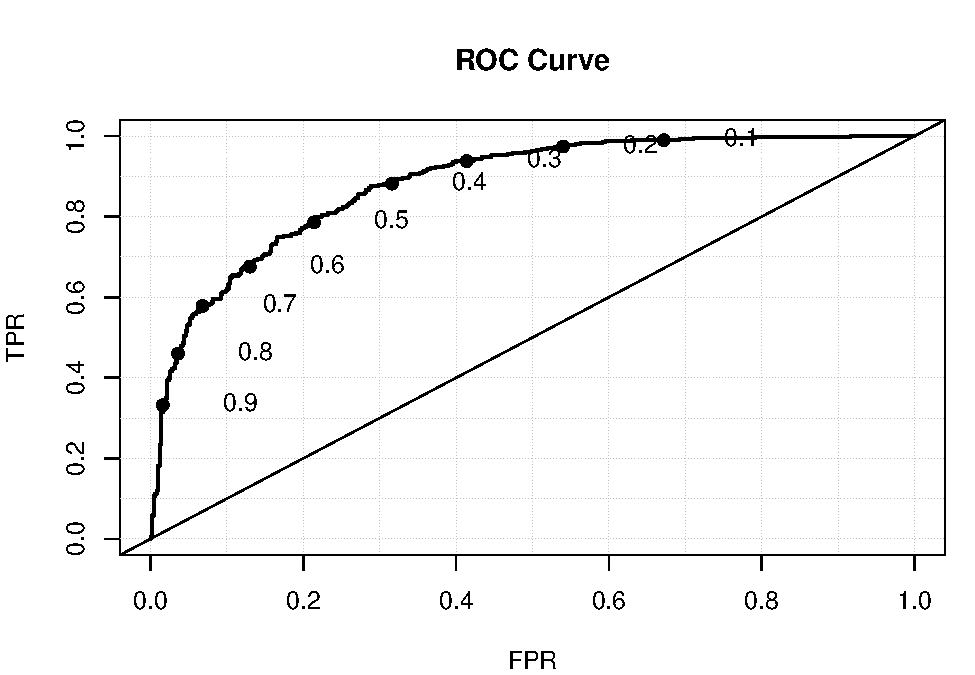
\includegraphics{PTT_Analysis_of_Test_Scores_Unfinished_files/figure-latex/auc-demo-threshold-1.pdf}

What about the underlying data for the ROC graph?

\begin{Shaded}
\begin{Highlighting}[]
\NormalTok{test\_df }\OtherTok{=} \FunctionTok{as.data.frame}\NormalTok{(new\_test}\SpecialCharTok{$}\NormalTok{plot.data)}
\FunctionTok{plot}\NormalTok{(test\_df}\SpecialCharTok{$}\NormalTok{V3, test\_df}\SpecialCharTok{$}\NormalTok{V2, }\AttributeTok{xlab=}\StringTok{"FPR"}\NormalTok{, }\AttributeTok{ylab=}\StringTok{"TPR"}\NormalTok{) }
\end{Highlighting}
\end{Shaded}

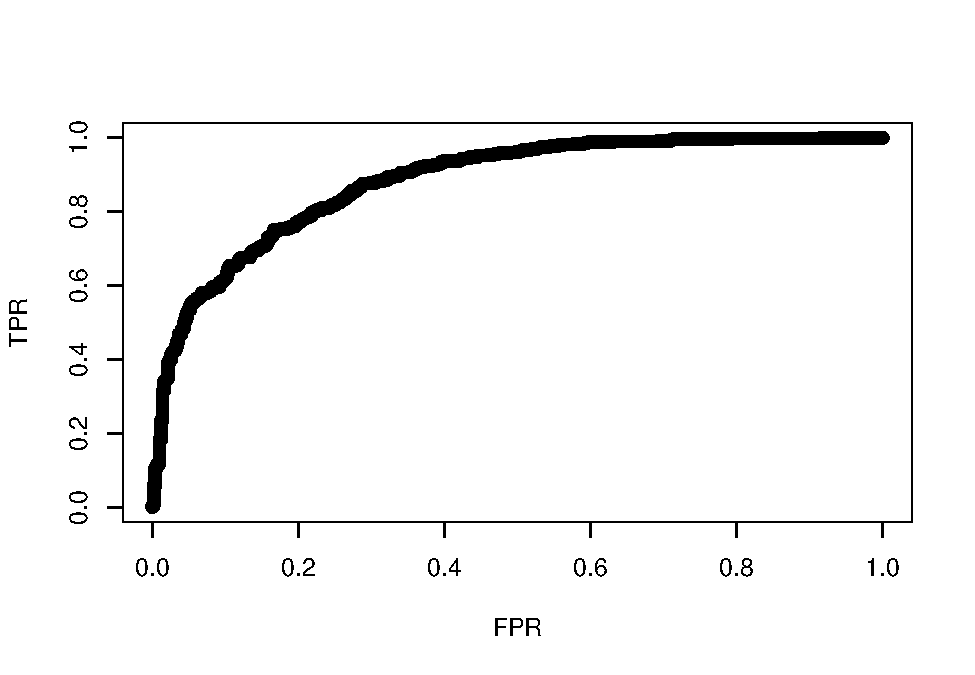
\includegraphics{PTT_Analysis_of_Test_Scores_Unfinished_files/figure-latex/auc-demo-roc-data-1.pdf}

\begin{Shaded}
\begin{Highlighting}[]
\CommentTok{\# test\_df columns:}
\CommentTok{\# V1 = thresholds}
\CommentTok{\# V2 = empirical hit (TPR)}
\CommentTok{\# V3 = false alarm rates (FPR)}
\end{Highlighting}
\end{Shaded}

\hypertarget{roc-prep}{%
\subsubsection{Data Observation and Processing}\label{roc-prep}}

At the beginning of Section \ref{in-sample}, we used 0.5 as the default
probability threshold to classify whether a student would obtain
\textbf{College\_Score} at least 65 or not. That is, the predicted
probability needs to be 0.5 or higher for a datapoint to be predicted as
positive (i.e., getting \textbf{College\_Score} at least 65). This is
acceptable because the data are balanced and 48.9\% of students in the
data made the cut, i.e., obtained \textbf{College\_Score} at least 65.
We are doing this project as an experiment, without trying to optimize
any particular metric. But the probability threshold of 0.5 may not be
appropriate in imbalanced datasets. If a dataset consists of 80\%
samples in the majority category and 20\% samples in the minority
category, the threshold to predict the minority category would be closer
to 80\% to maximize the accuracy.\footnote{\url{https://towardsdatascience.com/tackling-imbalanced-data-with-predicted-probabilities-3293602f0f2}}
Plus, depending on our goal to maximize recall/prediction/other metrics,
we may choose a different threshold for the probability-to-decision
conversion.

In many situations, it is not obvious to determine the probability
threshold to predict a datapoint to be positive. A higher probability
threshold would result in fewer points to be predicted as positive, so
we may not find all of the true positive datapoints. But this model may
be better at classifying true negative datapoints as negative, since the
requirements are high to predict a datapoint to be positive. On the
other hand, a lower probability threshold would predict more points as
positive, increasing the chances of capturing all of the true positive
datapoints. But this may also result in many true negative datapoints
being predicted as positive. Hence there is a tradeoff between recall
and precision when we select the probability threshold.

Let's revisit the leave-one-out cross-validation results from Section
\ref{leave-one-out}, and explore how the probability threshold changes
the accuracy/precision/recall/FPR/FNR. Before deciding on the threshold,
we need to look at the boundary conditions -- the minimum and maximum
predicted probabilities in the data. If the threshold is below the
minimum, the model will predict all points to be true, which is not
useful. If the threshold is above the maximum, the model will predict
all points to be false, which is not useful, either. In the array of
predictive probabilities \texttt{prob\_leave1out}, the minimum is 0.0025
and the maximum is 0.7782. We should choose a probability threshold
between these two values.

\begin{Shaded}
\begin{Highlighting}[]
\NormalTok{check\_prob\_leave1out }\OtherTok{=} \FunctionTok{as.numeric}\NormalTok{(prob\_leave1out)}

\FunctionTok{print}\NormalTok{(}\FunctionTok{paste}\NormalTok{(}\StringTok{"Min prob\_leave1out:"}\NormalTok{, }\FunctionTok{min}\NormalTok{(check\_prob\_leave1out)))}
\end{Highlighting}
\end{Shaded}

\begin{verbatim}
## [1] "Min prob_leave1out: 0.00249702111740674"
\end{verbatim}

\begin{Shaded}
\begin{Highlighting}[]
\FunctionTok{print}\NormalTok{(}\FunctionTok{paste}\NormalTok{(}\StringTok{"Max prob\_leave1out:"}\NormalTok{, }\FunctionTok{max}\NormalTok{(check\_prob\_leave1out)))}
\end{Highlighting}
\end{Shaded}

\begin{verbatim}
## [1] "Max prob_leave1out: 0.778173314094346"
\end{verbatim}

When the probability threshold is set to 0.5 as the default, the
precision is 67\% and the recall is 78\%. We use these numbers as a
comparison baseline. We also show the confusion matrix, so that the
readers can observe the patterns from different probability thresholds.

\begin{Shaded}
\begin{Highlighting}[]
\NormalTok{original\_leave1out }\OtherTok{=}  \FunctionTok{prob\_to\_matrix}\NormalTok{(data\_corr, prob\_leave1out, }\AttributeTok{threshold=}\FloatTok{0.5}\NormalTok{)}
\FunctionTok{print}\NormalTok{(original\_leave1out)}
\end{Highlighting}
\end{Shaded}

\begin{verbatim}
##                 test_pred_65up
## test_actual_65up TRUE FALSE
##            TRUE    72    20
##            FALSE   35    61
\end{verbatim}

\begin{Shaded}
\begin{Highlighting}[]
\NormalTok{original\_results }\OtherTok{=} \FunctionTok{confusion\_to\_measures}\NormalTok{(original\_leave1out)}
\FunctionTok{print}\NormalTok{(}\FunctionTok{round}\NormalTok{(original\_results, }\AttributeTok{digits=}\DecValTok{4}\NormalTok{))}
\end{Highlighting}
\end{Shaded}

\begin{verbatim}
##  Accuracy Precision    Recall       FPR       FNR 
##    0.7074    0.6729    0.7826    0.3646    0.2174
\end{verbatim}

When the probability threshold is 0.7, the precision increased to 82\%,
but the recall decreased to 52\%. A higher probability threshold means
the model is less likely to predict a datapoint to be True, so a
positive prediction is more likely to be actually positive, increasing
the precision. However, the model may miss more datapoints (i.e.,
predict as negative) which are actually positive, resulting in a drop in
the recall.

\begin{Shaded}
\begin{Highlighting}[]
\NormalTok{high\_leave1out }\OtherTok{=} \FunctionTok{prob\_to\_matrix}\NormalTok{(data\_corr, prob\_leave1out, }\AttributeTok{threshold=}\FloatTok{0.7}\NormalTok{)}
\FunctionTok{print}\NormalTok{(high\_leave1out)}
\end{Highlighting}
\end{Shaded}

\begin{verbatim}
##                 test_pred_65up
## test_actual_65up TRUE FALSE
##            TRUE    48    44
##            FALSE   10    86
\end{verbatim}

\begin{Shaded}
\begin{Highlighting}[]
\NormalTok{high\_results }\OtherTok{=} \FunctionTok{confusion\_to\_measures}\NormalTok{(high\_leave1out)}
\FunctionTok{print}\NormalTok{(}\FunctionTok{round}\NormalTok{(high\_results, }\AttributeTok{digits=}\DecValTok{4}\NormalTok{))}
\end{Highlighting}
\end{Shaded}

\begin{verbatim}
##  Accuracy Precision    Recall       FPR       FNR 
##    0.7128    0.8276    0.5217    0.1042    0.4783
\end{verbatim}

When the probability threshold is 0.3, the recall increased from 78\% to
89\%, but the precision decreased from 67\% to 59\%. A lower probability
threshold means the model is more likely to predict a datapoint to be
True, so the model has a better chance of catching most of the
datapoints which are actually positive, increasing the recall. But the
drawback is that when the model predicts a datapoint to be True, the
datapoint has a greater risk of not actually being positive. In other
words, using a low threshold may result in more false positives, hence
reducing the precision.

\begin{Shaded}
\begin{Highlighting}[]
\NormalTok{low\_leave1out }\OtherTok{=} \FunctionTok{prob\_to\_matrix}\NormalTok{(data\_corr, prob\_leave1out, }\AttributeTok{threshold=}\FloatTok{0.3}\NormalTok{)}
\FunctionTok{print}\NormalTok{(low\_leave1out)}
\end{Highlighting}
\end{Shaded}

\begin{verbatim}
##                 test_pred_65up
## test_actual_65up TRUE FALSE
##            TRUE    82    10
##            FALSE   56    40
\end{verbatim}

\begin{Shaded}
\begin{Highlighting}[]
\NormalTok{low\_results }\OtherTok{=} \FunctionTok{confusion\_to\_measures}\NormalTok{(low\_leave1out)}
\FunctionTok{print}\NormalTok{(}\FunctionTok{round}\NormalTok{(low\_results, }\AttributeTok{digits=}\DecValTok{4}\NormalTok{))}
\end{Highlighting}
\end{Shaded}

\begin{verbatim}
##  Accuracy Precision    Recall       FPR       FNR 
##    0.6489    0.5942    0.8913    0.5833    0.1087
\end{verbatim}

\textbf{Remark}: We decided to use the leave-one-out results for ROC-AUC
demonstration, rather than the results from K-fold cross-validation or
separate training and testing datasets. In the outcomes of separate
training and testing datasets (Section \ref{sep-train-test}), only the
testing dataset contains predictive probabilities, and we do not think
the sample size is large enough for the overall evaluation of model
performance. In comparison, both leave-one-out and K-fold
cross-validation (Section \ref{cross-validation}) predict every single
record in the data. The main difference is that in leave-one-out, each
datapoint is predicted by a different training sample. When two
datapoints have the same \textbf{HighSchool$\_$PR} but differ in
\textbf{College$\_$Score}, they will have different predictive
probabilities because the associated training samples are not the same.
On the other hand, K-fold has only \(K\) different subsets, so two
datapoints in the same subset with the same \textbf{HighSchool$\_$PR}
will get the same predicted probability for \textbf{College$\_$Score}.
This can result in many repeated predicted values, which is impractical
in real life.

\hypertarget{roc-auc-results}{%
\subsubsection{Implementation and Results}\label{roc-auc-results}}

\section*{\textcolor{red}{Unfinished below}}

\textcolor{red}{Use the leave-one-out results for ROC-AUC curve, because leave-one-out cross validation predicts every single record in the data.}

Modify from the demo code below

\begin{Shaded}
\begin{Highlighting}[]
\FunctionTok{library}\NormalTok{(verification)}
\FunctionTok{set.seed}\NormalTok{(}\DecValTok{3333}\NormalTok{)}
\NormalTok{obs\_outcomes }\OtherTok{=} \FunctionTok{c}\NormalTok{(}\FunctionTok{rep}\NormalTok{(}\DecValTok{0}\NormalTok{,}\DecValTok{500}\NormalTok{),}\FunctionTok{rep}\NormalTok{(}\DecValTok{1}\NormalTok{,}\DecValTok{500}\NormalTok{))}
\NormalTok{pred\_prob\_1 }\OtherTok{=} \FunctionTok{rnorm}\NormalTok{(}\DecValTok{500}\NormalTok{, }\AttributeTok{mean=}\FloatTok{0.25}\NormalTok{,}\AttributeTok{sd=}\FloatTok{0.3}\NormalTok{)}
\NormalTok{pred\_prob\_2 }\OtherTok{=} \FunctionTok{rnorm}\NormalTok{(}\DecValTok{500}\NormalTok{, }\AttributeTok{mean=}\FloatTok{0.75}\NormalTok{,}\AttributeTok{sd=}\FloatTok{0.3}\NormalTok{)}
\NormalTok{pred }\OtherTok{=} \FunctionTok{c}\NormalTok{(pred\_prob\_1, pred\_prob\_2)}
\NormalTok{new\_test }\OtherTok{=} \FunctionTok{roc.plot}\NormalTok{(obs\_outcomes,pred,}\AttributeTok{xlab =} \StringTok{"FPR"}\NormalTok{, }\AttributeTok{ylab=}\StringTok{"TPR"}\NormalTok{,}\AttributeTok{show.thres =} \ConstantTok{FALSE}\NormalTok{)}

\FunctionTok{print}\NormalTok{(}\StringTok{"done"}\NormalTok{)}
\end{Highlighting}
\end{Shaded}

\begin{verbatim}
## [1] "done"
\end{verbatim}

\begin{Shaded}
\begin{Highlighting}[]
\FunctionTok{print}\NormalTok{(new\_test}\SpecialCharTok{$}\NormalTok{roc.vol}\SpecialCharTok{$}\NormalTok{Area)}
\end{Highlighting}
\end{Shaded}

\begin{verbatim}
## [1] 0.881072
\end{verbatim}

\begin{Shaded}
\begin{Highlighting}[]
\FunctionTok{roc.plot}\NormalTok{(obs\_outcomes,pred,}\AttributeTok{xlab =} \StringTok{"FPR"}\NormalTok{, }\AttributeTok{ylab=}\StringTok{"TPR"}\NormalTok{,}\AttributeTok{show.thres =} \ConstantTok{FALSE}\NormalTok{)}
\end{Highlighting}
\end{Shaded}

\includegraphics{PTT_Analysis_of_Test_Scores_Unfinished_files/figure-latex/auc-another-draft-1.pdf}

\begin{Shaded}
\begin{Highlighting}[]
\CommentTok{\#df = as.data.frame(new\_test$plot.data)}
\CommentTok{\#plot(df$V3,df$V2, xlab="FPR", ylab="TPR") }

\CommentTok{\# df columns:}
\CommentTok{\# V1 = thresholds}
\CommentTok{\# V2 = empirical hit (TPR)}
\CommentTok{\# V3 = false alarm rates (FPR)}
\end{Highlighting}
\end{Shaded}

Draft for ROC-AUC with our data

\begin{Shaded}
\begin{Highlighting}[]
\FunctionTok{library}\NormalTok{(verification)}
\FunctionTok{set.seed}\NormalTok{(}\DecValTok{1234}\NormalTok{)}

\NormalTok{real\_outcomes }\OtherTok{=}\NormalTok{ data\_corr}\SpecialCharTok{$}\NormalTok{College\_Score }\SpecialCharTok{\textgreater{}=}\DecValTok{65}
\NormalTok{pred\_outcomes }\OtherTok{=} \FunctionTok{as.numeric}\NormalTok{(prob\_leave1out)}

\NormalTok{roc\_data\_test }\OtherTok{=} \FunctionTok{roc.plot}\NormalTok{(real\_outcomes, pred\_outcomes, }
                         \AttributeTok{xlab =} \StringTok{"FPR"}\NormalTok{, }\AttributeTok{ylab=}\StringTok{"TPR"}\NormalTok{, }\AttributeTok{show.thres =} \ConstantTok{FALSE}\NormalTok{)}

\FunctionTok{print}\NormalTok{(}\StringTok{"done"}\NormalTok{)}
\end{Highlighting}
\end{Shaded}

\begin{verbatim}
## [1] "done"
\end{verbatim}

\begin{Shaded}
\begin{Highlighting}[]
\FunctionTok{print}\NormalTok{(roc\_data\_test}\SpecialCharTok{$}\NormalTok{roc.vol}\SpecialCharTok{$}\NormalTok{Area)}
\end{Highlighting}
\end{Shaded}

\begin{verbatim}
## [1] 0.7898551
\end{verbatim}

\begin{Shaded}
\begin{Highlighting}[]
\FunctionTok{roc.plot}\NormalTok{(real\_outcomes, pred\_outcomes, }
         \AttributeTok{xlab =} \StringTok{"FPR"}\NormalTok{, }\AttributeTok{ylab=}\StringTok{"TPR"}\NormalTok{,  }\AttributeTok{show.thres =} \ConstantTok{FALSE}\NormalTok{)}
\end{Highlighting}
\end{Shaded}

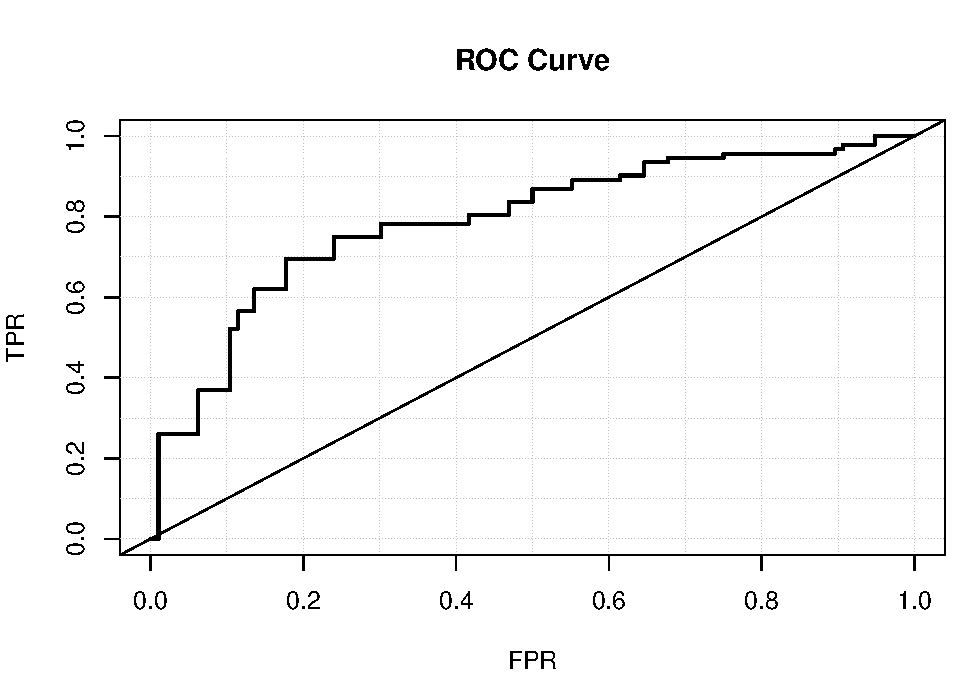
\includegraphics{PTT_Analysis_of_Test_Scores_Unfinished_files/figure-latex/draft-roc-auc-with-data-1.pdf}

\section*{\textcolor{red}{Unfinished above}}

\hypertarget{recap}{%
\section{Recap of the Project}\label{recap}}

This manuscript is a detailed example of a project from data collection
to meaningful insights, and we assume a background equivalent to
Statistics 101. In the end-to-end execution, we also demonstrated good
coding practices such as user-defined functions, descriptive variable
names, and helpful comments in code. These practices in \texttt{R} are
transferable to other programming languages like Python and Java, which
are commonly-used in the tech industry.

We obtained small-scale data that are publicly available and articulated
our thought process in each step. We started with data preprocessing
(i.e., cleaning the data), explored the data, and applied statistical
models to quantify the relationship between the two variables of
interest. The first model we try does not always work out, and the model
validation can reveal more data issues previously undiscovered in the
exploratory phase. Given the new findings, we can try different ways to
continue the analysis.

Our original problem is to find the relationship between high school
entrance exam scores and college entrance exam scores. The exploratory
analysis in Chapter \ref{eda} shows a moderate positive association
between the two sets of scores, with the correlation coefficient 0.50.
However, this does not necessarily mean that the linear regression is
the most appropriate model. Linear regression is widely used, but it is
not a panacea for data analysis. Chapter \ref{linear-reg} states the
four assumptions to be met in linear regression: linearity, nearly
normal residuals, constant variability, and independent observations.
When these assumptions are violated, we should not use the linear
regression model.

Although the linear regression did not work out, we took a deep dive to
understand the data breakdown by high school entrance exam score
category in Chapter \ref{explore-top}. It is possible that a model has
different levels of performance in different ranges of the independent
variable. Exploratory data analysis shows the data are left-skewed,
i.e., much more respondents with high scores than low scores. This
chapter is focused on the top scorers because they account for the
majority of the respondents.

The good news is that we can continue the data analysis through several
ways:

\begin{itemize}
\item
  Transform the data to meet the assumption requirements
\item
  Choose another model to investigate the relationship between the two
  variables
\item
  Reformulate the problem and answer a different question from the data
\end{itemize}

In Chapter \ref{logit-reg}, we reformulated the problem to: Given a
student's high school entrance exam score, estimate the probability of
getting a college entrance exam score of at least 65. This statement
binarizes the outcome of college entrance exam scores, so we discovered
the relationship of the two variables in a different way. Sections
\ref{logit-point-est} and \ref{logit-results} show that when the high
school entrance exam score increases by one percentile, the odds of
``success'' increases by about 16.1\% on average, i.e., getting a
college entrance exam score at least 65. We are 95\% confident that the
odds increase is between 10.6\% and 22.9\%.

After implementing the logistic regression model, we also validated the
results using in-sample prediction (Chapter \ref{validation}) and
out-of-sample prediction (Chapter \ref{out-of-sample}). The accuracy is
approximately 70\% and consistent across both methods of prediction.
About half of the respondents obtained a college entrance exam score at
least 65, so the baseline is around 50\% like a coin-flip. Hence the
logistic regression model is doing much better compared with the
baseline, and the detailed metrics are listed and explained in Section
\ref{cmp-results}.

We also examined the model results by high school entrance exam score
category in Section \ref{another-breakdown}. Since this is a binary
classification model, we focused on the confusion matrices of each
category. For the respondents whose high school entrance exam score in
the 0-79th percentile, the model predicted none of them to obtain a
college entrance exam score of at least 65, but some respondents
actually did succeed. For the respondents in the 80-89th percentile, the
predictions are the same but with a higher proportion of unexpected
successes. The model predictions consist of both success and non-success
outcomes for the respondents in the 90-94th percentile. Finally, the
model predicts all respondents in the 95-99th percentile to obtain a
college entrance exam score of at least 65, and inevitably some of them
did not achieve this. Given the single outcome prediction in most
categories, we added zero columns/rows to ensure the 2x2 size of each
confusion matrix.

\hypertarget{resources}{%
\section{Recommended Resources for Learning}\label{resources}}

We would like to direct readers to resources for learning statistics and
data science, in order to expand their professional skillsets. Online
information is abundant and probably overwhelming, so we decided to
categorize some examples based on difficulty level and the
prerequisites. We also provide a brief description of each resource
including goals and/or applications, so that readers can make informed
decisions in choosing their own professional development activities.
Section \ref{learning-statistics} points to some materials for learning
statistics, while Section \ref{learning-data-science} takes a step
forward to data science and programming.

\hypertarget{learning-statistics}{%
\subsection{Resources for Learning
Statistics}\label{learning-statistics}}

Statistics is the core of data analysis.\footnote{\url{https://datascience.virginia.edu/news/how-much-do-data-scientists-need-know-about-statistics}}
Even with the aid of machine learning algorithms and integrated
computation tools, people still need to know the fundamental concepts in
statistics to appropriately interpret the numbers from the data. For
instance, when you take a sample from the population data, how do you
verify that the sample is a representative sample? How do you interpret
the model coefficients in the output? How do you ensure that all
predictive probabilities are between zero and one? Integrated tools make
it easy to build and run a model, but what's more important is to choose
an appropriate model to implement for the project goal. We also need to
be able to detect and troubleshoot issues in the model output.

Here are some resources we recommend for the path of learning
statistics, from introductory to advanced. Although some readers may be
more interested in data science, learning statistics serves as a
building block to becoming an expert data scientist. Human decisions
also play a key role in getting useful insights from data,\footnote{\url{https://ww2.amstat.org/meetings/sdss/2020/onlineprogram/AbstractDetails.cfm?AbstractID=308230}}
and the statistical skills would help readers in making better decisions
in data.

The Statistics 101 course covers the fundamental statistical concepts
for students to perform data analysis, and the programming component is
often included. For readers who would like a refresher, we recommend the
textbook \emph{OpenIntro Statistics} \citep{diez2019openintro} and the
online course series \emph{Statistics with \texttt{R} Specialization} on
Coursera.\footnote{\url{https://www.coursera.org/specializations/statistics}}
Basic concepts like hypothesis testing and confidence intervals are also
asked in technical interviews for data science jobs. Beware! For an
overview of Bayesian Statistics, we recommend the \emph{Bayesian
Statistics} online course on Coursera,\footnote{\url{https://www.coursera.org/learn/bayesian}}
along with the open-source textbook \emph{An Introduction to Bayesian
Thinking} \citep{clyde2018bayesian101}. At this stage, knowledge of
calculus is helpful but not required.

As the next step beyond the introductory level, we suggest reading
\emph{The Statistical Sleuth: A Course in Methods of Data Analysis}
\citep{ramsey2013statistical}, which is the textbook for
undergraduate-level regression analysis at Duke Statistical
Science.\footnote{\url{https://www2.stat.duke.edu/courses/Fall18/sta210.001/}}
The book covers intermediate topics such as ANOVA (Analysis of Variance)
and multiple linear regression. It also provides data files for case
studies and exercises.\footnote{\url{http://www.statisticalsleuth.com/}}
\emph{Statistics: Unlocking the Power of Data}
\citep{lock2020statistics} is heavily focused on data analysis with real
applications, and this textbook introduces computer simulation methods
like bootstrap intervals and randomization tests for statistical
inference. For a more theoretical overview of mathematical statistics,
we recommend \emph{Probability and Statistics}
\citep{degroot2012probability} where calculus is a prerequisite. A solid
theoretical background helps readers bridge the gap between writing code
and understanding complex statistical models. When the readers go
further in statistics, college-level mathematics becomes increasingly
important. Formulas and equations will gradually appear in the
curriculum, especially calculus for continuous functions and matrix
algebra for discrete datapoints.

For the advanced readers, we recommend the following graduate level
statistics textbooks. Note that multivariate Calculus and matrix algebra
are absolutely necessary at this stage. \emph{A First Course in Bayesian
Statistical Methods} \citep{hoff2009first} explains in detail on how to
perform Bayesian statistical modeling, which is much more comprehensive
than the Bayes' rule (conditional probability). For a focus on linear
models, we suggest \emph{A Modern Approach to Regression with
\texttt{R}} \citep{sheather2009modern} with solid examples, especially
on model validation and residual analysis. \emph{Statistical Inference}
\citep{casella2021statistical} is a must-read if you are interested in
the theory behind statistical concepts such as maximum likelihood
estimation. These textbooks build on statistical concepts that readers
may have already learned at the beginner to intermediate levels. If we
can recommend only one textbook, the one will be \emph{Categorical Data
Analysis} \citep{agresti2003categorical}. This book explains many
generalized linear models in detail, such as logistic regression,
Poisson log-linear model, and proportional hazards for survival analysis
models. There are lots of categorical data in real life, making these
models particularly useful.

There are many other high-quality statistics textbooks in the universe,
and we selected these as a starting point. If the readers are interested
in a data science career, learning statistics builds the foundations and
expands your toolbox to generate insights from data.\footnote{\url{https://towardsdatascience.com/the-difference-between-data-science-and-statistics-168c7062c201}}
We also recommend exploring Kaggle datasets\footnote{\url{https://www.kaggle.com/datasets}}
for hands-on practice. To get closer to analyzing real-world data, we
encourage the readers to attend data hackathons, contribute to
open-source projects, and/or volunteer technical skills at nonprofit
organizations like Statistics Without Borders.\footnote{\url{https://www.statisticswithoutborders.org/}}
These activities are not a comprehensive list, and please feel free to
get creative and carve your own professional path forward.

\hypertarget{learning-data-science}{%
\subsection{Resources for Data Science and
Programming}\label{learning-data-science}}

Since we discussed plenty of statistics resources in the previous
section, we would like to provide a few pointers to \textbf{data
science}, one of the hottest fields in tech. Programming is also
essential to handle data, so we introduce some practical tools that
readers can incorporate them into their data science workflow. (Please
don't get overwhelmed with the massive selection of tools; you can try
one at a time.)

This document is created with \(\mathsf{R}\) Markdown
\citep{r-markdown-pkg},\footnote{\url{https://rmarkdown.rstudio.com/articles_intro.html}}
which has a framework to directly incorporate code and graphs in the
report. This not only reduces the errors from copy-pasting tables and
plots, but also ensures reproducibility of the data analysis
\citep{baumer2014r-markdown}. \(\mathsf{R}\) Markdown can generate
reports in PDF, HTML, or Microsoft Word formats. \(\mathsf{R}\) Markdown
also provides a template for presentation slides, and the output can be
in PDF, HTML, or Microsoft PowerPoint files. Note that PDF output from
\(\mathsf{R}\) Markdown requires the installation of LaTeX.\footnote{\url{https://bookdown.org/yihui/rmarkdown/pdf-document.html}}
(An alternative way is to save the HTML output to a PDF, but this is a
manual step outside the end-to-end pipeline.) For a full book with
multiple chapters, we recommend using the \(\mathsf{R}\) package
\texttt{bookdown} \citep{r-bookdown} for a comprehensive and
reproducible workflow.

The graphs in this manuscript are mainly for demonstration; they are
created using the basic \texttt{plot} function as the default in
RStudio. For advanced data visualization, we highly encourage readers to
use the \(\mathsf{R}\) package \texttt{ggplot2} \citep{ggplot2}. This
package provides much more capability to convey the message in a graph,
and the foundations behind \texttt{ggplot2} are based on \emph{The
Grammar of Graphics} \citep{wilkinson2013grammar}. For a simple and
hands-on guide for data visualization, we recommend the book
\emph{Visualize This} \citep{yau2011visualize} to determine which types
of graphs are most appropriate for which scenarios. On the other hand,
\emph{Semiology of Graphics: Diagrams, Networks, Maps}
\citep{bertin1983semiology} is a comprehensive textbook for data
visualization theory. Concepts such as human perception are
technology-agnostic; the principles apply to almost any tool for data
visualization.

The \(\mathsf{R}\) code is also for demonstration. The author makes
every effort to ensure correctness and readability of the code, but
errors and inconsistencies are inevitable. Since this is an open-source
project on GitHub,\footnote{\url{https://github.com/star1327p/Exam-Scores-PTT}}
readers are welcome to make a pull request and/or report any issues. To
learn more about better coding styles, we recommend the computer science
books \emph{Clean Code} \citep{martin2009clean} and \emph{Code Complete}
\citep{mcconnell2004code}. For complex operations in \(\mathsf{R}\), we
recommend the \(\mathsf{R}\) package \texttt{tidyverse}
\citep{r-tidyverse} because it provides a fast, efficient, and organized
workflow for general data modeling.\footnote{\url{https://www.r-bloggers.com/2018/09/why-learn-the-tidyverse/}}
The book
\textit{$\mathsf{R}$ for Data Science: Import, Tidy, Transform, Visualize, and Model Data}
\citep{wickham2016r} demonstrates an end-to-end cycle of using
\texttt{tidyverse} in data science.

In addition to \(\mathsf{R}\), Python is another commonly-used
programming language in data science. Python is an object-oriented
language which is closer to software development, while \(\mathsf{R}\)
is more focused on statistical models.\footnote{\url{https://www.datacamp.com/tutorial/r-or-python-for-data-analysis}}
Our suggestion is to learn both \(\mathsf{R}\) and Python, so that the
readers get to choose the one that fits their unique needs. (The author
does not have a strong personal preference, so she often chooses the one
that her collaborators use to better leverage their existing code.)
After you know a programming language, it would not be difficult to
learn a new one because many concepts are similar, such as \texttt{for}
loops and user-defined functions. Don't worry!

\hypertarget{personal-remarks}{%
\section{Final: Personal Scores and Remarks}\label{personal-remarks}}

This manuscript is created because the author reflected on her own
experience regarding high school and college entrance exams. Instead of
dwelling on the past, the author decided to redirect her energy to
something more meaningful and constructive. She leveraged the
opportunity to apply her data science and research skills. In addition
to statistical analysis, she also wanted to demonstrate full
reproducibility of the project. Inspired by
\citet{baumer2014r-markdown}, the author decided to incorporate
\(\mathsf{R}\) Markdown as a reproducible analysis tool into
introductory statistics. She also designed her own template to create
LaTeX Beamer PDF slides from \(\mathsf{R}\) Markdown,\footnote{\url{https://github.com/star1327p/r-beamer-template}}
in which she included some commonly-used LaTeX functions.

The author scored \textbf{HighSchool\_PR} 95 in Year 2004, but she got
admitted to Taipei First Girls' High School because the special class
for math and science track had a separate admission process at that
time. Taipei First Girls' High School\footnote{\url{http://web.fg.tp.edu.tw/~tfghweb/EnglishPage/index.php}}
usually requires \textbf{HighSchool\_PR} 99 for admission, with few
exceptions such as recruited athletes\footnote{\url{https://www.sa.gov.tw/PageContent?n=1265}}
and students with disabilities.\footnote{\url{http://www.rootlaw.com.tw/LawArticle.aspx?LawID=A040080080001900-1020822}}
Several years later, the policy changed so that students had to be
admitted to the high school first in order to try for the special class
placement within. Most students in the special class had
\textbf{HighSchool\_PR} 99 anyway, and the author was one of the few who
did not. Hence the author wondered whether she would have similar
academic performance, had she enrolled in a different high school
commensurate to \textbf{HighSchool\_PR} 95 in Taipei, Taiwan.

The author got \textbf{College\_Score} 69 on the General Scholastic
Ability Test (GSAT) in Year 2007. She applied to several colleges, and
one of them offered her early admission.\footnote{\url{https://sites.google.com/site/christinepeijinnchai/resume-cv}}
However, she was not satisfied with the outcome, so she decided to try
for the Advanced Subjects Test (AST). She obtained an excellent score on
the AST and got admitted to The Department of Electrical Engineering at
National Taiwan University (NTUEE), one of the top colleges in Taiwan.
NTUEE\footnote{\url{https://web.ee.ntu.edu.tw/eng/index.php}} typically
requires full marks (15 out of 15) in English, mathematics, and science
in \textbf{College\_Score} for the early admission through
GSAT.\footnote{\url{https://university.1111.com.tw/univ_depinfo9.aspx?sno=100102\&mno=520101}}
Most students at NTUEE had a \textbf{College\_Score} of 70 or higher, at
the time when 75 was the max possible score. But still a significant
number of students got admitted through the AST in July, regardless of
their GSAT score.

\hypertarget{comparison-with-the-data}{%
\subsection{Comparison with the Data}\label{comparison-with-the-data}}

The author's high school and college entrance exam scores are indicated
as the red dot in the scatterplot below from Section \ref{bivariate}. We
also added the reference lines for \textbf{HighSchool\_PR} 80 and
\textbf{College\_Score 60}. \textbf{HighSchool\_PR} 95 and
\textbf{College\_Score} 69 are definitely above-average scores, despite
imperfect.

\begin{Shaded}
\begin{Highlighting}[]
\FunctionTok{plot}\NormalTok{(data\_corr}\SpecialCharTok{$}\NormalTok{HighSchool\_PR, data\_corr}\SpecialCharTok{$}\NormalTok{College\_Score,}
     \AttributeTok{main =} \StringTok{"High School and College Entrance Exam Scores"}\NormalTok{,}
     \AttributeTok{xlab=}\StringTok{"HighSchool\_PR"}\NormalTok{,}
     \AttributeTok{ylab=}\StringTok{"College\_Score"}\NormalTok{)}

\FunctionTok{abline}\NormalTok{(}\AttributeTok{h=}\DecValTok{60}\NormalTok{,}\AttributeTok{v=}\DecValTok{80}\NormalTok{)}
\FunctionTok{points}\NormalTok{(}\AttributeTok{x=}\DecValTok{95}\NormalTok{, }\AttributeTok{y=}\DecValTok{69}\NormalTok{, }\AttributeTok{col=}\StringTok{"red"}\NormalTok{, }\AttributeTok{pch=}\DecValTok{19}\NormalTok{)}
\end{Highlighting}
\end{Shaded}

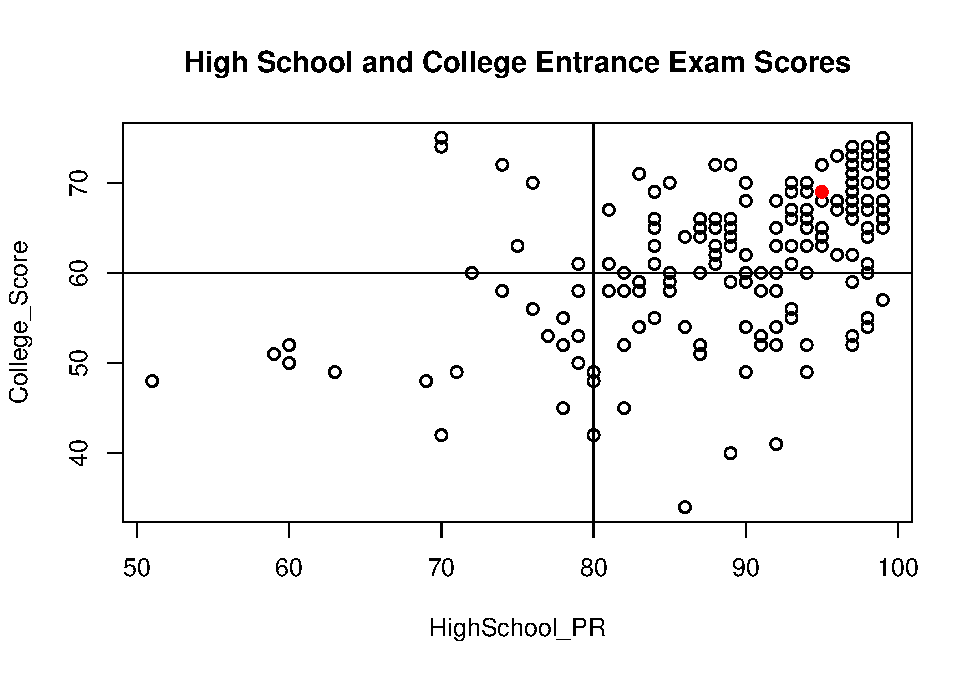
\includegraphics{PTT_Analysis_of_Test_Scores_Unfinished_files/figure-latex/bivariate-dup-1.pdf}

Let's examine all of the \textbf{College\_Score} datapoints given
\textbf{HighSchool\_PR} 95. There are seven points in the data, with
median 68 and mean about 67.6. One of them is \textbf{College\_Score}
69, the same score as the author's. (She personally did not respond to
this survey in 2015 because she discovered this announcement a few years
later.)

\begin{Shaded}
\begin{Highlighting}[]
\FunctionTok{sort}\NormalTok{(data\_corr}\SpecialCharTok{$}\NormalTok{College\_Score[}\FunctionTok{which}\NormalTok{(data\_corr}\SpecialCharTok{$}\NormalTok{HighSchool\_PR }\SpecialCharTok{==} \DecValTok{95}\NormalTok{)])}
\end{Highlighting}
\end{Shaded}

\begin{verbatim}
## [1] 63 64 65 68 69 72 72
\end{verbatim}

Let's also inspect the nearby values, i.e., the \textbf{College\_Score}
values given \textbf{HighSchool\_PR} 94 or 96.

For \textbf{HighSchool\_PR} 94, there are ten \textbf{College\_Score}
values in the data. The median is 66, and the mean is 63. The author's
\textbf{College\_Score} would be the second highest score in this batch.

\begin{Shaded}
\begin{Highlighting}[]
\FunctionTok{sort}\NormalTok{(data\_corr}\SpecialCharTok{$}\NormalTok{College\_Score[}\FunctionTok{which}\NormalTok{(data\_corr}\SpecialCharTok{$}\NormalTok{HighSchool\_PR }\SpecialCharTok{==} \DecValTok{94}\NormalTok{)])}
\end{Highlighting}
\end{Shaded}

\begin{verbatim}
##  [1] 49 52 60 63 65 66 66 66 67 69 70
\end{verbatim}

For \textbf{HighSchool\_PR} 96, there are five \textbf{College\_Score}
values in the data. The median is 67, and the mean is 67.4. The author's
\textbf{College\_Score} would still be the second highest in this batch.

\begin{Shaded}
\begin{Highlighting}[]
\FunctionTok{sort}\NormalTok{(data\_corr}\SpecialCharTok{$}\NormalTok{College\_Score[}\FunctionTok{which}\NormalTok{(data\_corr}\SpecialCharTok{$}\NormalTok{HighSchool\_PR }\SpecialCharTok{==} \DecValTok{96}\NormalTok{)])}
\end{Highlighting}
\end{Shaded}

\begin{verbatim}
## [1] 62 67 67 68 73
\end{verbatim}

Finally, let's explore the \textbf{College\_Score} values of
\textbf{HighSchool\_PR} 97-99. There are 58 datapoints, which account
for 30.8\% of the total data. The median of \textbf{College\_Score} is
70, and the mean is 68. Note that the max possible
\textbf{College\_Score} is 75, and few respondents achieved 74 or 75 in
the entire dataset. In the earlier graph of this subsection,
\textbf{College\_Score} 69 is about in the middle of the
\textbf{College\_Score} datapoints for \textbf{HighSchool\_PR} 97-99.
This observation is similar to what we discovered in the subset.

\begin{Shaded}
\begin{Highlighting}[]
\NormalTok{pr97to99 }\OtherTok{=} \FunctionTok{sort}\NormalTok{(data\_corr}\SpecialCharTok{$}\NormalTok{College\_Score[}\FunctionTok{which}\NormalTok{(data\_corr}\SpecialCharTok{$}\NormalTok{HighSchool\_PR }\SpecialCharTok{\%in\%} \FunctionTok{c}\NormalTok{(}\DecValTok{97}\NormalTok{,}\DecValTok{98}\NormalTok{,}\DecValTok{99}\NormalTok{))])}

\FunctionTok{print}\NormalTok{(pr97to99)}
\end{Highlighting}
\end{Shaded}

\begin{verbatim}
##  [1] 52 53 54 55 57 59 60 61 62 64 65 65 65 66 66 66 67 67 67 67 68 68 68 68 68
## [26] 69 69 70 70 70 70 70 71 71 71 71 71 71 71 71 72 72 72 72 72 72 72 73 73 73
## [51] 73 73 73 73 74 74 74 75
\end{verbatim}

\begin{Shaded}
\begin{Highlighting}[]
\FunctionTok{print}\NormalTok{(}\FunctionTok{paste}\NormalTok{(}\StringTok{"Number of datapoints:"}\NormalTok{,}\FunctionTok{length}\NormalTok{(pr97to99)))}
\end{Highlighting}
\end{Shaded}

\begin{verbatim}
## [1] "Number of datapoints: 58"
\end{verbatim}

\begin{Shaded}
\begin{Highlighting}[]
\FunctionTok{print}\NormalTok{(}\FunctionTok{paste}\NormalTok{(}\StringTok{"Median College\_Score:"}\NormalTok{,}\FunctionTok{median}\NormalTok{(pr97to99)))}
\end{Highlighting}
\end{Shaded}

\begin{verbatim}
## [1] "Median College_Score: 70"
\end{verbatim}

\begin{Shaded}
\begin{Highlighting}[]
\FunctionTok{print}\NormalTok{(}\FunctionTok{paste}\NormalTok{(}\StringTok{"Mean College\_Score:"}\NormalTok{,}\FunctionTok{round}\NormalTok{(}\FunctionTok{mean}\NormalTok{(pr97to99), }\AttributeTok{digits=}\DecValTok{1}\NormalTok{)))}
\end{Highlighting}
\end{Shaded}

\begin{verbatim}
## [1] "Mean College_Score: 68"
\end{verbatim}

Given the author's \textbf{HighSchool\_PR} 95 score,
\textbf{College\_Score} 69 is an above-average outcome. Although it is
somewhat unfair to compare \textbf{HighSchool\_PR} 95 with
\textbf{HighSchool\_PR} 97 as a nearby value, \textbf{College\_Score} 69
is only one point below the median \textbf{College\_Score} of the
\textbf{HighSchool\_PR} 97-99 group. We do not know whether the positive
outcome is due to the fact that the author studied extra hard given the
more competitive environment in her high school, and/or she received
more resources than most respondents with \textbf{HighSchool\_PR} 95.

The most prestigious high schools in Taipei typically requires
\textbf{HighSchool\_PR} 97 or higher.\footnote{\url{https://cclccl-life.blogspot.com/2013/06/blog-post_9.html}}
Students in Taipei with \textbf{HighSchool\_PR} 97 may receive
significantly more resources than the ones with \textbf{HighSchool\_PR}
95, despite the difference is only two percentage points. This
phenomenon is less likely in areas where the \textbf{HighSchool\_PR}
requirement is not as high in their top local high schools.

\hypertarget{comparison-with-the-model-prediction}{%
\subsection{Comparison with the Model
Prediction}\label{comparison-with-the-model-prediction}}

We also apply the logistic regression model in Section
\ref{threshold-65}, which predicts the probability of a respondent
achieving \textbf{College\_Score} at least 65 with his/her
\textbf{HighSchool\_PR}. Given the author's \textbf{HighSchool\_PR} 95
score, the predictive probability is about 64.6\% in terms of how likely
she would have achieved \textbf{College\_Score} at least 65. As a
reference, Section \ref{logit-point-est} shows that given
\textbf{HighSchool\_PR} 99, the estimated probability to achieve this is
76.9\%. The numbers made the author feel better, because she still had a
good chance of getting \textbf{College\_Score} at least 65 given her
original \textbf{HighSchool\_PR}.

\begin{Shaded}
\begin{Highlighting}[]
\NormalTok{original\_model }\OtherTok{=} \FunctionTok{glm}\NormalTok{(CS\_65up }\SpecialCharTok{\textasciitilde{}}\NormalTok{ HighSchool\_PR, }\AttributeTok{data=}\NormalTok{data\_corr, }\AttributeTok{family=}\StringTok{"binomial"}\NormalTok{)}
\CommentTok{\# summary(original\_model)}

\NormalTok{my\_data }\OtherTok{=} \FunctionTok{data.frame}\NormalTok{(}\AttributeTok{HighSchool\_PR =} \DecValTok{95}\NormalTok{, }\AttributeTok{College\_Score =} \DecValTok{69}\NormalTok{, }\AttributeTok{CS\_65up =} \ConstantTok{TRUE}\NormalTok{)}

\NormalTok{pred\_prob }\OtherTok{=} \FunctionTok{predict.glm}\NormalTok{(original\_model, my\_data, }\AttributeTok{type=}\StringTok{"response"}\NormalTok{)}
\CommentTok{\# type="response" gives the predicted probabilities}

\NormalTok{pred\_prob}
\end{Highlighting}
\end{Shaded}

\begin{verbatim}
##         1 
## 0.6464676
\end{verbatim}

Again, the logistic regression model assumes all else are held equal. We
also assume that most respondents attended a high school whose admission
requirement is about their own \textbf{HighSchool\_PR}. From this data,
we cannot measure the effect from impostor syndrome -- one decided to
study extra hard to compensate that he/she had a much lower
\textbf{HighSchool\_PR} compared with his/her classmates in high school.
Given the goal of demonstrating statistical methods in this project, we
do not think it is practical to find such people and compare their
scores with the people who did not receive this opportunity. This can be
a full research project in the education field.

\hypertarget{acknowledgments}{%
\section*{Acknowledgments}\label{acknowledgments}}
\addcontentsline{toc}{section}{Acknowledgments}

The author would like to thank Dr.~Mine Cetinkaya-Rundel and Dr.~David
Banks at Duke University; they both motivated the author to teach
statistics and create reproducible work in \(\mathsf{R}\). The author is
also grateful to her Microsoft colleagues Smit Patel and Dylan Stout for
troubleshooting GitHub issues.

The author would also like to acknowledge Dr.~Cliburn Chan and
Dr.~Janice McCarthy for introducing her to GitHub in the statistical
computation course at Duke University. This provided her the foundations
to use GitHub as a modern version control system in the first place.

Finally, the author gives a special mention to her significant other,
Hugh Hendrickson, for all his support in the author's professional
career development.

\renewcommand\refname{References}
  \bibliography{references.bib}

\end{document}
